% !TEX program = lualatex
% ======================================================================
\documentclass[12pt,a4paper,twoside,openright]{book}

%───────── Auxiliary packages ──────────────────────────────────────────
\usepackage{blindtext}
\usepackage{mwe}
\usepackage{csquotes}
\usepackage{graphicx}
\usepackage{float}
\usepackage{subcaption}
\usepackage{booktabs}
\usepackage{xltabular}
\usepackage{siunitx}
\usepackage{amsmath,amssymb}
\usepackage{algorithm}
\usepackage{algpseudocode}
\usepackage{listings}
\usepackage{xurl}
\usepackage{nomencl}
\makenomenclature
\usepackage[
  backend=biber,
  style=numeric,
  sorting=nyt
]{biblatex}
\addbibresource{references.bib}

% Listings config
\lstset{
  basicstyle=\ttfamily\small,
  numbers=left,
  numberstyle=\tiny,
  columns=fullflexible,
  frame=single,
  breaklines=true,
  tabsize=2
}

%───────── Template, covers, back cover ────────────────────────────────
\usepackage{template/sty_files/template-TFGspanish-uma}

\usepackage{template/sty_files/cotutor_cover-blueuma}
\usepackage{template/sty_files/cotutor_cover-whiteuma}

\usepackage{template/sty_files/backcover-uma}

\renewcommand{\lstlistingname}{Listado}

%======================================================================
\begin{document}

% Evita que LaTeX estire verticalmente las páginas cortas (lo que despegaba los
% títulos de su texto). El espacio sobrante queda al pie en lugar de repartido.
\raggedbottom

%────────────────────── Blue front cover (Cotutor) ───────────────────────

\MakeBlueUMACover{
  degree     = {Grado en Ingeniería Informática},
  mencion    = {Mención en Sistemas de la información},
  titleES    = {Diseño de un sistema de telemetría para el análisis, visualización y ayuda a la toma de decisiones 
aplicado al deporte de motor y alta competición},
  titleEN    = {Design of a telemetry system for analysis, visualization and decision support applied to 
high-performance motorsport },
  author     = {Darío Alessandro Di Totaro Ruíz},
  tutor      = {Francisco Javier Ferrer Urbano },
  dept       = {Departamento de Lenguajes y Ciencias de la Computación},
  cityDate   = {Málaga, Mayo, 2026},
  logoLeft   = {template/logos/NEG-uma-logo.png},
  logoRight  = {template/logos/NEG-etsi-logo.png}
}

\frontmatter

%────────────────────── Abstracts ──────────────────────────────────────
\renewcommand{\abstractname}{Resumen}
\begin{abstract}
Este trabajo centra sus esfuerzos en el desarrollo de una herramienta gratuita de código abierto
que permita a los usuarios analizar los múltiples aspectos fundamentales que influyen en el deporte de motor.
Dada la amplitud de las diferentes categorías dentro de esta disciplina nos centraremos en la categoría más influyente, la Fórmula 1.
Mediante un \emph{dashboard}, el usuario obtiene una visualización detallada de los pilotos y escuderías presentes en el transcurso de un gran premio, 
facilitando un análisis sencillo de cada carrera.

El principal objetivo de este proyecto es proporcionar una herramienta intuitiva para personas con un conocimiento de base del deporte, 
personas con un interés por el \emph{simracing} o usuarios que quieran introducirse en la modalidad de una forma más técnica.
Los usuarios pueden interactuar con los diferentes apartados y analizar detalles que puedan ayudar a mejorar su conocimiento sobre el deporte o comportamiento de los monoplazas analizando
resultados, ritmo de carrera, distintas estrategias, fuerzas G del trazado o estrés del neumático.
El desarrollo se ha llevado a cabo utilizando Streamlit, un \emph{framework} de Python de código abierto que permite construir aplicaciones web para el análisis de datos con capacidad para integrar
gráficos. Python se ha utilizado como lenguaje aprovechando bibliotecas como NumPy, Pandas o Plotly para los distintos procesos que conlleva el manejo de datos.
Se obtienen datos del monoplaza mediante el uso de APIs públicas como Ergast y la biblioteca FastF1 para la recolección de datos de la API de la Fórmula 1 así
como una caché local para mejorar los tiempos de carga.

\noindent 
Se ha identificado como área de posible expansión la integración de datos de otras competiciones con mayor accesibilidad de datos, como el WEC (\emph{World Endurance Championship}) o categorías de Fórmula inferiores.
El resultado es una herramienta de análisis post-sesión que integra en una interfaz la visualización de telemetría, estrategia de carrera y clasificación automática de estilos de pilotaje.

\noindent\textbf{Palabras clave:} Fórmula 1, Análisis de datos, Python,
Telemetría, Streamlit, Dashboard, Deportes
\end{abstract}

\renewcommand{\abstractname}{Abstract}
\begin{abstract}
This work centers its efforts on the development of a free open-source tool that allows users to analyze the multiple fundamental aspects that influence motorsport.
Given the breadth of the different categories within this discipline, we will focus on the most influential category, Formula 1.
Through a dashboard the user obtains a detailed visualization of the drivers and teams present during the course of a grand prix, facilitating a simple analysis of each race.

The main objective of this project is to provide an intuitive tool for people with a base knowledge of the sport, people with an interest in simracing or users who want to introduce themselves to the modality in a more technical way.
Users can interact with the different sections and analyze details that can help to improve their knowledge about the sport or behavior of the single-seaters analyzing results, race pace, different strategies, G-forces of the track or tire stress.
The development has been carried out based on Streamlit, an open-source Python framework that allows building web applications for data analysis with the capacity to integrate graphics. Python has been used as the language taking advantage of libraries like NumPy, Pandas or Plotly for the different processes that data handling entails.
Data of the car is obtained through the use of public APIs like Ergast and the FastF1 library for data collection from the Formula 1 API as well as a local cache to improve loading times.

\noindent
It has been identified as an area of possible expansion the integration of data from other competitions with greater data accessibility, such as the WEC (World Endurance Championship) or lower Formula categories.
The result is a post-session analysis tool that integrates telemetry visualization, race strategy and automatic classification of driving styles into a single interface, bringing to the average fan an analysis previously reserved for the teams.

\noindent\textbf{Keywords:} Formula 1, Data analysis, Python, Telemetry, Streamlit, Dashboard, Sports
\end{abstract}

%──────────────── Acknowledgments ───────────────────────────────────────
\begin{umaacknowledgments}
A mi familia, lo primero y lo más importante. Por estar siempre, por el apoyo incondicional en cada paso de estos años y por no dejarme tirar la toalla cuando tocaba. Nada de esto habría sido posible sin vosotros, y este trabajo es tan vuestro como mío.

A mis amigos y compañeros de carrera, por las horas en la biblioteca y las que no fueron en la biblioteca, por hacer que estos años hayan merecido la pena.

A mi tutor, Francisco Javier Ferrer Urbano, por su orientación y seguimiento constante a lo largo del desarrollo de este trabajo.

Y, en general, a todos los que de una forma u otra han caminado conmigo hasta aquí. Gracias.
\end{umaacknowledgments}

%────────────────────── TOC and lists ──────────────────────────────────
\clearpage
\tableofcontents
\clearpage
\listoffigures
\clearpage
\listoftables
%────────────────────── Índice de Listados ─────────────────────────────
\makeatletter
\cleardoublepage
\phantomsection
\chapter*{Índice de Listados}
\addcontentsline{toc}{chapter}{Índice de Listados}
\markboth{Índice de Listados}{Índice de Listados}
\vspace{10pt}
\@starttoc{lol}
\makeatother
\clearpage



\mainmatter
%────────────────────── Capítulo 1 - Introducción ───────────────────────
\chapter{Introducción y Objetivos}
\section{Introducción}
La Fórmula 1 es la categoría con más prestigio del automovilismo deportivo y uno de los entornos tecnológicos más exigentes de todo el mundo.
Cada coche incorpora cerca de 300 sensores que generan 2 GB de datos por vuelta de forma aproximada. Estos datos abarcan desde la temperatura individual de cada neumático
hasta la presión del aire y la carga aerodinámica sobre puntos concretos de la carrocería. Esta vasta cantidad de información construye la base sobre la que los equipos terminarán tomando decisiones estratégicas en tiempo real:
cuándo realizar una parada en boxes, cómo ajustar el balance de carga en el monoplaza o cómo adaptar el estilo de conducción según el estado de la pista y del propio vehículo.
Estos datos no solo influyen para las carreras en sí sino a lo largo de toda la temporada para poder desarrollar el coche aplicando mejoras a las piezas de la carrocería.

\noindent La relación entre la Fórmula 1 y los datos no es reciente. Ya en la década de 1980, equipos como McLaren comenzaron a introducir sistemas rudimentarios de telemetría transmitiendo parámetros básicos del motor al garaje. Con la llegada de los sistemas de adquisición de datos digitales la información es mucho más accesible multiplicando los datos disponibles
convirtiendo a la figura del ingeniero en una figura con casi tanta importancia como la del propio piloto. Hoy, un fin de semana genera varios terabytes de información que es analizada en tiempo real desde los \textit{command centers} de las fábricas en Milton Keynes, Maranello o Brackley, a miles de kilómetros del circuito.
La telemetría dejó de ser una herramienta de diagnóstico para convertirse en el pilar central de la toma de decisiones en la categoría más exigente del automovilismo.

\medskip \noindent Sin embargo la mayor parte de esta información es altamente confidencial ya que las escuderías la consideran como secretos empresariales e información competitiva.
Los datos que se publican de forma oficial son un subconjunto altamente reducido como los tiempos de vuelta, compuestos del neumático, posición GPS y telemetría básica del piloto. La librería de código abierto FastF1 permite acceder a estos datos históricos de una forma estructurada y ha impulsado
en los últimos años una comunidad creciente de análisis aficionado.

\noindent A pesar de la disponibilidad de estos datos, las herramientas existentes para su explotación presentan limitaciones importantes: Son fragmentarias, cada \textit{script} analiza un solo aspecto de forma aislada, requieren conocimientos de programación para su uso y no ofrecen
una experiencia integrada que permita navegar entre los distintos tipos de análisis sobre una misma sesión. Por otro lado las opciones propietarias, que son las que las propias escuderías utilizan, tienen un elevado coste de licencia por lo que no es una opción recomendada para el aficionado promedio.
Los usuarios carecen de una plataforma unificada y gratuita que les permita explorar el máximo de telemetría posible con profundidad e interactividad que los datos permiten.

\noindent \textit{Telemetry Analysis and Lap Optimization System} (TALOS de ahora en adelante) nace para cubrir este hueco. Se trata de un sistema de soporte a la decisión (DSS) orientado al análisis interactivo de telemetría histórica de Fórmula 1, construido sobre datos públicos y herramientas de código abierto.
Es decir, TALOS opera sobre datos ya registrados realizando un análisis \textbf{post-sesión} o asíncrono, una vez ha concluido la sesión. No se trata por tanto de un sistema de telemetría a tiempo real como los que emplean los equipos durante la competición, sino de una herramienta de estudio y exploración a posteriori.
\section{Motivación}
El interés técnico de este trabajo reside en el conjunto de varias disciplinas de la Ingeniería informática aplicadas a un dominio de datos real. La telemetría obtenida no es un conjunto de datos completamente limpio:
presenta muestreo irregular, valores ausentes y muestras irregulares además que muestra una frecuencia mucho más baja de datos que los sensores que usan las escuderías.
Procesarla correctamente exige técnicas de filtrado, en particular el filtro de Savitzky-Golay~\cite{savgol1964} para preservar derivadas mientras se elimina el ruido de alta frecuencia.

\noindent Sobre esta base se construyen 2 motores de inferencia. El primero es un clasificador de circuitos basado en reglas sobre características extraidas de un conjunto extenso de vueltas, esto categoriza el trazado en una de cinco tipologías.
El segundo es un clasificador de estilos de conducción sobre métricas de comportamiento de piloto. Ambos clasificadores están basados en \textit{K-Means} no supervisado.

\noindent Desde el punto de vista funcional, la motivación principal es hacer accesible un tipo de análisis reservado a ingenieros de escudería y ponerlo al alcance del aficionado. Sirve como punto de entrada
al aficionado promedio que desee entender cómo funciona el deporte con una mayor profundidad e incluso puede atraer a gente nueva al deporte, explicando cómo funciona todo de una manera detallada y que una persona con poco conocimiento sobre el dominio del deporte pueda entender.
TALOS no compite con las herramientas profesionales, sino que traslada su filosofía analítica vista desde un punto gratuito e interactivo.

\noindent El origen personal de este trabajo es anterior a la ingeniería. La Fórmula 1 fue durante años un ritual familiar de los domingos habiendo incluso estado en circuitos de forma presencial. Este interés se retomó en la etapa universitaria con una nueva dimensión, la del \textit{simracing}, donde mejorar los tiempos de vuelta exige
exactamente el mismo tipo de análisis que realizan los ingenieros de pista aunque con datos mucho más limitados.
Fue esa mentalidad de optimización y entender el dato la que orientó la elección del tema. La propuesta inicial era más ambiciosa, un sistema de predicción de estrategia de carreras. Sin embargo durante las fases tempranas quedó patente que la validación de dichas predicciones era inviable sin acceso a la información que las escuderías no publican.
El proyecto pivotó hacia un objetivo más sólido y validable: construir una herramienta de análisis e interpretación de la telemetría existente, que es precisamente lo que TALOS es.

\section{Objetivos}
La Fórmula 1 es hoy en día un deporte difícil de entender por primera vez. No porque sea aburrido, sino porque ocurren demasiadas cosas a la vez: estrategias de neumáticos en vueltas tempranas, adelantamientos que se "cocinan" con más de tres vueltas de antelación, diferencias
de rendimiento entre pilotos del mismo equipo. El aficionado nuevo se encuentra con un deporte que no solo exige ver las carreras, sino que exige contexto antes de poder disfrutarlo, y ese contexto no está siempre disponible de forma accesible.

\noindent Este trabajo nace con la intención de ser este contexto. No un sustituto de la carrera sino una herramienta que permita entenderla mejor, antes o después de verla. Que un usuario pueda abrir la aplicación tras el gran premio y entender visualmente y analíticamente por qué un piloto fue el más veloz en un sector, o qué diferencia
hay entre el punto de frenada con otro piloto, como acabó la carrera, clasificación o entrenamientos. Alguien que lleva siguiendo el deporte desde hace años pueda encontrar en los datos alguna confirmación o una contradicción de lo que creía saber.

\noindent Hay también un público al que no se suele mencionar por pertenecer a un nicho de espectadores que hoy en día se está volviendo más grande y representa quizás el caso de uso más interesante: el jugador de \textit{simracing}. Quien practica simulación de carreras ya tiene una intuición sobre lo que significa
perder tiempo en una curva o gestionar los neumáticos, pero rara vez tiene acceso a datos reales con los que calibrar esa intuición. Esta herramienta puede ser para ese usuario lo que un ingeniero de datos sería en un equipo profesional. Nótese que la herramienta está diseñada de forma modular, por lo que es posible añadir una nueva funcionalidad para ver los 
propios datos de telemetría capturando paquetes UDP de videojuegos de Fórmula 1 o simuladores como Assetto Corsa.

\noindent Existe además un tercer perfil al que pocas herramientas prestan atención: el que llega al deporte sin bagaje previo. Alguien que empieza a ver carreras y no entiende por qué un coche que va primero puede acabar tercero, o qué significa que un piloto \textit{gestione} los neumáticos.
Para ese perfil la herramienta puede funcionar como punto de entrada: no como un tutorial sino como un espejo en el que ver reflejado lo que ha ocurrido con datos reales detrás. Ver la telemetría no requiere saber de ingeniería, requiere de curiosidad, y eso es algo que la herramienta no puede ni necesita exigir.
\noindent En ese sentido, el proyecto no tiene un tipo único de usuario sino un espectro. En un extremo, el aficionado ocasional que quiere entender por qué su piloto favorito perdió la carrera, en el otro, el entusiasta técnico que quiere comparar las fuerzas G de dos trazadas distintas. TALOS está diseñado para ser útil en ambos extremos sin resultar intimidante en ninguno de los dos.

\noindent Lo que une todos estos casos de uso es la misma convicción: que los datos de la Fórmula 1 ya son públicos y accesibles, y que lo que faltaba no era más información sino una forma mejor de explorarla. Ese es el hueco que este trabajo intenta cubrir.

\noindent En síntesis, los objetivos específicos del proyecto pueden concretarse en cuatro:
\begin{itemize}
  \item \textbf{Democratizar el análisis de telemetría}, acercando al aficionado un tipo de análisis tradicionalmente reservado a los equipos.
  \item \textbf{Diseñar una experiencia de usuario adaptable} a un espectro amplio de perfiles, del aficionado ocasional al entusiasta técnico o al jugador de \textit{simracing}.
  \item \textbf{Garantizar la modularidad y extensibilidad del sistema}, de modo que puedan incorporarse nuevos análisis o fuentes de datos sin alterar el núcleo.
  \item \textbf{Aportar valor analítico en el análisis post-sesión}, integrando en una sola herramienta la visualización de telemetría, la estrategia y la clasificación automática.
\end{itemize}

\section{Estructura de la memoria}
El presente documento se organiza en seis capítulos que siguen el desarrollo natural del proyecto, desde el contexto que lo motiva hasta las conclusiones que se extraen de su realización.

\begin{itemize}
  \item El \textbf{capítulo 2} sitúa la herramienta dentro del panorama de análisis de telemetría. Describe el entorno actual y herramientas similares.
  \item El \textbf{capítulo 3} recoge las decisiones de análisis y diseño del sistema: arquitectura, organización en categorías y criterios que guiaron las elecciones más relevantes.
  \item El \textbf{capítulo 4} detalla la implementación: la capa de integración con FastF1, el procesamiento de telemetría, la visualización y los motores de inferencia.
  \item El \textbf{capítulo 5} presenta la validación del sistema, pruebas y criterios utilizados para comprobar que los resultados son correctos y reproducibles.
  \item El \textbf{capítulo 6} cierra el trabajo con las conclusiones, valoración del cumplimiento de objetivos y las líneas de trabajo futuro identificadas.
  \item Los \textbf{anexos} recogen el manual de usuario, la documentación técnica y material complementario que apoya el contenido de los capítulos anteriores.
\end{itemize}

\section{Uso de IA}
Durante el transcurso de este trabajo se han usado herramientas de inteligencia artificial generativa, concretamente asistentes de código basados en modelos de lenguaje como Gemini o Claude, como apoyo en la implementación del sistema.
Su uso ha abarcado la exploración de alternativas de implementación para los distintos módulos de TALOS así como decisiones de diseño, imágenes como \textit{placeholders} o fragmentos de código.

\noindent El uso de estas herramientas es comparable al de cualquier otro recurso de apoyo al desarrollo: del mismo modo que se consulta la documentación, foros o ejemplos externos, los asistentes de IA han actuado como interlocutores técnicos en el proceso de construcción del sistema.
Las decisiones de diseño, definición de funcionalidades, elección de tecnologías, criterios de validación y análisis y supervisión de los resultados han sido responsabilidad del autor.

\noindent El uso de IA puede ser una útil herramienta siempre que se use de manera responsable y ética.

%────────────────────── Capítulo 2 — Estado del arte ───────────────────────
\chapter{Marco Teórico y Estado del arte}
El análisis de telemetría en competición ha seguido históricamente dos caminos paralelos: el de las herramientas profesionales, propietarias y de acceso restringido a los equipos, y el ecosistema abierto construido por la comunidad
aprovechando los datos que las organizaciones publican. Este capítulo recorre ambos caminos, sitúa las iniciativas académicas y abiertas más relevantes y concluye con un análisis comparativo que justifica el hueco de este proyecto. Además, sitúa el marco teórico del dominio aclarando conceptos clave que serán útiles para entender el desarrollo de este proyecto.

\section{Marco Contextual Teórico}
Este trabajo se sitúa en la intersección entre el análisis de datos y un dominio muy específico, el de la Fórmula 1, cuyos conceptos no resultan evidentes para un lector con formación técnica general. Esta sección introduce las nociones mínimas, tanto del deporte como del tipo de datos que maneja, necesarias para comprender el resto de la memoria.

\subsection{La Fórmula 1 y su estructura}
La Fórmula 1 es la máxima categoría del automovilismo. Se disputa como un campeonato mundial que, a lo largo de un año, recorre del orden de veinticuatro \textbf{Grandes Premios} repartidos por distintos países. 
En la parrilla compiten actualmente once (Introducido el undécimo equipo en la temporada de 2026) escuderías o equipos, cada una con dos pilotos, lo que suma veintidós pilotos. De su rendimiento dependen dos clasificaciones paralelas, el campeonato de pilotos y el de constructores, que premia a los equipos.

\subsection{El fin de semana de un Gran Premio}
Un GP no es un único evento, sino un conjunto de \textbf{sesiones} repartidas a lo largo de un fin de semana, distinción fundamental para este proyecto ya que la herramienta organiza todo su análisis en torno a esta estructura.
Las sesiones de \textbf{práctica} (libres) sirven para poner a punto el coche. La \textbf{clasificación} determina el orden de salida buscando la vuelta más rápida posible. Finalmente, la \textbf{carrera} es el evento principal. Algunos GP incluyen además una sesión de \textbf{sprint} siendo una versión más corta de una carrera.

\subsection{Desarrollo de una carrera}
Durante la carrera, los monoplazas completan un número fijo de vueltas al circuito partiendo desde una parrilla ordenada por la clasificación. A lo largo de la prueba, los coches realizan \textbf{paradas en boxes} para cambiar los neumáticos, lo que divide la carrera de cada piloto en tramos llamados \textbf{stints}, cada uno asociado a un juego de neumáticos.
Las posiciones se disputan mediante adelantamientos en pista y, de forma menos evidente, mediante la estrategia de cuándo y cómo realizar esas paradas.

\subsection{Los compuestos de neumático}
El neumático es probablemente el elemento más determinante del rendimiento en Fórmula 1, y su gestión condiciona toda la estrategia de carrera. El proveedor único suministra varios \textbf{compuestos} de neumático seco, identificados por colores que van desde el \textbf{blando} (\textit{soft}) hasta el \textbf{duro} (\textit{hard}), pasando por el \textbf{medio} (\textit{medium}). La diferencia entre ellos es fundamental puesto que un compuesto más blando
ofrece un mayor agarre y por tanto da vueltas más rápidas, pero se desgasta antes. Un compuesto más duro es más lento pero aguanta muchas más vueltas. A esto se añaden los neumáticos de lluvia, intermedios y extremos para pista mojada. A medida que un neumático acumula kilómetros pierde rendimiento de forma progresiva, este fenómeno es conocido como
\textbf{degradación}, que se traduce en tiempos por vuelta cada vez mayores. Elegir qué compuesto montar en cada momento es una de las decisiones estratégicas más importantes de una carrera.
\subsection{Telemetría}
Se denomina \textbf{telemetría} al conjunto de datos que el coche registra sobre su propio estado durante la conducción. Cada monoplaza incorpora cientos de sensores que miden variables de forma continua. Estos datos se capturan a una \textbf{frecuencia de muestreo} determinada, es decir, un número fijo de muestras por segundo (en los datos públicos en torno a cuatro por segundo). Conocer esta frecuencia es imprescindible para reconstruir correctamente magnitudes, como aceleraciones o posición.

\subsection{Comparación y sincronización}
Una de las operaciones más habituales en el análisis es comparar dos vueltas, ya sean de pilotos o de la misma vuelta en momentos diferentes. El problema es que cada vuelta se registra de forma independiente, por lo que sus muestras no coinciden en los mismos puntos del trazado.
Es necesario pues, para que tenga sentido, un proceso de \textbf{sincronización}, que consiste en alinear ambas series sobre una referencia común, normalmente la distancia recorrida. La Figura~\ref{fig:sincronizacion} ilustra este proceso, las muestras originales de cada vuelta (en distintas posiciones) se remuestrean sobre una rejilla de distancia compartida que las hace comparables punto a punto.

\begin{figure}[H]
  \centering
  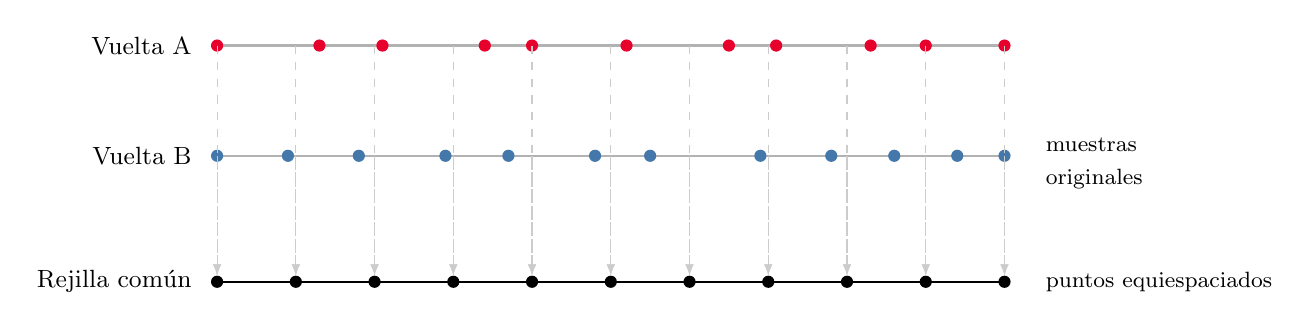
\begin{tikzpicture}[x=1cm,y=1cm,>=latex]
    \definecolor{syncred}{HTML}{E8002D}
    \definecolor{syncblue}{HTML}{4477AA}
    % Vuelta A (muestras irregulares)
    \node[anchor=east] at (-0.2,2) {\small Vuelta A};
    \draw[thick,gray!60] (0,2) -- (10,2);
    \foreach \x in {0,1.3,2.1,3.4,4.0,5.2,6.5,7.1,8.3,9.0,10}
      \fill[syncred] (\x,2) circle (2.2pt);
    % Vuelta B (muestras irregulares, distintas)
    \node[anchor=east] at (-0.2,0.6) {\small Vuelta B};
    \draw[thick,gray!60] (0,0.6) -- (10,0.6);
    \foreach \x in {0,0.9,1.8,2.9,3.7,4.8,5.5,6.9,7.8,8.6,9.4,10}
      \fill[syncblue] (\x,0.6) circle (2.2pt);
    % Rejilla comun
    \node[anchor=east] at (-0.2,-1) {\small Rejilla común};
    \draw[thick] (0,-1) -- (10,-1);
    \foreach \x in {0,1,2,3,4,5,6,7,8,9,10}{
      \fill[black] (\x,-1) circle (2.2pt);
      \draw[gray!40,dashed,->] (\x,2) -- (\x,-0.92);
      \draw[gray!40,dashed,->] (\x,0.6) -- (\x,-0.92);
    }
    \node[anchor=west,align=left] at (10.4,0.5)
      {\footnotesize muestras\\\footnotesize originales};
    \node[anchor=west] at (10.4,-1) {\footnotesize puntos equiespaciados};
  \end{tikzpicture}
  \caption{Sincronización de dos vueltas por interpolación sobre una rejilla de distancia común. Las muestras originales de cada vuelta, registradas en posiciones distintas, se remuestrean sobre puntos equiespaciados compartidos que permiten compararlas directamente.}
  \label{fig:sincronizacion}
\end{figure}

\section{Estado del arte}
El análisis de telemetría en competición ha seguido históricamente dos caminos paralelos, el de las herramientas profesionales, propietarias y de acceso restringido a los equipos, y el del ecosistema abierto construido por la comunidad a partir de los datos que las organizaciones publican. Esta sección recorre ambos, sitúa las iniciativas académicas más relevantes y concluye con un análisis comparativo que justifica el hueco que viene a cubrir este proyecto.
\subsection{Herramientas profesionales}
El primer camino lo ocupan las herramientas profesionales que los propios equipos y organizadores emplean. Son soluciones potentes pero propietarias, de coste elevado y acceso restringido, lo que las sitúa fuera del alcance del aficionado. Esta sección repasa las más representativas.

\subsubsection{McLaren Applied ATLAS}
McLaren Applied es el proveedor exclusivo de la unidad de control electrónico estándar (SECU por sus siglas en inglés) de todos los equipos de Fórmula 1 desde 2008, contrato que renovó hasta 2030.
Esta posición convierte su plataforma de análisis ATLAS (\textit{Advanced Telemetry Linked Acquisition System}), en el estándar de \textit{facto} del \textit{paddock}, todos los monoplazas generan datos a través del mismo hardware, lo que facilita la adopción de un entorno común \cite{atlas}.

\medskip
\noindent ATLAS captura, distribuye y visualiza datos procedentes de los sistemas de control del monoplaza. La telemetría opera en modo "ráfaga" enviando así todos los datos almacenados de una vuelta al pasar por un punto concreto. De igual manera incorpora modelos de aprendizaje para predecir
degradación del neumático, consumo de combustible y eventos de carrera a medida que avanza la sesión. En 2023 McLaren Applied integró la base de datos de series temporales KX para añadir capacidades de consulta analítica sobre datos de telemetría en tiempo real.

\noindent ATLAS es el software comercial cerrado, disponible únicamente bajo contrato con McLaren Applied. No existe versión libre ni documentación pública de sus interfaces. Su coste y sus requisitos de infraestructura lo sitúan fuera del alcance del aficionado promedio.

\subsubsection{AWS F1 Insights}
Desde 2018 Amazon Web Services es el socio oficial de nube e inteligencia artificial de la Fórmula 1 \cite{awsf1}. La colaboración se materializa en dos planos.

\noindent El plano más visible son las \textbf{F1 Insights}: infografías generadas por IA que aparecen durante las retransmisiones televisivas. El catálogo supera los veinticuatro indicadores, entre los que se encuentran
\textit{Battle Forecast} (cuántas vueltas hasta que alcanza la distancia de adelantamiento), \textit{Undercut Threat} (análisis de la estrategia de parada en boxes), \textit{Tyre Performance} (estimación de ángulos de deslizamiento y energía de desgaste), \textit{Corner Analysis} (desglose de la curva en 4 fases) o \textit{Driver Performance} (evaluación del piloto sobre siete métricas).
En 2025 se añadió \textit{Track Pulse}, basado en IA generativa (Amazon Bedrock), que sintetiza la situación a tiempo real en pista para los equipos de producción televisiva. La Figura~\ref{fig:aws} muestra un ejemplo del indicador \textit{Battle Forecast} emitido durante una retransmisión.

\begin{figure}[ht]
  \centering
  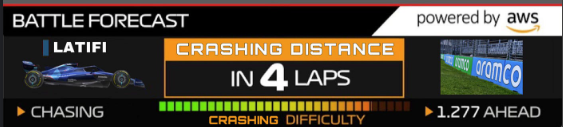
\includegraphics[width=0.8\textwidth]{AWS}
  \caption{Ejemplo de gráfico \textit{Battle Forecast} de AWS F1 Insights emitido durante una carrera.}
  \label{fig:aws}
\end{figure}

\medskip
\noindent Sin embargo estas herramientas no son un sistema de análisis para los equipos sino un producto de entretenimiento para el espectador. Cada equipo recibe únicamente los datos de su propio coche a través de canales propietarios
y AWS procesa los datos agregados de los monoplazas con fines de difusión. Existe una arquitectura llamada Amazon S3 que cuenta con décadas de datos históricos, redes neuronales y \textit{pipelines} de ML. Esta arquitectura es de gran interés técnico, pero no expone ninguna
interfaz accesible al exterior.

\subsubsection{Otras plataformas comerciales: MoTeC y Bosch Motorsport}
\noindent MoTeC es una empresa australiana con amplia presencia en categorías inferiores a la F1 (Fórmula 2, Fórmula 3, resistencia, turismos). Su software de análisis i2 permite superposición de vueltas, histogramas, análisis de presión de freno y comparación de aceleración en base tiempo y distancia.
La versión estándar se incluye con la compra de hardware MoTeC (Registradores como el C70 o C80, cuyo coste asciende a varios miles de euros). La versión Pro requiere licencia adicional. En la Fórmula 1 MoTeC no compite directamente con ATLAS
dada la relación contractual de McLaren Applied con la FIA, pero la filosofía analítica es un referente conceptual en el campo.

\noindent Bosch Motorsport ofrece registradores de datos profesionales con software de análisis propio. El acceso está en ambos casos vinculado a la adquisición de hardware profesional.

\subsubsection{Datos oficiales de la Fórmula 1}
\noindent La Fórmula 1 publica datos de la sesión a través de una API de sincronización en directo que no requiere autenticación, no hay documentación oficial de dicha API. El contenido disponible incluye
tiempos de vuelta, sectores, compuesto del neumático, posición GPS simplificada y telemetría básica del piloto. Todos estos datos son propiedad de Formula One World Championship Limited y su uso comercial requiere licencia.
La aplicación oficial F1 y la plataforma F1TV ofrecen una interfaz de consumo de estos datos, no una herramienta de análisis.

\subsection{Ecosistema de código abierto}
Frente a las soluciones propietarias, en torno a los datos que la Fórmula 1 publica ha surgido un ecosistema de herramientas de código abierto. Estas no acceden a la telemetría completa de los equipos, sino al subconjunto de datos públicos, pero lo hacen de forma gratuita y documentada. A continuación se describen las principales fuentes de datos sobre las que se sustenta este ecosistema, incluida la que emplea este trabajo.
\subsubsection{FastF1}
\noindent FastF1 es la biblioteca de Python de referencia para el acceso y análisis de datos históricos de Fórmula 1 \cite{fastf1}. Desarrollada y mantenida por la comunidad bajo el pseudónimo de theOehrly, alcanza las 5.000 estrellas en GitHub y es la herramienta más utilizada en proyectos de análisis amateur y académico.

\noindent FastF1 unifica el acceso a dos fuentes: la API no oficial de sincronización en directo de la F1 y Jolpica-F1 para resultados históricos. Toda la información se devuelve como DataFrame de Pandas extendido con métodos específicos del dominio. Las capacidades principales incluyen tiempos de vuelta y sector,
telemetría básica del coche correlacionada con posición X/Y en la pista, datos meteorológicos, información de compuestos y un sistema de caché en disco que evita descargas.

\noindent La cobertura histórica es fiable desde la temporada 2019, con disponibilidad parcial desde 2018. Las limitaciones más significativas son la dependencia de una API no oficial que F1 podría modificar o restringir sin previo aviso.
FastF1 es una librería de acceso y preprocesado, no ofrece ninguna interfaz de usuario.

\subsubsection{De Ergast a Jolpica-F1}
\noindent Durante más de una década, la Ergast Motor Racing Developer API \cite{ergast} fue la fuente canónica de datos históricos de F1 para la comunidad, ofreciendo resultados y clasificaciones desde la temporada 1950 a través de una API REST documentada y gratuita. Ergast fue deprecada a finales de 2024.

\noindent Como respuesta, la comunidad desarrolló Jolpica-F1 \cite{jolpica}, una reimplementación compatible con los mismos \textit{endpoints}, mantenida de forma voluntaria y con cobertura desde 1950 hasta el presente.
FastF1 migró a Jolpica como \textit{backend} histórico. La deprecación de Ergast ilustra la fragilidad estructural de toda la cadena de datos abiertos en la que se apoya este trabajo: la disponibilidad de los datos depende de decisiones de terceros sin compromisos de continuidad.

\subsubsection{OpenF1 API}
\noindent OpenF1 \cite{openf1} es una API REST gratuita y de código abierto que proporciona telemetría en tiempo real e histórica. Expone dieciocho \textit{endpoints} con documentación pública completa: telemetría del coche a 3,7 Hz, posición en pista cada cuatro segundos, tiempos y datos del pit lane, mensajes de dirección, registros de radio y datos meteorológicos.

\noindent La cobertura histórica se limita a partir de 2023, lo que supone una desventaja frente a FastF1. La versión gratuita cubre todos los \textit{endpoints} históricos sin autenticación, el acceso en directo requiere una suscripción.
Esta API representa la evolución más documentada del ecosistema abierto, aunque su cobertura temporal reducida limita su uso para análisis multitemporada.

\subsection{Proyectos y Herramientas de la comunidad}
Sobre las fuentes de datos anteriores, la comunidad ha construido un conjunto de proyectos y herramientas de visualización. Su alcance y madurez son muy variados, desde cuadernos de análisis hasta dashboards interactivos constituyendo el contexto más cercano a este proyecto.
\subsubsection{Dashboards basados en FastF1}
\noindent \textbf{F1Dash (FraserTarbet)} \cite{f1dash} es un dashboard analítico interactivo construido con Python y Plotly sobre FastF1. Proporciona competitividad por vuelta, comparación de trazas, telemetría superpuesta entre pilotos y un panel de condiciones de pista filtrable por equipo, piloto y compuesto, como se aprecia en la Figura~\ref{fig:f1dash}.
Es el referente más cercano a TALOS dentro del ecosistema abierto aunque no cubre la totalidad de módulos que este trabajo implementa.

\noindent \textbf{F1-Tempo} \cite{f1tempo} es una herramienta web de comparación de telemetría construida con React y TypeScript sobre FastF1. Permite superponer la telemetría de distintos pilotos, sesiones o años, e incluye un mapa del circuito coloreado según qué piloto fue más rápido en cada punto y la selección automática de las vueltas más rápidas. Es un buen ejemplo de herramienta puesto que resuelve muy bien una única tarea (la comparación de trazas vuelta a vuelta), pero su alcance se limita a esa función y no aborda el análisis de estrategia, la cronología de eventos, la dinámica vehicular ni la clasificación de estilos que sí cubre este trabajo.

\noindent \textbf{f1-dash (slowlydev)} es un dashboard en tiempo real construido con Next.js que consume la API oficial. Proporciona la clasificación en directo, estado de neumáticos y tiempos de sector durante las sesiones. Su orientación es la monitorización en directo, no el análisis post-sesión.

\noindent En GitHub, el \textit{topic} fastf1 agrupa decenas de repositorios con cuadernos Jupyter para análisis de temporada. La mayoría son análisis puntuales no mantenidos y sin interfaz de usuario.

\begin{figure}[ht]
  \centering
  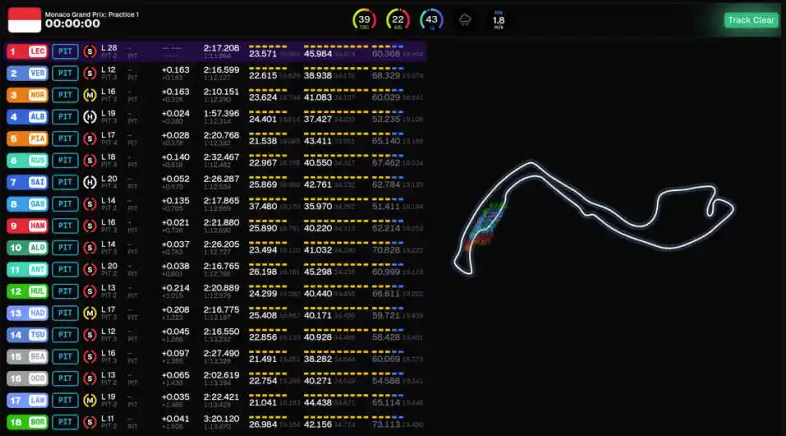
\includegraphics[width=\textwidth]{F1Dash}
  \caption{Interfaz de F1Dash, dashboard de telemetría en tiempo real basado en FastF1.}
  \label{fig:f1dash}
\end{figure}

\subsubsection{Grafana y el \textit{stack} de monitorización genérico}
\noindent Grafana es una plataforma de observabilidad de código abierto orientada a series temporales. Existe un caso en el blog de Grafana Labs \cite{grafanaf1} en el que se implementa un \textit{stack} de telemetría F1 utilizando el \textit{feed} UDP del videojuego \textit{F1 2020} de Codemasters como fuente de datos, Apache Kafka como broker de mensajería, InfluxDB como base de datos y Grafana como visualización, desplegado sobre Kubernetes.

\noindent El resultado es impresionante a nivel técnico pero conceptualmente alejado del problema que abarca este trabajo: Los datos provienen de una simulación y la infraestructura necesaria requiere conocimientos significativos. Grafana no incorpora ningún concepto del dominio.

\subsubsection{Herramientas BI genéricas: Tableau y Power BI}
\noindent Las principales plataformas de \textit{Business Intelligence} cuentan con adopción documentada en el análisis deportivo de élite para carga de entrenamiento, prevención de lesiones y análisis táctico. En F1, McLaren ha reconocido el uso de Tableau junto a Python y MATLAB como herramientas complementarias.

\noindent Sin embargo, ni Tableau ni Power BI incorporan conectores nativos para las APIs anteriormente mencionadas, por lo que el acceso a telemetría requiere pipelines de preprocesado en Python. Las licencias tienen coste.
Estas herramientas están optimizadas para métricas de negocio y agregaciones, el análisis de señales de telemetría es un caso de uso atípico que no explotan de forma natural.

\subsection{Investigación académica}
\noindent El interés académico y universitario por el análisis de datos ha crecido notablemente desde la disponibilidad de la API FastF1. Los trabajos existentes se agrupan en dos líneas claramente diferenciadas: investigación en predicción y optimización de estrategia, y proyectos de visualización e interfaz de usuario. Ninguno de los trabajos combina ambas líneas de forma integrada.

\subsubsection{Investigación Internacional en estrategia y predicción}
\noindent \textbf{Bekker y Lotz (2009)} \cite{bekker2009} publicaron uno de los primeros modelos formales de simulación de estrategia de carrera mediante simulación de eventos discretos, validado sobre tres Grandes Premios de 2005. Operan sin datos reales de telemetría puesto que no existían APIs en ese entonces y recurren a modelos paramétricos.
Representa el punto de partida de la investigación operativa aplicada a la Fórmula 1.
\medskip
\noindent \textbf{Heilmeier et al. (2020)} \cite{heilmeier2020} proponen el \textit{Virtual Strategy Engineer}, un sistema basado en redes neuronales artificiales (FFNN + LSTM) entrenado sobre datos de temporadas 2014-2019 para tomar decisiones de pit stop y selección de compuesto.
Es uno de los primeros trabajos que aborda el problema de estrategia de carrera desde el aprendizaje profundo y ha servido de referencia para trabajos posteriores.
\medskip
\noindent \textbf{Aversa, Cabantous y Haefliger (2018)} \cite{aversa2018} analizan en el \textit{Journal of Strategic Information Systems} el Gran Premio de Abu Dabi 2010, donde Ferrari tomó una decisión de estrategia subóptima que costó el campeonato a Alonso a pesar de disponer de herramientas DSS avanzadas.
Los autores identifican tres fuentes de fallo: la naturaleza situada de la toma de decisiones, la cognición distribuida y la performatividad del DSS. Este marco teórico justifica el diseño de herramientas transparentes y no prescriptivas como TALOS.
\medskip
\noindent \textbf{Aguad y Thraves (2024)} \cite{aguad2024} formulan la estrategia de pit stops en F1 como un juego de Stackelberg de suma cero con programación dinámica, modelizando la interacción estratégica entre equipos ante eventos imprevistos como el \textit{safety car}. Publicado en el \textit{European Journal of Operational Research}, representa la aplicación más rigurosa de la teoría de juegos a la estrategia de carreras.
\medskip
\noindent En el ámbito del aprendizaje por refuerzo, \textbf{Thomas et al. (2025)} \cite{thomas2025rl} presentan en ACM SAC un sistema de RL explicable (\textit{Explainable Reinforcement Learning}) para estrategia de carrera, introduciendo árboles de decisión. Probado sobre el GP de Baréin 2023.

\subsubsection{Trabajos de fin de grado}
El panorama de TFG/TFM en España sobre análisis de Fórmula 1 reproduce a escala universitaria la misma dicotomía que se observa en la investigación.

\noindent \textbf{Morán Montero (Universidad de Extremadura, 2022)} \cite{moranextremadura2022} desarrolla dos modelos de aprendizaje automático, incluye un clasificador de circuitos y una red neuronal para predecir resultados de carrera. El enfoque es modelado offline sin incluir ninguna interfaz de usuario.
No utiliza FastF1 ya que este trabajo es anterior a su adopción generalizada.

\noindent \textbf{Cid Espeso (Universidad Politécnica de Madrid, 2023)} \cite{cidespeso2023} construye un dashboard interactivo de seguimiento de carreras utilizando Dash Plotly como framework, FastF1 y OpenF1 para los datos.
Usa MongoDB como caché de sesión. Cubre estrategias de \textit{pitstop}, ritmo de carrera y comparativas. Es el referente más cercano a este proyecto entre los TFGs españoles. Comparte el enfoque de interfaz con datos reales. La principal diferencia es la integración
de clasificadores y módulos de ML además del análisis de fuerzas G.

\noindent \textbf{Latorre Castelltort (Universitat de Barcelona, 2025)} \cite{latorreub2025} desarrolla una aplicación de análisis histórico y en tiempo real con un chatbot de lenguaje natural para el soporte al usuario.

\subsubsection{Análisis comparativo y posicionamiento de la aplicación}
\noindent El recorrido por herramientas profesionales, ecosistema \textit{open-source}, proyectos comunitarios y trabajos académicos permite trazar con precisión el lugar que este proyecto ocupa. La tabla \ref{tab:comparativa} resume los atributos de cada alternativa.

\begin{table}[ht]
  \centering
  \caption{Comparativa de herramientas de análisis de telemetría de Fórmula 1.}
  \label{tab:comparativa}
  \small
  \begin{tabularx}{\textwidth}{l c c c X c}
    \toprule
    \textbf{Herramienta} & \textbf{Gratuita} & \textbf{F1} & \textbf{UI} & \textbf{Cobertura} & \textbf{Barrera} \\
    \midrule
    McLaren ATLAS      & No  & Sí & Sí & Completa (privada) & Restringida \\
    AWS F1 Insights    & No  & Sí & No & Live (broadcast)   & Sin API \\
    MoTeC i2           & No  & No & Sí & Hardware propio    & Alta \\
    FastF1             & Sí  & Sí & No & 2019--hoy          & Baja \\
    OpenF1             & Parcial & Sí & No & 2023--hoy      & Baja \\
    F1Dash             & Sí  & Sí & Sí & FastF1             & Baja \\
    Grafana + Kafka    & Sí  & No & Sí & Simulación         & Muy alta \\
    Tableau / Power BI & No  & No & Sí & Requiere pipeline  & Media \\
    TFG Morán (2022)   & Sí  & Sí & No & Batch offline      & Media \\
    TFG Cid (2023)     & Sí  & Sí & Sí & 2019--hoy          & Baja \\
    \midrule
    \textbf{TALOS}     & \textbf{Sí} & \textbf{Sí} & \textbf{Sí} & \textbf{2018--hoy} & \textbf{Baja} \\
    \bottomrule
  \end{tabularx}
\end{table}

\chapter{Metodología, Decisiones de análisis y diseño del sistema}

\section{Metodología}
\noindent El desarrollo de este proyecto ha seguido un enfoque iterativo e incremental adoptando prácticas habituales en proyectos de software ágil sin ceñirse a un marco estricto de trabajo.
Este modelo resulta adecuado para proyectos explorativos en los que los requisitos evolucionan a medida que se profundiza en el dominio del problema.
\subsection{Modelo de desarrollo}
\noindent El desarrollo se organizó en iteraciones cortas centradas en la entrega de funcionalidad completa por módulo. Cada iteración seguía un ciclo de cuatro fases:
análisis de la funcionalidad, diseño de la solución, implementación y validación del resultado mediante tests unitarios y conocimiento del dominio.
Al finalizar cada iteración el módulo quedaba integrado en la aplicación principal y disponible para su uso y posterior revisión.
Este enfoque permitió detectar y corregir problemas de forma temprana, permitió pivotar el diseño de módulos posteriores a partir de la experiencia acumulada en los anteriores.
\subsection{Seguimiento con el tutor}
\noindent A lo largo del proyecto se mantuvieron reuniones con el tutor. Cada reunión tenía como objetivo revisar el avance desde el último encuentro, validar las decisiones técnicas y establecer los objetivos y mejoras para la siguiente iteración.
Este canal de comunicación permitió mantener la coherencia del proyecto y reorientar el trabajo cuando fue necesario.
\subsection{Gestión de tareas}
\noindent Para la gestión de tareas se utilizó \textbf{GitHub Projects}, configurado como tablero \textit{kanban} con cinco columnas: \textit{backlog}, \textit{ToDo}, \textit{In Progress}, \textit{Done} y \textit{Testing}. Cada tarea correspondía a un módulo, funcionalidad o conjunto de módulos durante el desarrollo.
Además, las diferentes tareas fueron divididas en épicas que corresponden al marco general de la funcionalidad: Algoritmos, Diseño, \textit{Backend}, Interfaz gráfica, Pruebas/validación y Entregables. La Figura~\ref{fig:githubprojects} muestra el estado del tablero durante el desarrollo.

\begin{figure}[ht]
  \centering
  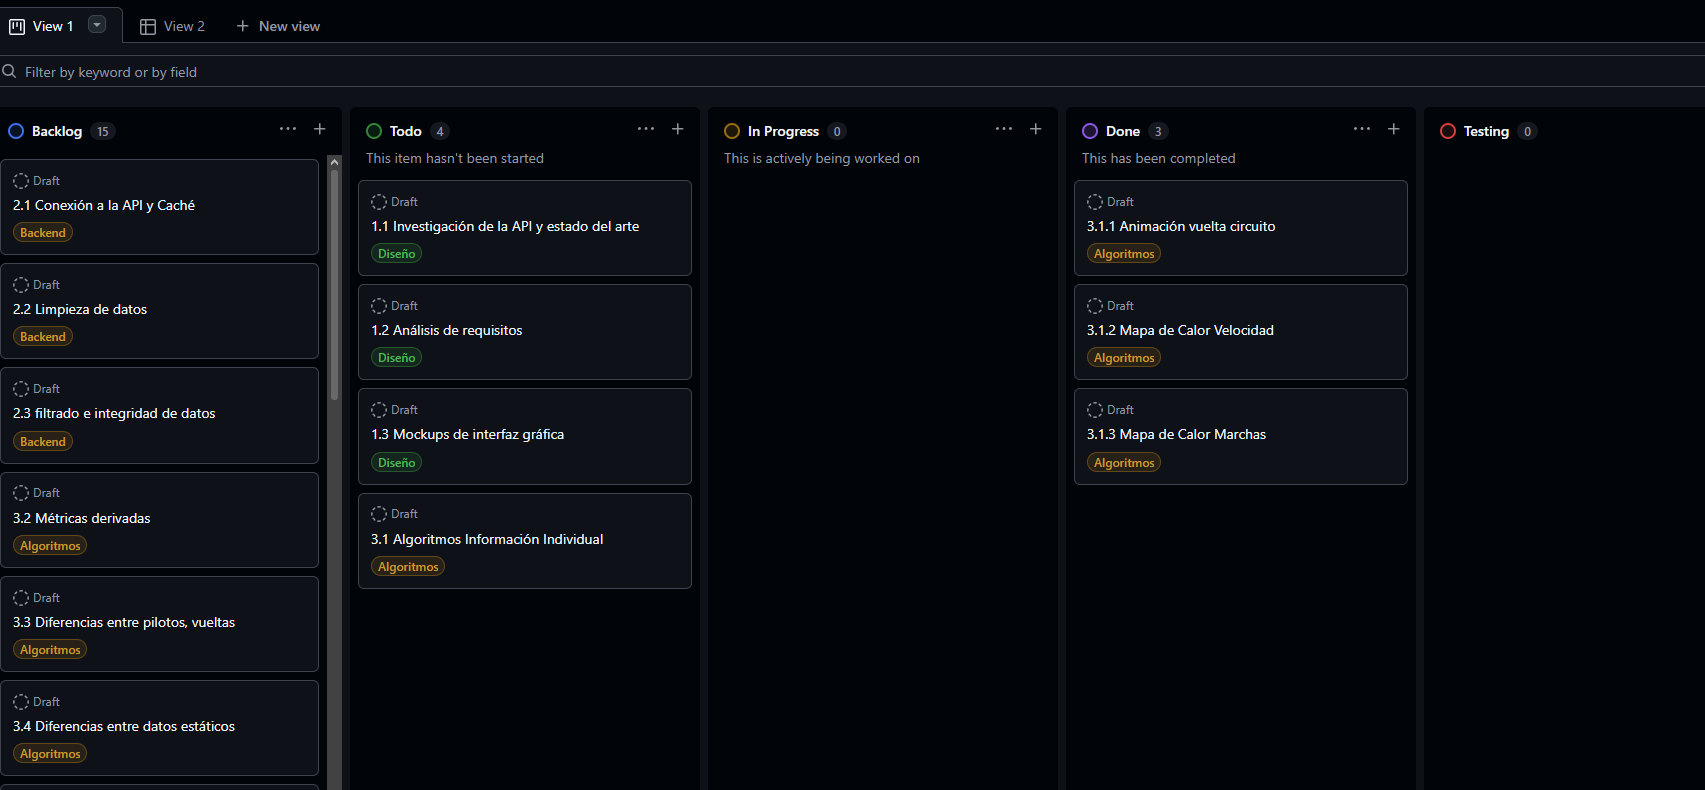
\includegraphics[width=0.8\textwidth]{GitHubProjects.png}
  \caption{Ejemplo de gráfico \textit{GitHub Projects} durante la realización del trabajo.}
  \label{fig:githubprojects}
\end{figure}

\subsection{Control de versiones}
\noindent El código fuente se gestionó con \textit{Git} y se alojó en un repositorio de \textit{GitHub}. Se trabajó sobre la rama principal main, realizando commits asociados a funcionalidades o conjunto de estas.
El repositorio es público y está disponible en \url{https://github.com/hgdario/f1-telemetry-dss}. El proceso de instalación y puesta en marcha se detalla en el Apéndice~\ref{app:instalacion}.

\subsection{Planificación temporal}
\noindent La tabla \ref{tab:temporalizacion} recoge la distribución de horas por fase establecidas en el anteproyecto.
\begin{table}[ht]
  \centering
  \caption{Temporización del proyecto por fases.}
  \label{tab:temporalizacion}
  \small
  \begin{tabularx}{\textwidth}{X c}
    \toprule
    \textbf{Fase} & \textbf{Horas} \\
    \midrule
    Planificación y estado del arte                          & 30 \\
    Diseño de la arquitectura y datos                        & 55 \\
    Desarrollo de algoritmos de análisis y métricas          & 40 \\
    Programación de la lógica para el cálculo de métricas   & 35 \\
    Implementación del dashboard y controladores             & 30 \\
    Integración de visualizaciones dinámicas                 & 35 \\
    Elaboración de pruebas y validación                      & 35 \\
    Elaboración de memoria técnica                           & 36 \\
    \midrule
    \textbf{Total}                                           & \textbf{296} \\
    \bottomrule
  \end{tabularx}
\end{table}

\section{Análisis de requisitos}
Como se indicó en el anteproyecto de este proyecto se ha realizado un trabajo profundo de análisis de requisitos. Esta investigación sobre el diseño de la aplicación nos deja con los siguientes requisitos funcionales y no funcionales:
A cada requisito se le ha asignado una prioridad basada en la importancia dentro del dominio del problema y la dificultad/interés técnico que profesa.
La tabla \ref{tab:rf} representa los requisitos funcionales del sistema mientras que la \ref{tab:rnf} los no funcionales.
\medskip
\begin{xltabular}{\textwidth}{l l X l}
  \caption{Requisitos funcionales del sistema.} \label{tab:rf} \\
  \toprule
  \textbf{ID} & \textbf{Nombre} & \textbf{Descripción} & \textbf{Prioridad} \\
  \midrule
  \endfirsthead
  \multicolumn{4}{r}{\small\textit{Continúa en la página siguiente}} \\
  \endfoot
  \bottomrule
  \endlastfoot
    RF01 & Selección de temporada   & El sistema permite seleccionar año & Alta \\
    \hline
    RF02 & Selección de sesión   & El sistema permite seleccionar GP y sesión eligiendo entre \textit{Free Practice}, \textit{Qualy} o carrera. Si lo hubiera se incluyen los \textit{sprints} & Alta \\
    \hline
    RF03 & Carga de telemetría   & Descargar y subir a caché los datos completos de la sesión que se descarga & Alta \\
    \hline
    RF04 & Resumen de sesión   & El primer módulo del sistema, mostrar circuito, clasificación y datos generales & Baja \\
    \hline
    RF05 & Cronología de Eventos   & Línea temporal de actividad durante la sesión, balance de adelantamientos y tiempo de paradas en \textit{boxes} & Media \\
    \hline
    RF06 & Mapa de Velocidad   & Mapa de calor del circuito según la velocidad & Baja \\
    \hline
    RF07 & Mapa de Marchas   & Mapa de calor del circuito según la marcha del piloto & Baja \\
    \hline
    RF08 & Estrategia de neumáticos   & Diagrama de Gantt indicando los compuestos usados. Se debe indicar la combinación más usada & Media \\
    \hline
    RF09 & Telemetry Trace   & Canales de telemetría completos de una vuelta a elegir & Alta \\
    \hline
    RF10 & Resumen del piloto  & KPIs, sectores y stints de cada piloto & Baja \\
    \hline
    RF11 & Panel de equipo & Panel con sendos pilotos e información para un equipo & Alta \\
    \hline
    RF12 & Comparativa de sesión   & Canales de telemetría multi-piloto & Media \\
    \hline
    RF13 & Animación circuito   & Animación del coche por el circuito sincronizada a tiempo & Alta \\
    \hline
    RF14 & Vuelta Ideal   & Vuelta óptima dividiendo el circuito en microsectores, permite filtrado por equipo & Media \\
    \hline
    RF15 & Coche Fantasma   & Comparación de dos monoplazas en una animación conjunta & Alta \\
    \hline
    RF16 & Diagrama G-G  & Análisis de fuerzas G del trazado y Diagrama G-G teórico de la vuelta & Alta \\
    \hline
    RF17 & Carga aerodinámica   & Estimación teórica del downforce & Baja \\
    \hline
    RF18 & Carga por rueda   & Mapa de calor del circuito según la carga del neumático & Alta \\
    \hline
    RF19 & Clasificador de tipo de vuelta   & Uso de \textit{K-means} para agrupar en \textit{clusters} los tipos de vuelta & Alta \\
    \hline
    RF20 & Clasificador de estilo de conducción   & Uso de \textit{K-means} para agrupar en \textit{clusters} los tipos de conducción basado en tipo de vuelta y telemetría de vuelta & Alta \\
    \hline
    RF21 & Clasificador de tipo de circuito   & Uso de \textit{K-means} para agrupar en \textit{clusters} los tipos de circuito basado en fuerzas G & Alta \\
\end{xltabular}

\begin{table}[ht]
  \centering
  \caption{Requisitos no funcionales del sistema.}
  \label{tab:rnf}
  \small
  \begin{tabularx}{\textwidth}{l l X l}
    \toprule
    \textbf{ID} & \textbf{Nombre} & \textbf{Descripción} & \textbf{Prior.} \\
    \midrule
    RNF01 & Rendimiento   & Carga reducida mediante caché de disco y en memoria & Alta \\
    \hline
    RNF02 & Usabilidad    & Interfaz navegable sin conocimientos técnicos & Alta \\
    \hline
    RNF03 & Reproducibilidad & Instalable con un único bat desde el repositorio & Alta \\
    \hline
    RNF04 & Ejecutabilidad & Ejecutable con un único bat desde el repositorio & Alta \\
    \hline
    RNF05 & Independencia & Sin APIs de pago, servidores propios ni BBDD externas & Alta \\
    \hline
    RNF06 & Compatibilidad & Ejecutable en cualquier SO con Python 3.10+ & Media \\
    \hline
    RNF07 & Mantenibilidad & Módulos independientes fácilmente ampliables & Media \\
    \hline
    RNF08 & Código abierto & Código fuente público y libre para su uso. & Media \\
    \bottomrule
  \end{tabularx}
\end{table}

\section{Tecnologías empleadas}
El desarrollo se ha llevado íntegramente en \textbf{Python}, aprovechando el ecosistema de bibliotecas científicas y de visualización que lo convierten en el entorno natural para proyectos de este estilo. La interfaz de usuario ha sido construida sobre \textbf{Streamlit}~\cite{streamlit}, un \textit{framework} de código abierto que permite desarrollar aplicaciones web interactivas orientadas al análisis de datos y sin separar el \textit{backend} del \textit{frontend}. Los gráficos e interacciones visuales han sido implementados con \textbf{Plotly}~\cite{plotly}, que proporciona visualizaciones integrables de forma nativa en Streamlit.

\noindent El acceso a los datos de la Fórmula 1 se realiza a través de \textbf{FastF1}, una biblioteca de código abierto que unifica el acceso a la API oficial de la Fórmula 1 y a la API histórica de Ergast, incorporando además un sistema de caché local que reduce los tiempos de carga en sesiones repetidas. El procesamiento y la manipulación de los datos se apoyan en \textbf{Pandas}~\cite{pandas} y \textbf{NumPy}~\cite{numpy}, mientras que el filtrado de señales de telemetría utiliza la implementación del filtro Savitzky-Golay disponible en \textbf{SciPy}~\cite{scipy}. Los módulos de aprendizaje automático se implementan con \textbf{scikit-learn}~\cite{sklearn} para el entrenamiento y \textbf{NumPy}. El control de versiones y el repositorio del proyecto se alojan en \textbf{GitHub}. El entorno de desarrollo integrado utilizado ha sido \textbf{Visual Studio Code} y la elaboración de diagramas y esquemas de la memoria se ha realizado con \textbf{draw.io}. La Figura~\ref{fig:tecnologias} recoge el conjunto de tecnologías empleadas.

\begin{figure}[ht]
  \centering
  
\includegraphics[height=1.2cm]{logos/python}
  \hspace{0.4cm}
  
\includegraphics[height=1.2cm]{logos/streamlit}
  \hspace{0.4cm}
  
\includegraphics[height=1.2cm]{logos/fastf1}
  \hspace{0.4cm}
  
\includegraphics[height=1.2cm]{logos/plotly}
  \hspace{0.4cm}
  
\includegraphics[height=1.2cm]{logos/pandas}
  \hspace{0.4cm}
  
\includegraphics[height=1.2cm]{logos/numpy}
  \hspace{0.4cm}
  
\includegraphics[height=1.2cm]{logos/scipy}
  \hspace{0.4cm}
  
\includegraphics[height=1.2cm]{logos/sklearn}
  \hspace{0.4cm}
  
\includegraphics[height=1.2cm]{logos/GitHub}
  \hspace{0.4cm}
  
\includegraphics[height=1.2cm]{logos/vscode}
  \hspace{0.4cm}
  
\includegraphics[height=1.2cm]{logos/drawio}
  \caption{Tecnologías utilizadas en el desarrollo de TALOS.}
  \label{fig:tecnologias}
\end{figure}

\section{Diseño del sistema}
A la hora de planear el diseño del sistema se han valorado alternativas en casi todos los ámbitos del desarrollo desde el \textit{framework} de interfaz hasta las decisiones de gráficos y clasificadores.
En esta sección recorreremos de forma granular las decisiones de diseño más importantes que se han tomado durante la planificación y desarrollo de la aplicación.
TALOS se organiza en módulos de análisis agrupados en cuatro categorías que siguen una progresión de lo general a lo específico, tal y como se muestra en la Tabla~\ref{tab:modulos}.

\begin{table}[H]
  \centering
  \caption{Organización de módulos de TALOS por categoría.}
  \label{tab:modulos}
  \small
  \begin{tabularx}{\textwidth}{l X}
    \toprule
    \textbf{Categoría} & \textbf{Módulos} \\
    \midrule
    Información de Sesión  & Resumen de sesión, Cronología de eventos, Estrategia de neumáticos \\
    Análisis de Piloto     & Resumen del piloto, Mapa de velocidad, Mapa de marchas, Telemetry trace \\
    Comparativas           & Panel de equipo, Comparativa de sesión, La vuelta ideal, Coche fantasma \\
    Dinámica Vehicular     & Diagrama G-G, Carga aerodinámica, Mapa de carga por rueda \\
    \bottomrule
  \end{tabularx}
\end{table}

\noindent La Figura~\ref{fig:arquitectura} muestra el flujo de navegación entre vistas y la relación de componentes de manera ilustrada para facilitar la comprensión.

\begin{figure}[H]
  \centering
  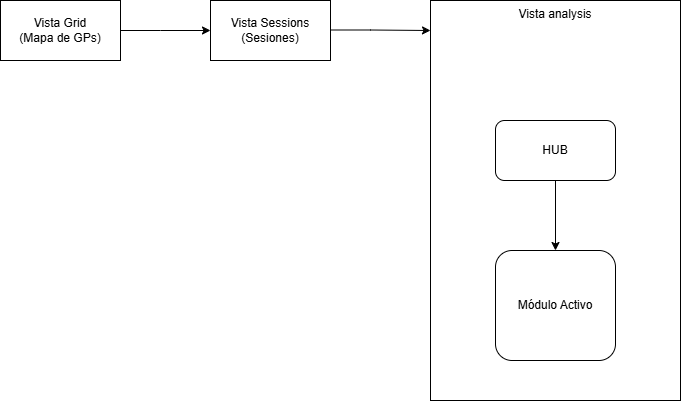
\includegraphics[width=\textwidth]{diagrama_arquitectura}
  \caption{Diagrama de navegación y arquitectura de vistas de TALOS.}
  \label{fig:arquitectura}
\end{figure}
\noindent Sigue una arquitectura de \textit{Single Page Application} construida sobre Streamlit. La navegación se articula en tres vistas secuenciales: la vista en \lstinline{grid} (Figura~\ref{fig:vista_grid}), que representa el mapa mundial interactivo que aloja los Grandes Premios de la temporada seleccionada.
La vista \lstinline{sessions} (Figura~\ref{fig:vista_session}), donde el usuario elige el tipo de sesión a analizar y por último el \lstinline{analysis} (Figura~\ref{fig:vista_hub}) que aloja el hub de módulos y el módulo activo en cada momento. La transición entre estas vistas se gestiona mediante la función \lstinline{go()} de \lstinline{session_loader.py}, que actualiza el estado de sesión y fuerza la re-ejecución del script.
\begin{figure}[H]
  \centering
  \begin{subfigure}{0.32\textwidth}
    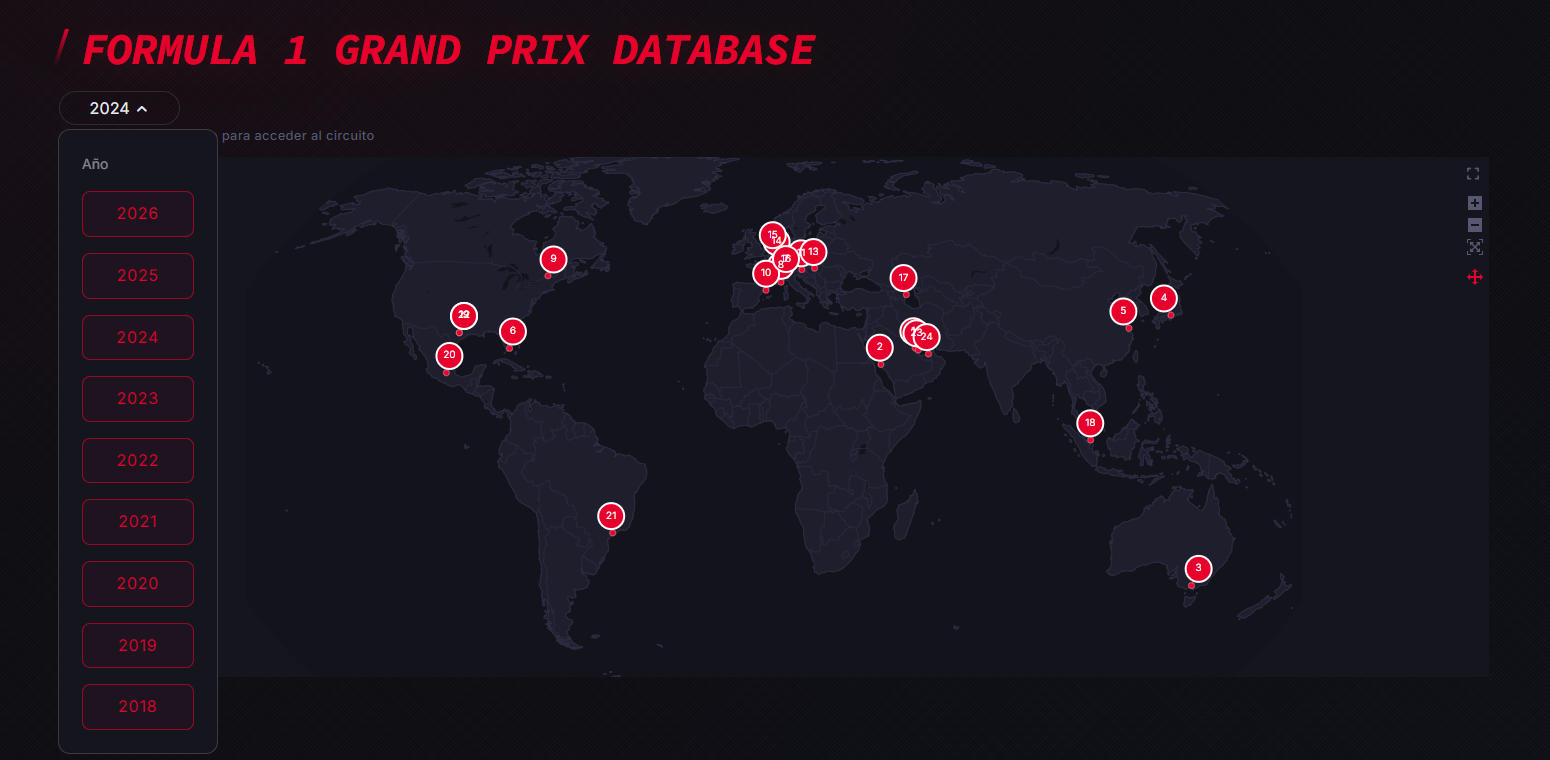
\includegraphics[width=\textwidth]{grid}
    \caption{Vista \textit{Grid}}
    \label{fig:vista_grid}
  \end{subfigure}\hfill
  \begin{subfigure}{0.32\textwidth}
    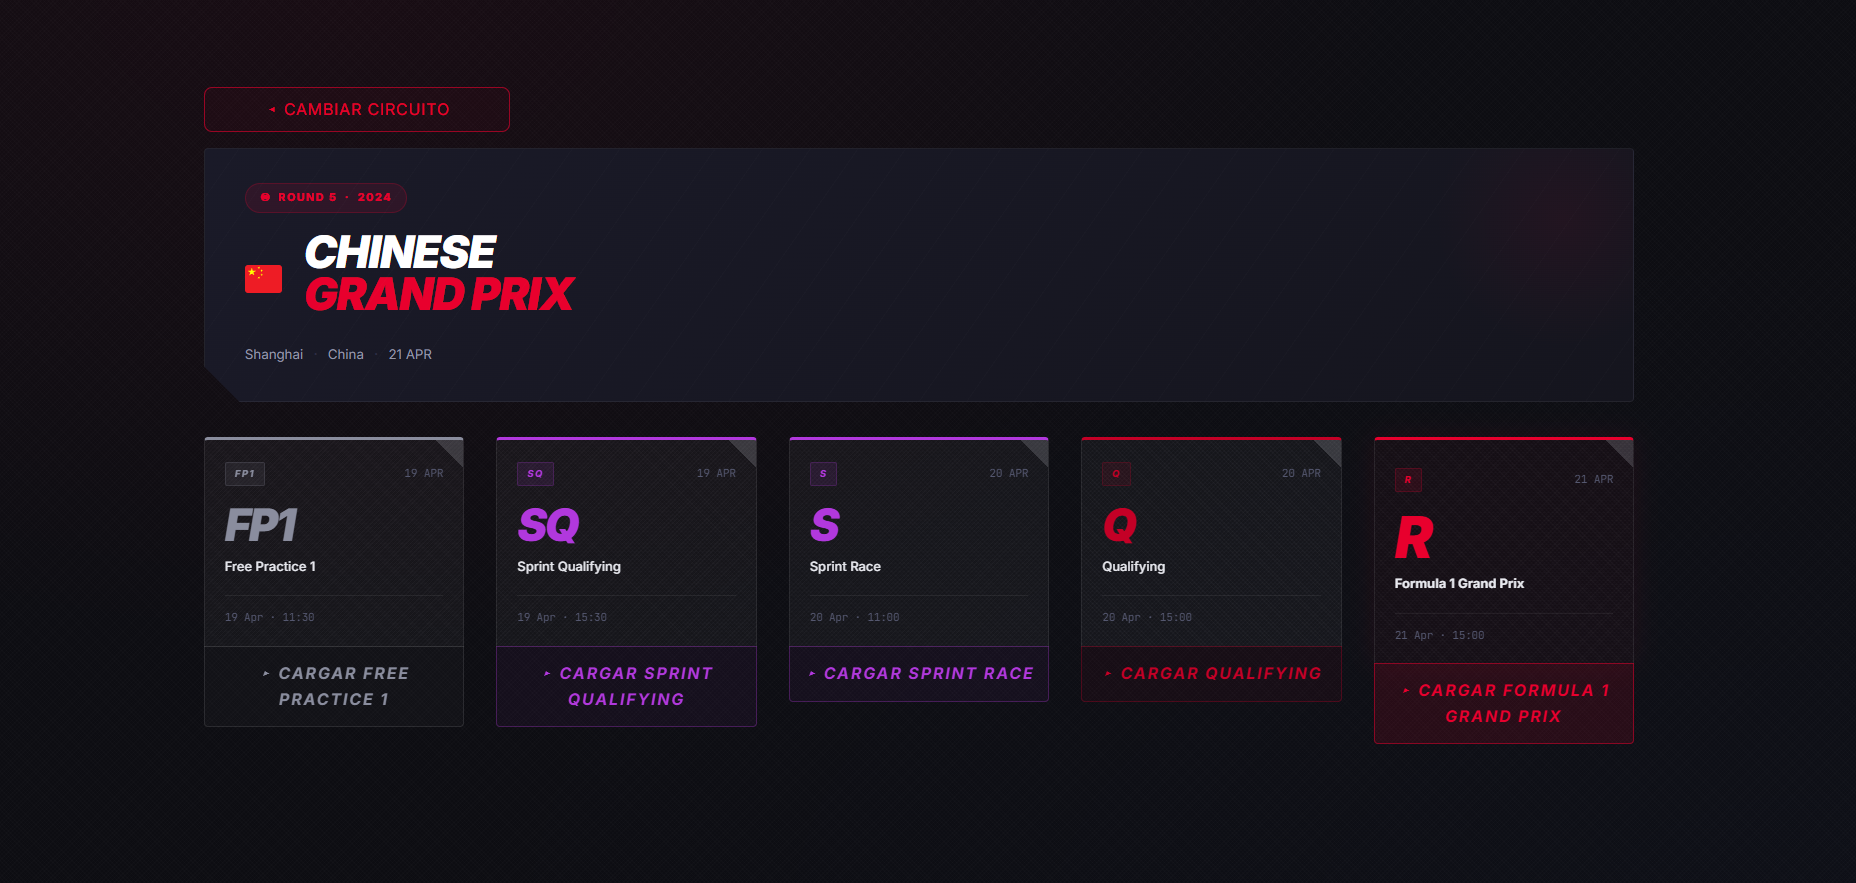
\includegraphics[width=\textwidth]{session}
    \caption{Vista \textit{Sessions}}
    \label{fig:vista_session}
  \end{subfigure}\hfill
  \begin{subfigure}{0.32\textwidth}
    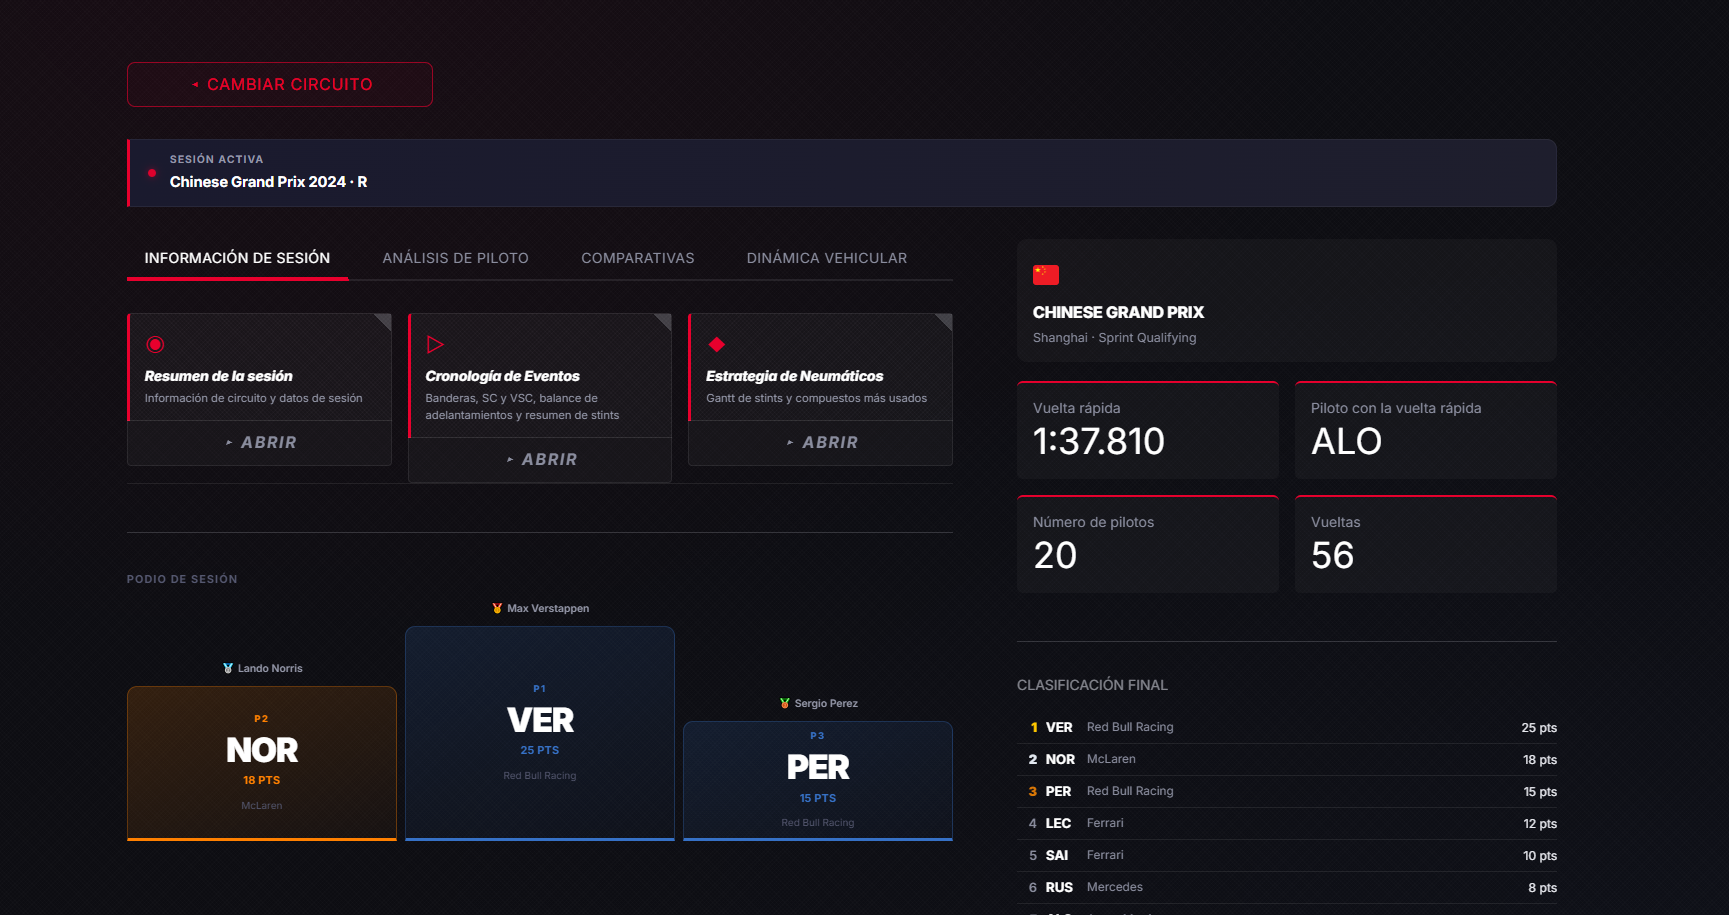
\includegraphics[width=\textwidth]{hub}
    \caption{Vista \textit{Analysis}}
    \label{fig:vista_hub}
  \end{subfigure}
  \caption{Las tres vistas secuenciales de la navegación de TALOS: el mapa mundial de Grandes Premios (\textit{Grid}), la selección de sesión (\textit{Sessions}) y el hub de módulos de análisis (\textit{Analysis}).}
  \label{fig:vistas}
\end{figure}

\subsection{FastF1 sobre otras alternativas}
Como hemos comentado antes la API oficial de la Fórmula 1 requiere suscripción de pago volviéndola incompatible con el enfoque \textit{open-source}. Otras alternativas como OpenF1 solo tiene cobertura desde 2023 por lo que cuenta con muchos canales de telemetría incompletos. FastF1 es la solución gratuita con más cobertura, es una API que está documentada y unifica la API oficial y datos históricos con la integración de
Ergast y Jolpica, contando con una comunidad muy activa en GitHub. El sistema de caché de disco es un factor diferencial con el objetivo de reducir descargas repetidas sin aportar nada adicional.

\subsection{Streamlit para interfaz}
Para la interfaz se ha usado Streamlit, un \textit{framework} de ciencia de datos que permite construir la aplicación íntegramente en Python sin depender de una separación entre \textit{backend} y \textit{frontend}.
El modelo de re-ejecución completa en cada interacción encaja bien con los dashboards de análisis donde el usuario cambia parámetros y espera nuevos resultados. Tiene una curva baja de aprendizaje lo que permitió centrarse en la lógica de análisis en lugar de la infraestructura web.
Streamlit permite la ejecución en local mediante un único comando sin configurar servidores, puertos ni builds.
Sin embargo, Streamlit cuenta con un menor control sobre la interfaz gráfica del proyecto permitiendo una limitada personalización visual. Esto pudo compensarse con inyecciones de CSS desde un archivo aparte de assets.
Se valoraron otras alternativas como Dash (más flexible) y Flask+JS sin embargo es mucho más complejo.

\subsection{Estado de la sesión}
Streamlit no tiene estado persistente entre re-ejecuciones salvo \lstinline{st.session_state}.
Se centraliza en esta sesión todo lo que las vistas requieren compartir como año seleccionado, evento, objeto a tratar o módulo activo. Esto permite que independientemente de dónde se encuentre el usuario en la aplicación se compartan los datos más importantes
entre módulos. \lstinline{session_loader.py} es el único punto que escribe el estado inicial evitando inconsistencias. Si un módulo necesita información de la sesión lee el estado en lugar de pedirla de nuevo.

\subsection{Caché de dos niveles}
Se usa un primer nivel de caché en disco. FastF1 serializa los datos de cada sesión que ha sido cargada en disco, cuando se trate de cargar la misma sesión no hace ninguna petición de red lo que permite a la aplicación funcionar offline.
En un segundo nivel se utiliza \lstinline{@st.cache_data} en \lstinline{session_loader.py} lo que permite mantener el calendario y la sesión en RAM durante la ejecución así no necesita traer de disco cada interacción. Sin este sistema de doble caché, cada cambio de módulo relanzaría la descarga completa de telemetría.

\subsection{Módulos independientes entre sí}
Se ha tratado de reducir lo máximo posible el acoplamiento entre módulos permitiendo así añadir, modificar o eliminar un módulo sin riesgo de romper los demás.
La mayoría de los módulos importan solo de \lstinline{session_loader} y librerías externas. Hay un router principal \lstinline{app.py} que lanza la aplicación y actúa como orquestador. Este \textit{router} lee \lstinline{active_module} del estado y llama a la función \lstinline{render_*()} correspondiente.
Esto permite que los módulos puedan desarrollarse y probarse independiente y en paralelo.

\subsection{K-Means pre-entrenado}
A la hora de realizar los clasificadores se ha optado por tener pre-entrenados estos. Entrenar los clasificadores en tiempo real requeriría descargar y procesar varias temporadas de datos resultando inviable en tiempo de respuesta.
Los scripts de entrenamiento están separados de la parte de producción de modo que ni se importan ni ejecutan. El modelo entrenado es cargado en runtime de forma rápida, es esta separación la que permite re-entrenar los clasificadores con datos nuevos sin necesidad de tocar el código de la aplicación.

\subsection{Interfaz Visual}
El diseño visual adopta una estética oscura inspirada en la identidad gráfica de la Fórmula 1. Consta de una paleta basada en tonos de rojo \#E8002D sobre fondos oscuros. Uso de la tipografía Titillium Web habitual en la comunicación del deporte (además de Inter y JetBrains Mono). El objetivo era que la herramienta resultara familiar desde el primer vistazo a cualquier aficionado promedio, sin instrucciones necesarias.

\noindent Antes de comenzar la implementación se elaboraron \textit{mockups} de las vistas principales usando draw.io, estos bocetos recogían la disposición general de los elementos aunque algunos acabaron pivotando en el layout. Han servido como referencia visual temprana durante el desarrollo.
\noindent El funcionamiento completo de la interfaz y la descripción de cada uno de sus módulos se recogen en el Apéndice~\ref{app:usuario}.
\chapter{Implementación}
\noindent Los capítulos anteriores han descrito qué es lo que hace la aplicación y por qué se tomaron determinadas decisiones de diseño. Este capítulo da el paso siguiente explicando cómo se han materializado todas las decisiones de diseño en código.
Se mostrarán fragmentos más representativos de determinadas decisiones técnicas en lugar de mostrar el código completo, que se encuentra en el repositorio.

\noindent Como se detalló en el apartado de tecnologías, el sistema se ha construido en Python, empleando Streamlit y FastF1 como fuente de datos, Plotly para la visualización y CSS y HTML para la interfaz de usuario.
A lo largo del capítulo se recorren los distintos subsistemas de la herramienta: Primero la estructura general del código y la organización de los módulos, la gestión de estado y caché, procesamiento de telemetría y cálculo de variables físicas y los clasificadores no supervisados. Por último se detallará el sistema visual que da su identidad a la aplicación.

\section{Estructura del código}
El código de la aplicación se organiza en dos raíces claramente diferenciadas siendo \texttt{src/} y \texttt{research/}. La primera, contiene el código en producción: todo lo que se ejecuta cuando un usuario lanza la aplicación. La segunda, agrupa los \textit{scripts} de exploración, contando con versiones antiguas de módulos ya implementados o nuevos módulos en progreso de implementar. Esta carpeta tiene como intención el tener un entorno de investigación para un futuro desarrollo o mejora de lo ya programado.
Esta carpeta también contiene los \textit{scripts} de entrenamiento que se ejecutan una sola vez y de forma aislada, sin formar parte de la herramienta desplegada. Esta separación es deliberada de modo que se mantienen los prototipos fuera del código de producción evitando que la lógica experimental contamine la aplicación y deja claro qué es lo que se ejecuta en cada contexto.

\noindent El listado \ref{lst:tree} muestra la estructura de directorios del proyecto, tal y como se encuentra en el repositorio.

\begin{lstlisting}[caption={Estructura de directorios del proyecto.},label=lst:tree,numbers=none]
TALOS/
|-- src/                        # Codigo de produccion
|   |-- app.py                  # Punto de entrada y enrutado
|   |-- session_loader.py       # Estado, carga y cache
|   |-- ui_assets.py            # CSS, JS y utilidades de color
|   |-- Circuit2d.py            # Renderizado 2D del trazado
|   |-- CircuitClassifier.py    # Clasificador de circuitos (K-Means)
|   |-- DriverStyleClassifier.py# Clasificador de estilo de piloto (K-Means)
|   |-- LapTypeClassifier.py    # Clasificador de tipo de vuelta (K-Means)
|   |-- informacion_sesion/     # Resumen, cronologia, estrategia
|   |-- analisis_piloto/        # Mapas, telemetria, resumen de piloto
|   |-- comparativas/           # Head-to-head, vuelta ideal, coche fantasma
|   |-- dinamica_vehicular/     # Diagrama G-G, aero, carga por rueda
|   |-- assets/                 # Logos de equipos y siluetas
|   \-- data/                   # Firmas de pilotos precalculadas
|-- research/                 # Entrenamiento offline (scrapers + K-Means)
|   \-- data/                 # Datasets de caracteristicas
|-- requirements.txt          # Dependencias con versiones fijadas
|-- install.bat / start.bat   # Instalacion y arranque (Windows)
\-- f1_cache/                 # Cache de FastF1 (excluida de git)
\end{lstlisting}

\noindent El punto de entrada a la aplicación es \texttt{app.py}, que actúa como orquestador y no contiene lógica de análisis. Su responsabilidad se limita a coordinar definiendo la navegación, importando los estilos globales, inicializa el estado de sesión y delega cada vista al módulo correspondiente. El catálogo de funcionalidades se declara en un solo diccionario \texttt{NAV}, que constituye la fuente de verdad sobre qué módulos existen, a qué categoría pertenecen y con qué icono se presentan.
Gracias a este registro incorporar una nueva funcionalidad se reduce a añadir una entrada en el \texttt{NAV} y su correspondiente \textit{import}, sin tocar la lógica del enrutado manteniendo al mínimo el acoplamiento entre componentes.
El listado \ref{lst:nav} muestra la separación en categorías dentro del \texttt{NAV}.
\begin{lstlisting}[style=python,caption={Registro declarativo de la navegación en \texttt{app.py}.},label=lst:nav]
NAV = {
    "Información de Sesión": [
        ("Resumen de la sesión",    "...", "Información de circuito y datos de sesión"),
        ("Cronología de Eventos",   "...", "Banderas, SC y VSC, balance de adelantamientos y resumen de stints"),
        ("Estrategia de Neumáticos","...", "Gantt de stints y compuestos más usados"),
    ],
    "Análisis de Piloto": [
        ("Resumen del Piloto",      "...", "Síntesis de sesión: KPIs, sectores, stints y distribución"),
        ("Mapa de Velocidad",       "...", "Circuito coloreado por velocidad (km/h)"),
        ("Mapa de Marchas",         "...", "Circuito coloreado por marcha seleccionada"),
        ("Telemetry Trace",         "...", "Canales de telemetría, circuito animado y estilo de conducción del piloto"),
    ],
    "Comparativas": [
        ("Panel de Equipo",         "...", "Análisis intra-equipo"),
        ("Comparativa de Sesión",   "...", "Overlays multi-piloto sobre la misma vuelta"),
        ("La Vuelta Ideal",         "...", "Microsectores óptimos de toda la parrilla y filtrado por equipos"),
        ("Coche Fantasma",          "...", "Animación 2D de persecución entre pilotos"),
    ],
    "Dinámica Vehicular": [
        ("Diagrama G-G",            "...", "Círculo de tracción y envolvente de Gs"),
        ("Carga Aerodinámica",      "...", "Estimación teórica de carga aerodinámica"),
        ("Mapa de Carga por Rueda", "...", "Distribución de carga por eje y temperatura de frenos"),
    ],
}

# Lista aplanada de módulos, usada por el enrutado
MODULE_KEYS = [m for cat in NAV.values() for m, _, _ in cat]
\end{lstlisting}

\noindent Los módulos se reparten en cuatro paquetes correspondientes a las cuatro categorías presentadas: \texttt{informacion\_sesion/}, \texttt{analisis\_piloto/}, \texttt{comparativas/} y \texttt{dinamica\_vehicular/}. Esta correspondencia directa facilita localizar cualquier funcionalidad basándonos en la categoría que el usuario ve. 
Todos los módulos comparten además una función pública llamada \texttt{render\_*()} que recibe la sesión ya cargada y se encarga de construir su vista. Esta uniformidad hace que, desde el orquestador, todos los módulos sean intercambiables ya que responden a la misma firma.

\noindent En la raíz de \texttt{src/} quedan únicamente los componentes compartidos por toda la aplicación siendo \texttt{session\_loader.py} que centraliza la gestión del estado, la carga de sesiones y la caché, mientras que \texttt{ui\_assets.py} concentra los estilos y las utilidades de color. Junto a ellos residen los clasificadores, que se implementan como utilidades en lugar de como vistas ya que no aparecen en el \texttt{NAV} anteriormente mencionado y son los propios módulos los que invocan a los clasificadores.

\noindent El repositorio se ha preparado pensando en la reproducibilidad. El archivo \texttt{requirements.txt} fija las versiones exactas de las dependencias, y los \textit{scripts} de instalación automatizan la instalación y el arranque en sistemas Windows. La caché de telemetría de FastF1 se almacena en \texttt{f1\_cache/} un directorio excluido del control de versiones ya que no tiene lugar versionar datos descargables que se regeneran la primera vez que se solicita la sesión.

\section{Modelo y Acceso a datos}\label{sec:datos}
Obtenemos todos los datos de una única fuente: \textbf{FastF1}, una biblioteca Python que combina la API de Fórmula 1, la telemetría oficial y datos de Ergast.
No hay base de datos propia ni scraping manual, FastF1 abstrae la descarga y parseo y devuelve \textit{DataFrames} de Pandas listos para operar.

\subsection{Origen y naturaleza de datos}
FastF1 es la única fuente, expone los datos de telemetría a 3,7 Hz aproximadamente (muestreo variable según el canal) y los eventos de \textit{timing} (banderas, stints, tiempos de vuelta, posiciones) en un \textit{DataFrame} de Pandas. Se accede a todo a través de una sesión.
Una sesión es una carrera, clasificación, libre o \textit{sprint} de un gran premio y año concretos. La carga de estos eventos se dispara con \texttt{fastf1.get\_session(year, gp, ses)} seguido de un \texttt{.load()}. Este último es la operación red + parseo a JSON que la caché de la aplicación hace opaca para el usuario.

\subsection{Modelo Jerárquico de datos}
FastF1 estructura una sesión en tres niveles anidados que son recorridos en el mismo orden:
\texttt{Session} expone \texttt{session.results} que nos otorga la clasificación final y \texttt{session.weather\_data} que nos da la temperatura, lluvia y datos meteorológicos.

\noindent Los canales de telemetría vienen con \textit{timestamps} relativos al inicio de vuelta, no con distancia recorrida.
El listado \ref{lst:fastf1schema} es un ejemplo de cómo vienen los datos dentro de FastF1.
\begin{lstlisting}[caption={Campos representativos de cada nivel de datos de FastF1.},label=lst:fastf1schema,numbers=none]
# session.laps  -- DataFrame, una fila por vuelta
{ "Driver": "VER", "LapNumber": 42, "LapTime": "0:01:31.456",
  "Compound": "MEDIUM", "TyreLife": 8, "Stint": 2 }

# lap.get_telemetry().add_distance()  -- ~3.7 Hz, una fila por muestra
{ "Speed": 312.4, "RPM": 11823, "nGear": 7,
  "Throttle": 100.0, "Brake": false, "DRS": 12,
  "X": -2134.5, "Y": 891.2, "Distance": 1456.3 }

# session.results  -- una fila por piloto
{ "Abbreviation": "VER", "GridPosition": 1,
  "ClassifiedPosition": "1", "Status": "Finished" }

# session.weather_data  -- una fila por muestra meteorologico
{ "AirTemp": 27.4, "TrackTemp": 41.1,
  "Humidity": 38.0, "WindSpeed": 2.1 }
\end{lstlisting}

\subsection{Patrón de preparación}
Cada módulo sigue la misma secuencia para ir del objeto sesión a los datos a visualizar:

\noindent 1. \textbf{Selección de vuelta} - \texttt{laps.pick\_drivers(driver)} filtra las vueltas por piloto.

\noindent 2. \textbf{Expansión de telemetría} - \texttt{lap.get\_telemetry()} devuelve el \textit{DataFrame} de alta frecuencia para esa vuelta

\noindent 3. \textbf{Añadir distancia} - \texttt{.add\_distance()} integra la velocidad para generar una columna de Distancia que se convierte en el eje X natural de todos los trazados de telemetría.

\noindent 4. \textbf{Saneamiento por canal} - \texttt{series.dropna()} descarta muestras ausentes a raíz de fallos o eventos de la carrera como accidentes o banderas rojas.

\noindent El listado \ref{lst:tel} muestra este patrón tal y como aparece en \texttt{Telemetrytrace.py}, la función encargada de descargar la telemetría de una vuelta concreta:

\begin{lstlisting}[style=python,caption={Patrón de acceso a telemetría en \texttt{Telemetrytrace.py}.},label=lst:tel]
def _extract_telemetry(session: Session, driver: str,
                       lap_number: int) -> Optional[pd.DataFrame]:
    """
    Descarga la telemetría de una vuelta específica y añade columna Distance.
    Retorna DataFrame o None si falla.
    """
    try:
        laps = session.laps.pick_drivers(driver)
        lap: Lap = laps[laps["LapNumber"] == lap_number].iloc[0]
        tel = lap.get_telemetry().add_distance()
        if tel.empty:
            return None
        return tel
    except Exception as e:
        st.warning(f"[!] No se pudo cargar la telemetría: {e}")
        return None
\end{lstlisting}

\subsection{Caché}
Cargar la sesión tarda entre 2 y 15 segundos según la sesión y la conexión. Sin caché, cada \textit{rerun} de Streamlit relanzaría la descarga. Con \texttt{@st.cache\_data}, la primera carga persiste en memoria del servidor y por tanto cada \textit{rerun} posterior es instantáneo.
El módulo \texttt{session\_loader.py} centraliza tanto la lógica de caché como el estado de la aplicación. \texttt{init\_session\_state()} registra con \texttt{setdefault} todas las claves que la app necesita, de modo que los reruns no pisan el estado ya cargado.
\texttt{load\_schedule(year)} utiliza una caché con \texttt{ttl=3600} porque el calendario puede actualizarse a lo largo de la temporada.
\texttt{load\_f1\_session(year, gp, ses)} utiliza una caché sin TTL porque una sesión histórica es inmutable; la clave de caché es la tupla \texttt{(year, gp, ses)}.

\noindent Por último, \texttt{require\_session()} actúa de \textit{guard} en cada módulo: si no hay sesión cargada muestra el aviso y aborta el render
como puede observarse en el listado \ref{lst:session}.
\begin{lstlisting}[style=python,caption={Gestión de estado y caché en \texttt{session\_loader.py}.},label=lst:session]
import streamlit as st
import pandas as pd
import fastf1


# --- ESTADO ------------------------------------------------------------------

def init_session_state() -> None:
    """Inicializa todas las claves de session_state que usa la app."""
    st.session_state.setdefault("view",            "grid")   # grid | sessions | analysis
    st.session_state.setdefault("selected_year",   2024)
    st.session_state.setdefault("selected_event",  None)
    st.session_state.setdefault("f1_session",      None)
    st.session_state.setdefault("session_loaded",  False)
    st.session_state.setdefault("session_label",   "")
    st.session_state.setdefault("active_module",   None)     # None = Hub
    st.session_state.setdefault("corners",         False)


# --- CACHÉ ------------------------------------------------------------------

@st.cache_data(show_spinner=False, ttl=3600)
def load_schedule(year: int) -> pd.DataFrame:
    """Calendario FastF1 del año (sin testing)."""
    return fastf1.get_event_schedule(year, include_testing=False)


@st.cache_data(show_spinner=False)
def load_f1_session(year: int, gp: str, ses: str):
    """Carga (y cachea) una sesión FastF1. Cachea por (year, gp, ses)."""
    s = fastf1.get_session(year, gp, ses)
    s.load()
    return s


# --- HELPERS -----------------------------------------------------------------

def require_session() -> bool:
    """Devuelve False y muestra aviso si no hay sesión cargada."""
    if not st.session_state.get("session_loaded", False):
        st.warning("Carga una sesión desde el panel lateral para continuar.")
        return False
    return True


def go(view: str) -> None:
    """Cambia la vista activa y fuerza rerun."""
    st.session_state["view"] = view
    st.rerun()
\end{lstlisting}

\section{Información de sesión}
La primera de las cuatro categorías funcionales ofrece la visión panorámica de un Gran Premio. A diferencia de las otras categorías, aquí el trabajo consiste en leer los datos
que FastF1 entrega y presentarlos de forma que se entiendan con un simple vistazo. La categoría agrupa tres módulos que sirven como resumen de lo que ha ocurrido en un Gran Premio:
el resumen de la sesión, cronología de eventos y estrategia de neumáticos.

\subsection{Resumen de la sesión}
El módulo \texttt{SessionSummary.py} construye la portada de la carrera, reuniendo en una sola pantalla la información contextual requerida para comprender el Gran Premio. 
Incluye una cabecera con el nombre del evento y el año, un mapa del trazado del circuito, las condiciones meteorológicas (En el caso de haber cargado una carrera serán relativas a otros fines de semana) y un bloque de estadísticas de la sesión.

\noindent El mapa del circuito no es una imagen cargada, es una gráfica mostrada en tiempo real a partir de las coordenadas de posición \texttt{X} e \texttt{Y} contenidas en la telemetría de la vuelta más rápida de la sesión, siguiendo el patrón de acceso a datos descrito en la sección anterior.
La propia traza GPS del coche define la silueta del circuito. El bloque meteorológico promedia los registros de \texttt{session.weather\_data} para mostrar la temperatura del aire, asfalto y humedad siendo estas tres variables que condicionan directamente el rendimiento de los neumáticos y, por tanto, la estrategia.
Para añadir un mayor marco contextual, si el evento elegido es de tipo carrera se mostrará una comparación con el resto de fines de semana para poder situar el evento entre los más cálidos o fríos del año. Esta distinción se hace mediante la lectura de \texttt{track\_temp\_by\_weekend.csv} localizado en la carpeta de \texttt{data/}.

\noindent Finalmente, este resumen incorpora lo que en la herramienta se denomina \textit{ADN del circuito}: una clasificación automática que sitúa el trazado dentro de una familia de circuitos con características físicas similares. Esta clasificación se apoya
en un modelo de aprendizaje no supervisado cuya construcción y validación se detallan en la sección \ref{sec:clasificadores}, por lo que aquí únicamente se señala su punto de integración. La Figura~\ref{fig:resumen} muestra el aspecto de esta vista.

\begin{figure}[H]
  \centering
  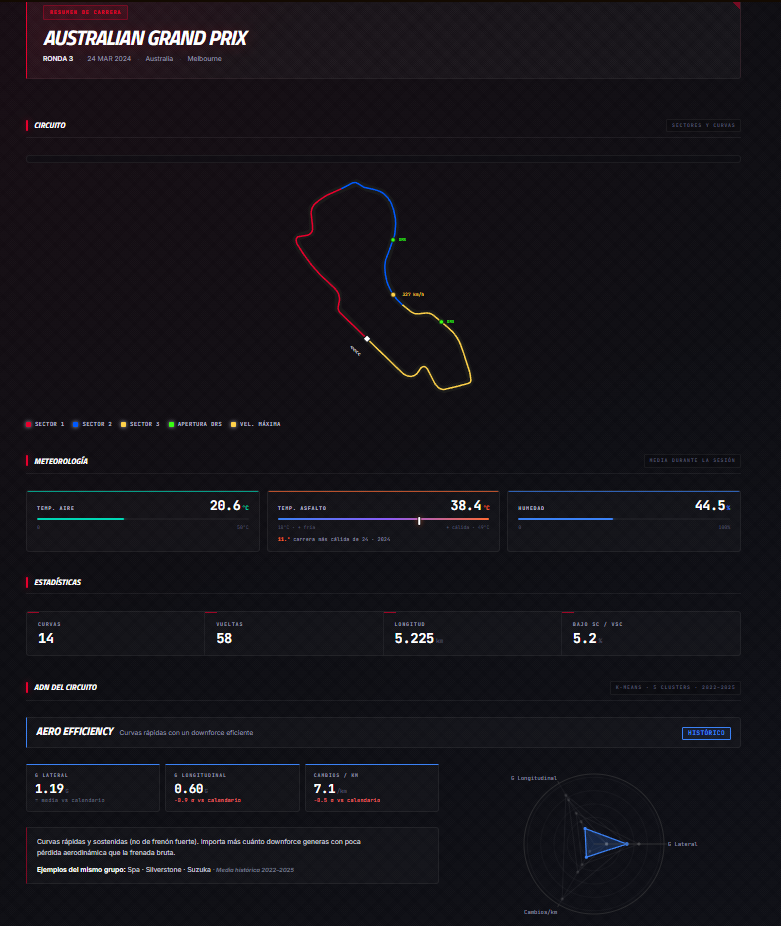
\includegraphics[width=\textwidth]{resumen.png}
  \caption{Vista de Resumen de la sesión: mapa del circuito dibujado desde la telemetría, condiciones meteorológicas y estadísticas de la carrera.}
  \label{fig:resumen}
\end{figure}

\subsection{Cronología de Eventos}
Una carrera de Fórmula 1 rara vez transcurre sin interrupciones. Cuando se produce un accidente o aparece un peligro en pista, la dirección de carrera neutraliza total o parcialmente la competición mediante banderas y coches de seguridad.
El módulo \texttt{SessionTimeLine.py} reconstruye esa secuencia de incidentes a lo largo del tiempo y la presenta como una línea temporal legible.

\noindent El reto técnico está en el origen de los datos. FastF1 entrega estos eventos como una secuencia de códigos numéricos en el campo \texttt{session.track\_status}, un \texttt{1} significa pista despejada, un \texttt{4} indica un \textit{Safety Car} (Un coche real que encabeza al grupo a una velocidad reducida para parar la carrera), un \texttt{6} corresponde al
\textit{Virtual Safety Car} (Un equivalente electrónico, sin coche físico), un \texttt{5} indica una bandera roja (Sesión suspendida) y así sucesivamente. El módulo traduce cada uno de estos códigos a un evento comprensible asociando a cada código una etiqueta, color y descripción. De este modo un dato pensado para una máquina se convierte en información que cualquier aficionado interpreta sin esfuerzo.

\noindent A esta línea temporal se añaden dos análisis complementarios, balance de adelantamientos, que es obtenido comparando la posición de salida con la final, ambas disponibles en \texttt{session.results}. El segundo es un resumen de los \textit{stints} de cada piloto.
Se entiende por \textit{stint} cada tanda de vueltas consecutivas realizadas con un mismo juego de neumáticos. Es decir, el tramo de carrera entre dos paradas en \textit{boxes}. La Figura~\ref{fig:timeline} muestra esta vista de cronología.

\begin{figure}[H]
  \centering
  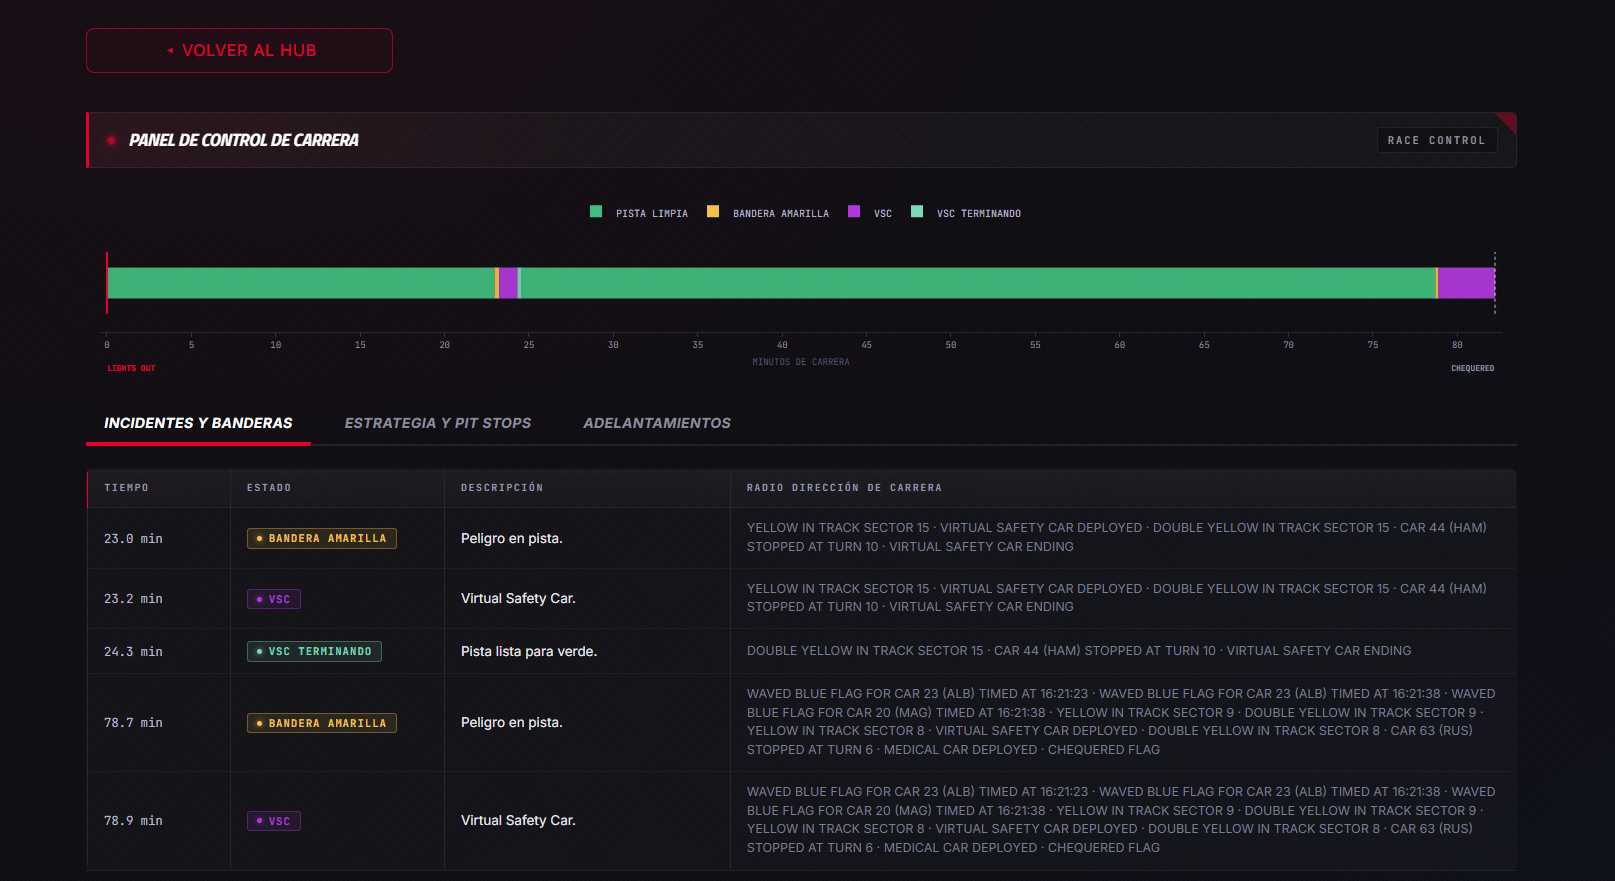
\includegraphics[width=\textwidth]{timeline.png}
  \caption{Vista de Cronología de Eventos: reconstrucción de la secuencia de banderas, \textit{Safety Car} y \textit{VSC} a lo largo de la sesión a partir de los códigos de \texttt{track\_status}.}
  \label{fig:timeline}
\end{figure}

\noindent A modo de ejemplo, la Figura~\ref{fig:russell} recoge el accidente que originó uno de estos eventos de neutralización en la cronología de la Figura~\ref{fig:timeline}.
\begin{figure}[H]
  \centering
  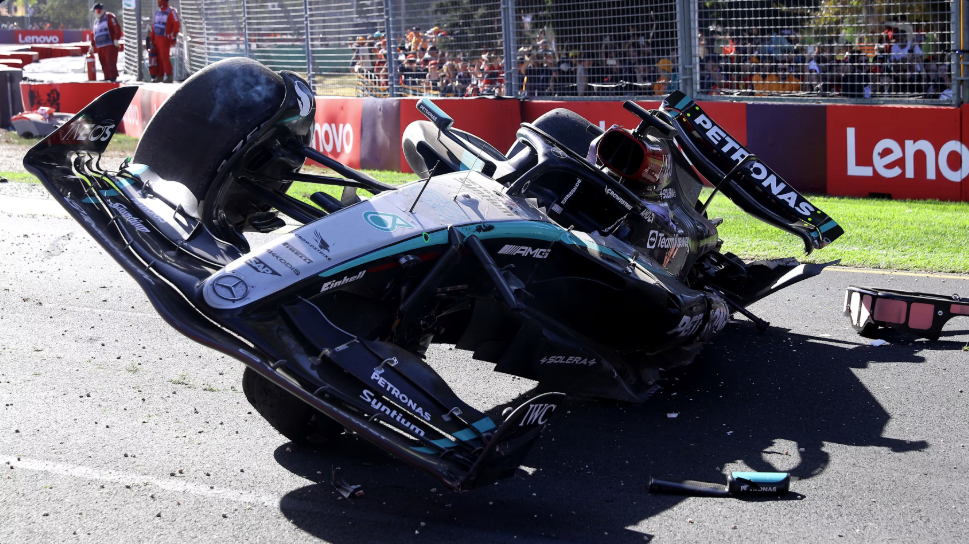
\includegraphics[width=0.7\textwidth]{russell_australia2024.png}
  \caption[Accidente de Russell, GP de Australia 2024]{Accidente de George Russell en la última vuelta del Gran Premio de Australia 2024, que neutralizó la carrera con bandera amarilla y \textit{Virtual Safety Car}. Fuente: Formula~1~\cite{russell2024crash}. Imagen reproducida con fines ilustrativos de carácter académico.}
  \label{fig:russell}
\end{figure}



\subsection{Estrategia de neumáticos}
La elección y gestión de los neumáticos es uno de los factores estratégicos más decisivos de la Fórmula 1. Cada equipo dispone de varios \textit{compuestos} (Tipos de goma que van desde el más blando, más rápido pero de mayor desgaste, al más duro, más lento pero más duradero). Decidir cuándo montar cada uno define en buena medida el resultado de la carrera. El módulo \texttt{Strat\_Grid.py} resume la estrategia de neumáticos de toda la parrilla a través de cuatro visualizaciones.

\noindent La primera identifica, para cada compuesto, la vuelta más rápida lograda con él y el piloto que la firmó. La segunda es un gráfico de anillo con el reparto total de vueltas entre los distintos compuestos, que muestra de un vistazo qué neumáticos predominaron en la sesión.
La tercera es un diagrama de Gantt que representa, mediante barras por piloto, la secuencia de \textit{stints} y neumáticos utilizados a lo largo de la carrera, de modo que la estrategia de cada equipo queda expuesta visualmente. La cuarta analiza la degradación enfrentando el tiempo por vuelta \texttt{LapTime} a la vida del neumático \texttt{TyreLife}, evidenciando cómo el rendimiento de la goma decae a medida que acumula kilómetros.
Sobre los tiempos se traza para cada compuesto una recta de tendencia mediante regresión lineal cuya pendiente estima el ritmo de degradación en segundos por vuelta, el punto donde se cruzan las rectas de los dos compuestos más utilizados señala el momento en el que el compuesto decae y uno que, a priori es más lento, pasa a ser más rápido. Este fenómeno es conocido como \textit{crossover}.
Otro factor importante es el consumo de combustible. Un monoplaza arranca la carrera con hasta 110 kg de combustible que va quemando progresivamente, de modo que el coche se aligera vuelta a vuelta y, por tanto, rueda más rápido. Cada kilogramo a bordo penaliza el tiempo por vuelta en torno a 0,03 s/kg \cite{f1briefing_fuel}.
Estas cuatro visualizaciones se recogen en la Figura~\ref{fig:neumaticos}.


\begin{figure}[H]
  \centering
  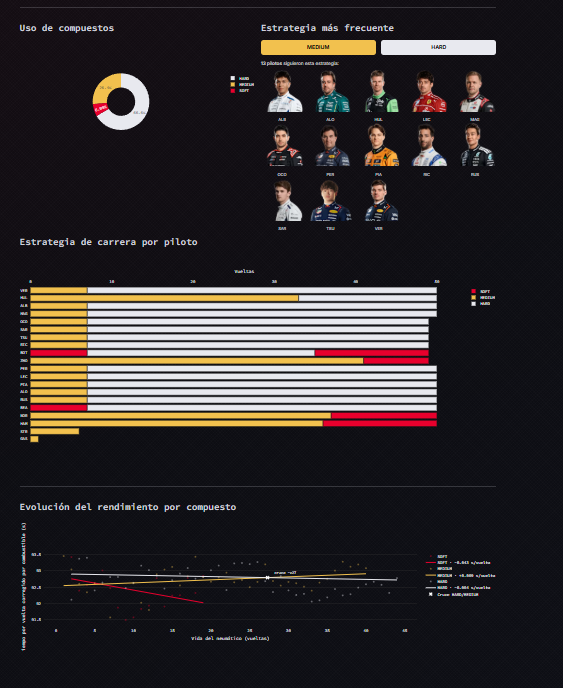
\includegraphics[width=0.72\textwidth]{neumaticos.png}
  \caption{Vista de Estrategia de Neumáticos: diagrama de Gantt de \textit{stints} por piloto, reparto de compuestos y curva de degradación.}
  \label{fig:neumaticos}
\end{figure}

\section{Análisis de piloto}
Si la categoría anterior ofrecía la vista de conjunto de un fin de semana, esta hace justo lo contrario ampliando el foco sobre un único piloto y vuelta para diseccionar cómo condujo. Todos los módulos de esta categoría parten de la telemetría de una vuelta de referencia, normalmente, la más rápida del piloto obtenida con el patrón de acceso descrito en la sección \ref{sec:datos}.
Estos datos se presentan de tres formas complementarias: como cifras de rendimiento, pintadas sobre el trazado del circuito, y como curvas de los distintos canales de telemetría. La categoría agrupa cuatro módulos desde un resumen del piloto hasta las trazas de telemetría.

\subsection{Resumen del Piloto}
El módulo \texttt{DriverReport.py} condensa el rendimiento de un piloto en una ficha. A partir de su vuelta más rápida extrae indicadores como velocidad punta y tiempos por sector. La Fórmula 1 divide cada circuito en tres sectores cronometrados de forma independiente, de modo que comparar sector a sector revela en qué parte del trazado un piloto gana o pierde tiempo.
Estos tiempos se presentan con su diferencia a la mejor marca, como puede verse en la Figura~\ref{fig:resumenpiloto}.

\begin{figure}[H]
  \centering
  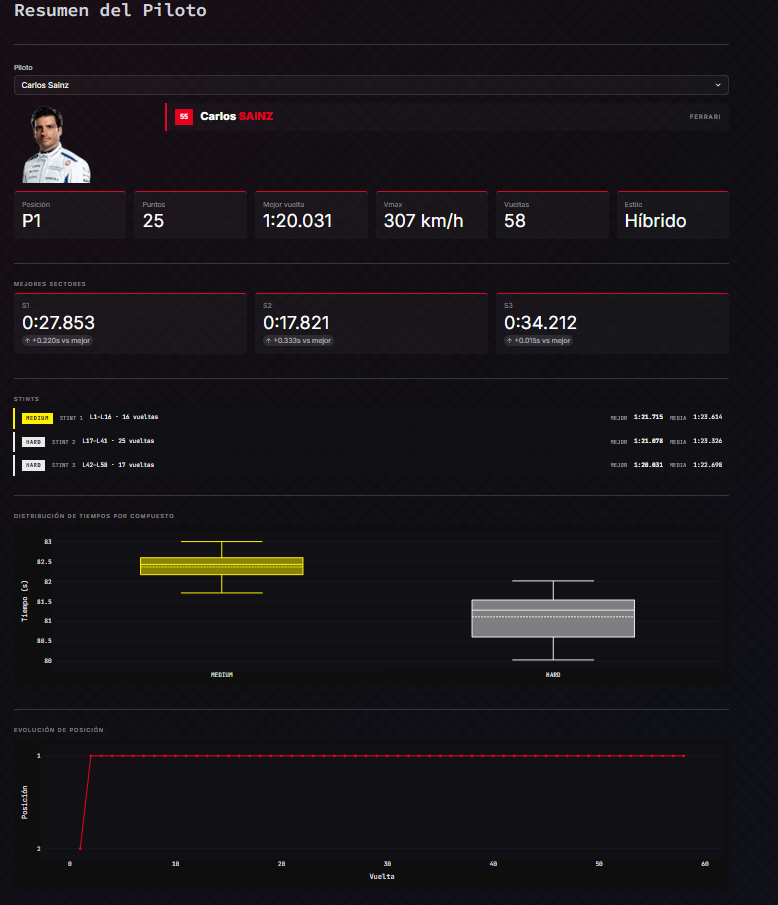
\includegraphics[width=0.72\textwidth]{resumenpiloto.png}
  \caption{Vista de Resumen del Piloto: KPIs de la vuelta, tiempos por sector y distribución de la sesión.}
  \label{fig:resumenpiloto}
\end{figure}

\subsection{Mapas sobre el trazado: velocidad y marchas}
Los módulos \texttt{SpeedHeatMap.py} y \texttt{GearHeatMap.py} comparten una misma idea y se explican juntos por ello. Tratan de proyectar un canal de telemetría sobre la silueta del circuito. Como cada muestra de telemetría incluye la posición del coche \texttt{X} e \texttt{Y} como su estado en ese instante, se puede dibujar el trazado y colorear cada punto según el valor que tomaba allí una variable completa.
Este estilo de dibujar la silueta del trazado está realizado de la misma forma que en el módulo \texttt{SessionSummary.py}, la documentación de FastF1 da una indicación sobre cómo dibujar el circuito.

\noindent En el \textbf{mapa de velocidad}, el color codifica la velocidad (canal \texttt{Speed}). De un solo vistazo se distinguen las rectas, donde el coche alcanza su máximo, de las curvas lentas, donde frena. En el \textbf{mapa de marchas}, el color muestra qué marcha usó el piloto en cada punto del trazado. Ambos permiten, opcionalmente, marcar las curvas numeradas para situarse mejor.

\noindent De forma común a ambos, la descarga de telemetría se separa del dibujado en una función cacheada con \texttt{@st.cache\_data}, porque este decorador no puede envolver código que contenga llamadas a la interfaz de Streamlit. Así, cambiar una opción de visualización no obliga a volver a descargar los datos. La Figura~\ref{fig:mapacalor} muestra un ejemplo de mapa de velocidad sobre el trazado.

\begin{figure}[H]
  \centering
  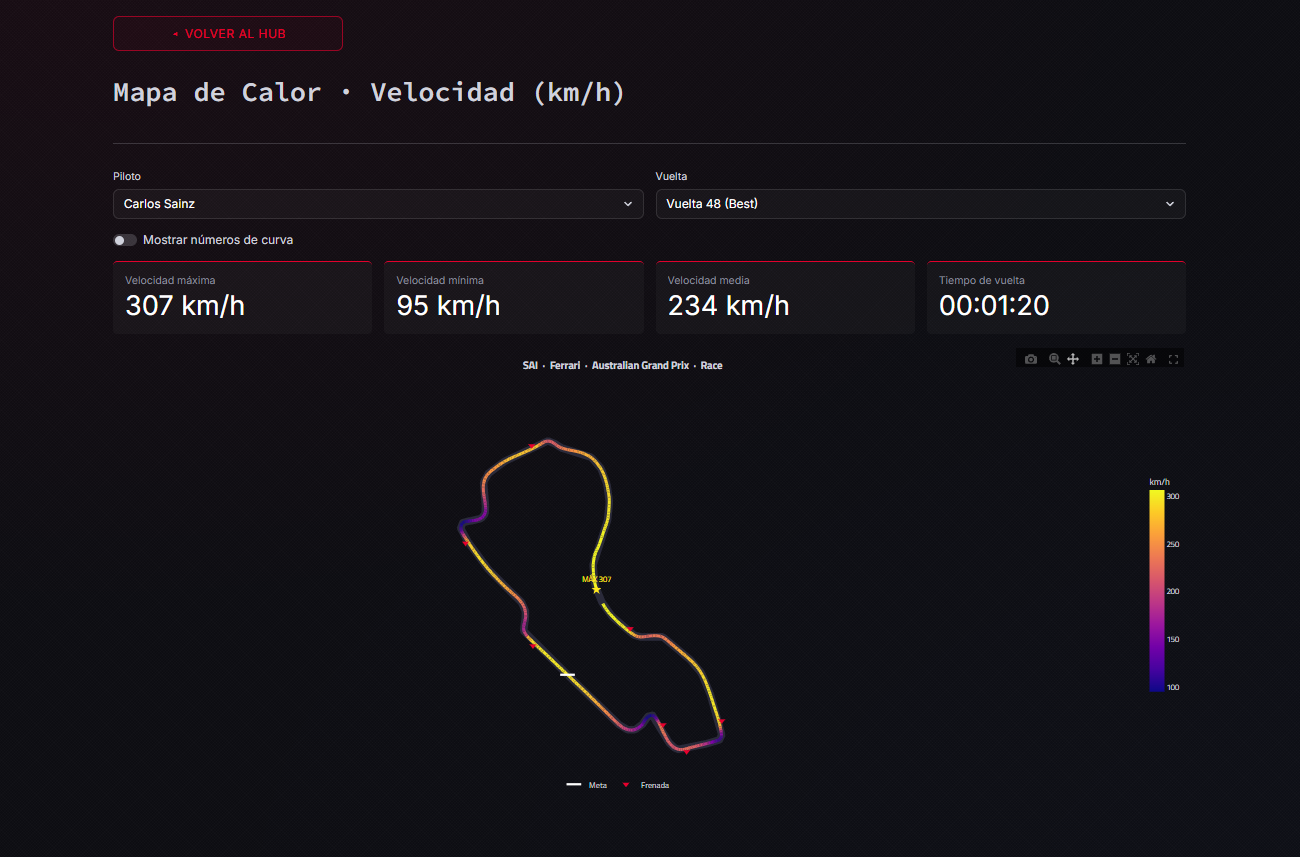
\includegraphics[width=0.72\textwidth]{mapacalor.png}
  \caption{Mapa de velocidad: el trazado del circuito coloreado según la velocidad en cada punto. El mapa de marchas es análogo, codificando la marcha seleccionada.}
  \label{fig:mapacalor}
\end{figure}

\subsection{Telemetry Trace}
El módulo \texttt{Telemetrytrace.py} es el más completo de la categoría y el que da acceso al detalle más fino. En lugar de proyectar un único canal sobre el circuito, representa la evolución de todos los canales de telemetría a lo largo de la vuelta: velocidad, acelerador, freno, marcha, revoluciones del motor \texttt{RPM} y \textit{DRS}, todos ellos frente a la distancia recorrida. Esto permite estudiar el estilo de conducción punto por punto,
dónde levanta el pie, cuánto tiempo frena, cuándo abre el DRS.

\noindent El \textit{DRS} (\textit{Drag Reduction System}) es un alerón trasero móvil que el piloto puede abrir para reducir la resistencia aerodinámica y ganar velocidad punta en las rectas. No se puede usar libremente, solo en zonas designadas del circuito y únicamente cuando se circula a menos de un segundo del coche de delante, ya que su finalidad es facilitar los adelantamientos. En la telemetría, el canal \texttt{DRS} indica si el sistema está abierto (Su valor es mayor a ocho) o cerrado en cada punto (menor o igual que ocho). La Figura~\ref{fig:drs} ilustra el efecto del DRS sobre el flujo de aire, con el alerón cerrado el flujo se desordena tras el ala generando resistencia, mientras que con el DRS abierto atraviesa la ranura de forma más limpia, reduciendo el \textit{drag}.

\begin{figure}[H]
  \centering
  \begin{subfigure}{0.49\textwidth}
    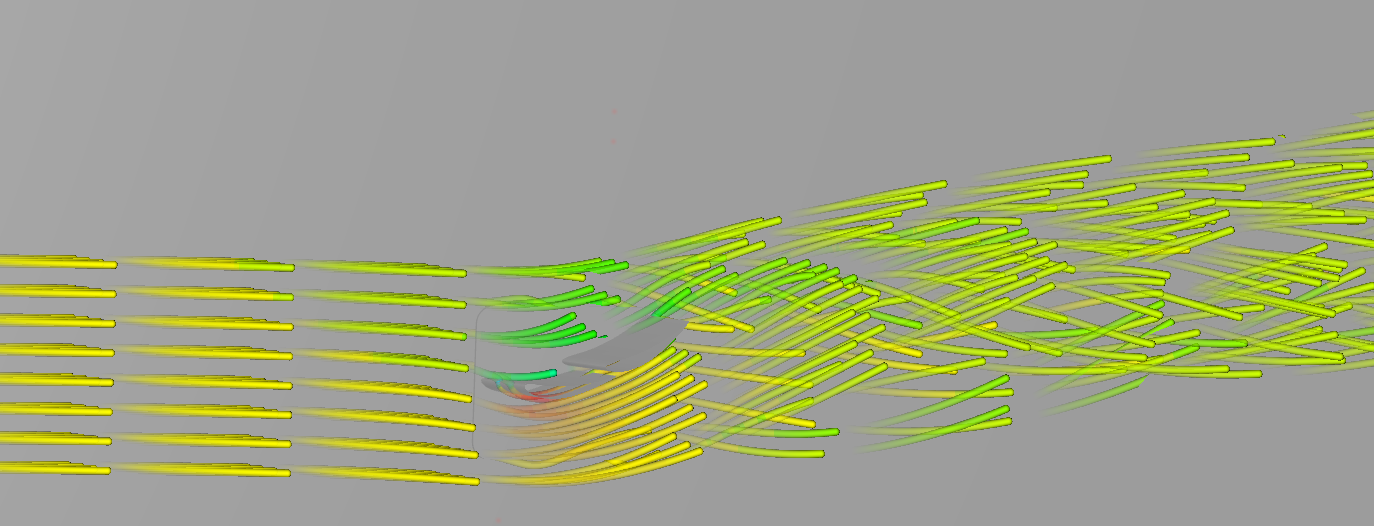
\includegraphics[width=\textwidth]{aleroncerrado.png}
    \caption{DRS cerrado}
  \end{subfigure}\hfill
  \begin{subfigure}{0.49\textwidth}
    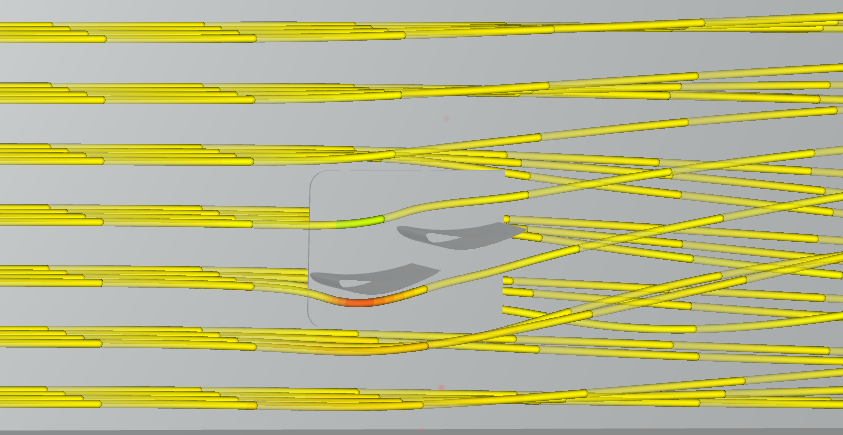
\includegraphics[width=\textwidth]{aleronabierto.png}
    \caption{DRS abierto}
  \end{subfigure}
  \caption[Efecto del DRS sobre el flujo de aire]{Simulación CFD ilustrativa del flujo de aire sobre el alerón trasero con el DRS cerrado y abierto. Imágenes propias realizadas sobre un modelo público de SimScale (autor: johmyang060323). Se incluye únicamente para ilustrar el concepto; no forma parte del desarrollo ni se emplean sus resultados cuantitativos.}
  \label{fig:drs}
\end{figure}

\noindent Conviene además mencionar que el canal de freno \texttt{Brake} se entrega en FastF1 como \textbf{binario}, indica únicamente si el piloto está frenando o no sin registrar la presión real sobre el pedal. Por ello lo que la herramienta representa como freno es un estado de apagado o encendido. La Figura~\ref{fig:telemetria} recoge esta vista con todos los canales.

\begin{figure}[H]
  \centering
  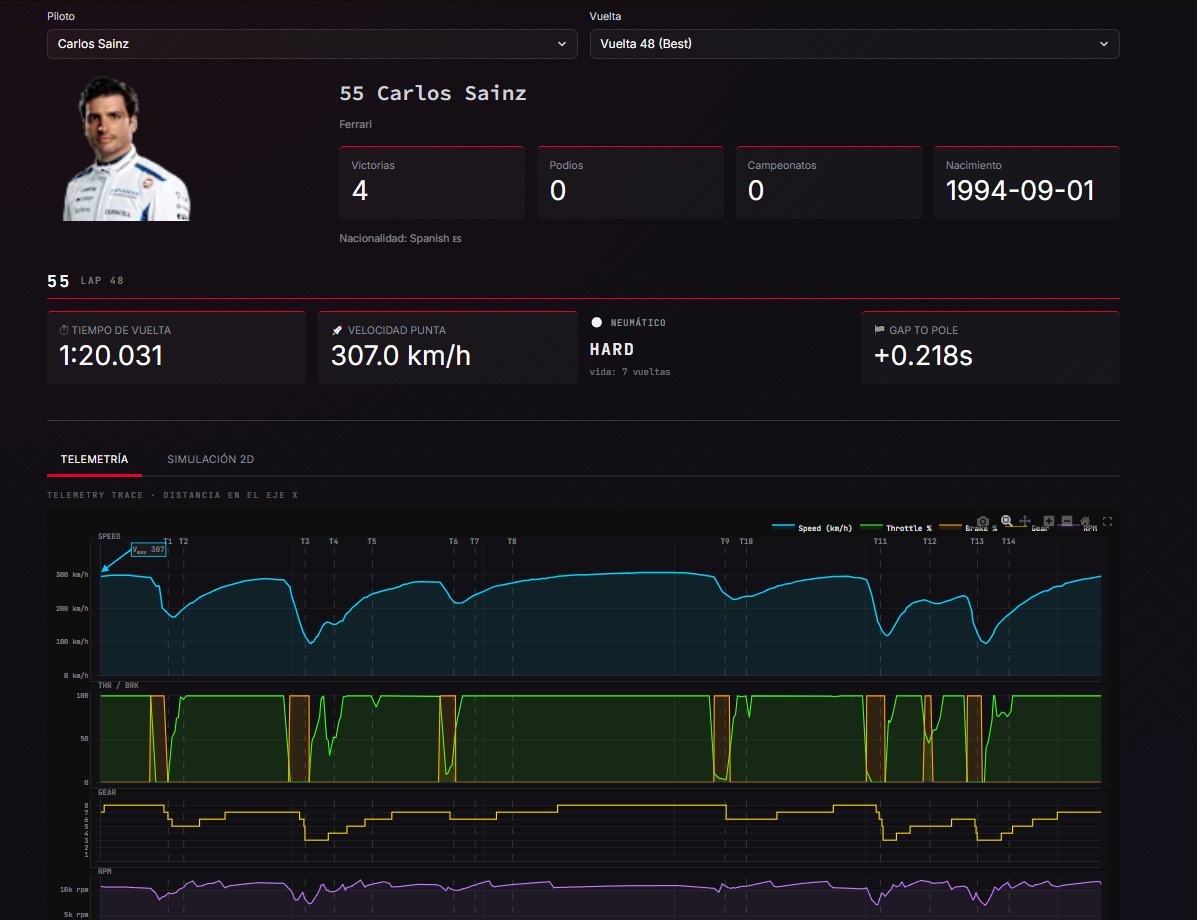
\includegraphics[width=0.72\textwidth]{telemetria.png}
  \caption{Vista de Telemetry Trace: evolución de los canales de telemetría (velocidad, acelerador, freno, marcha, RPM y DRS) a lo largo de la vuelta frente a la distancia.}
  \label{fig:telemetria}
\end{figure}

\noindent Este módulo es también el que integra los dos clasificadores de piloto: el \textit{tipo de vuelta} y la \textit{firma de pilotaje}. Ambos modelos construidos y validados en la sección \ref{sec:clasificadores}. La Figura~\ref{fig:ricciardostats} muestra ambos clasificadores en funcionamiento.

\begin{figure}[H]
  \centering
  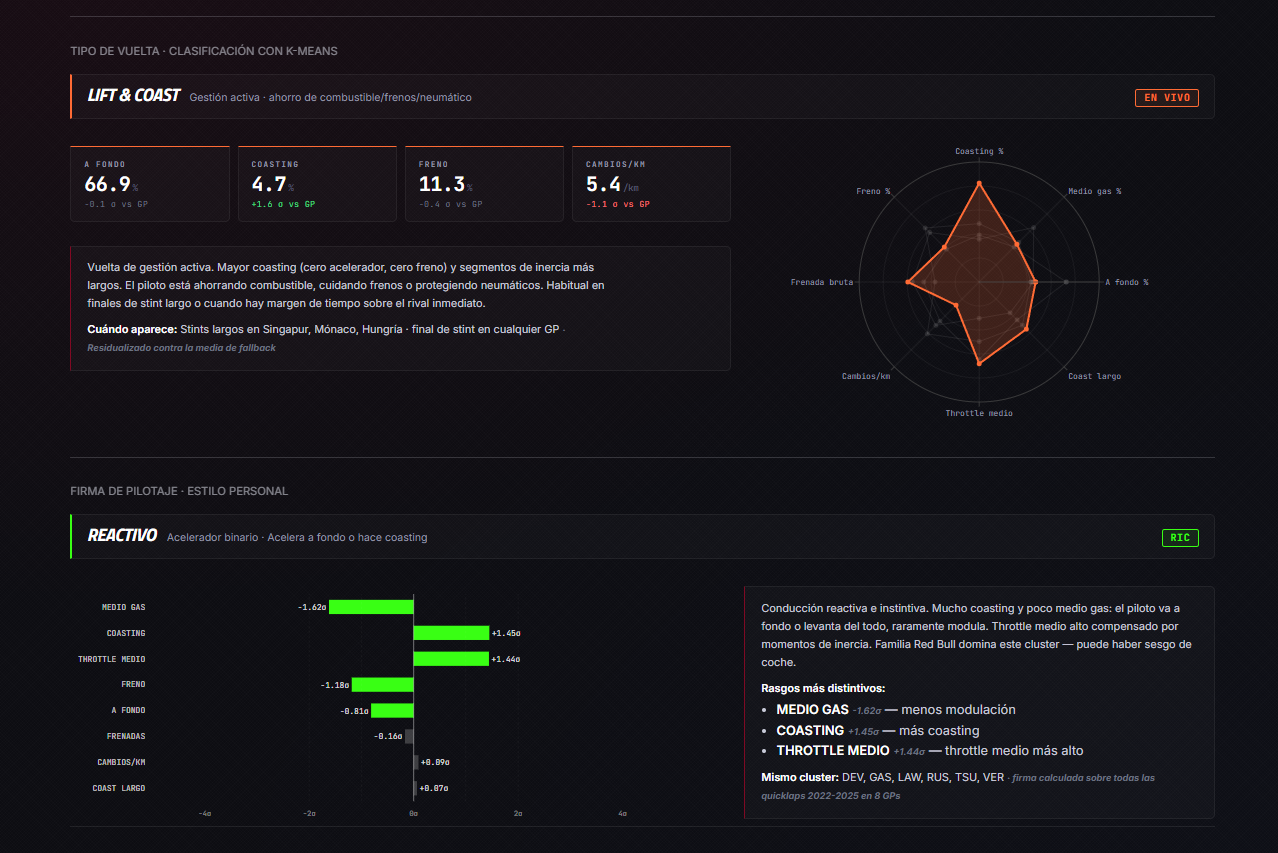
\includegraphics[width=0.72\textwidth]{ricciardostats.png}
  \caption{Los dos clasificadores en acción sobre una vuelta de Daniel Ricciardo (GP de Australia 2024): arriba el tipo de vuelta (\textit{Lift \& Coast}, gestión) y abajo la firma de pilotaje (\textit{Reactivo}), ambos calculados en vivo. Su construcción se detalla en la Sección~\ref{sec:clasificadores}.}
  \label{fig:ricciardostats}
\end{figure}

\subsubsection{Circuito animado}
Integrada dentro de la traza de telemetría, la herramienta ofrece una simulación animada de la vuelta. \texttt{Circuit2d.py}: un punto recorre el trazado a la vez que se desplazan unos paneles con la evolución de los pedales, marcando además las zonas de DRS y los tiempos por sector con el código de colores habitual de la retransmisión (morado para el mejor tiempo absoluto, verde para el mejor personal, amarillo para el resto).

\noindent Este módulo es un ejemplo de decisión motivada por el rendimiento. En su primera iteración la animación se generaba con \textit{Matplotlib}, renderizándola como vídeo que se descargaba e incrustaba como HTML en la página. El enfoque funcionaba, pero era costoso de generar y lento de cargar. Se reimplementó por completo de forma nativa en \textit{Plotly}, como una animación interactiva sin paso intermedio por vídeo, eliminando así la descarga y reduciendo el tiempo de carga. La Figura~\ref{fig:circuit2d} muestra un fotograma de esta simulación.

\begin{figure}[H]
  \centering
  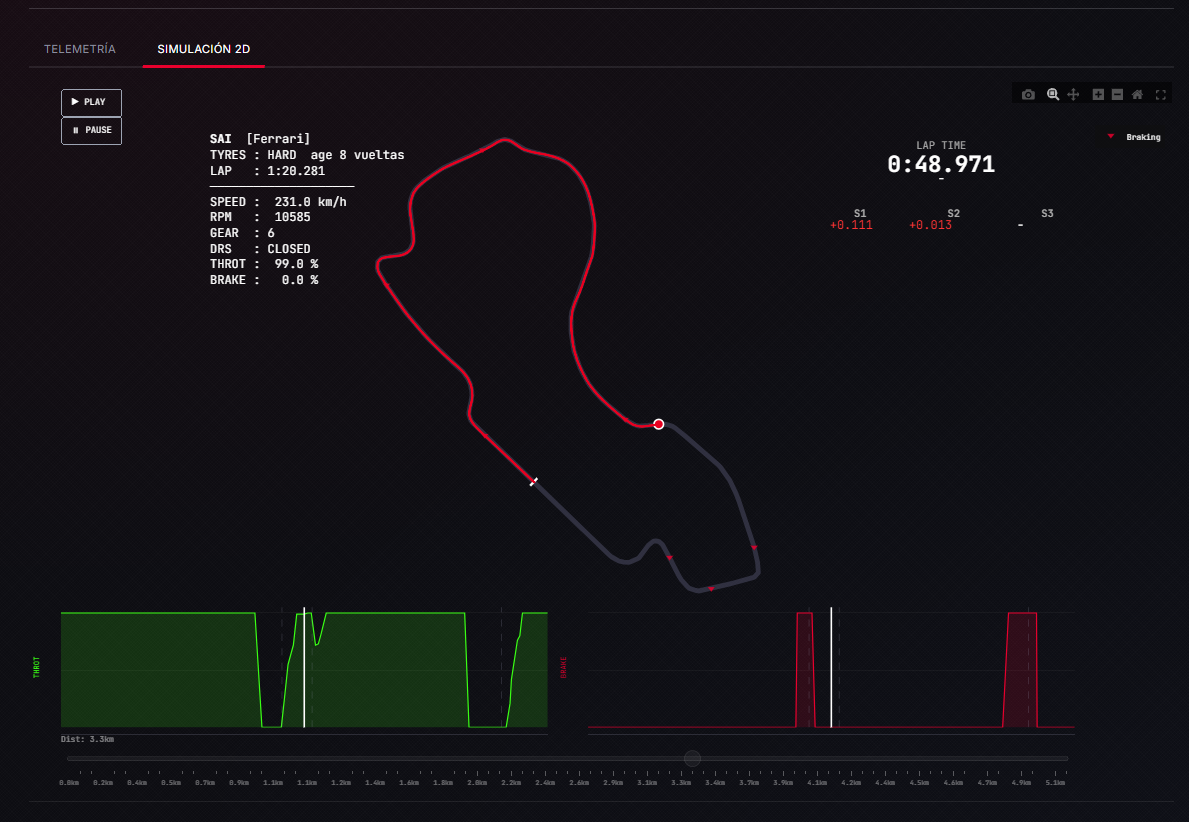
\includegraphics[width=0.72\textwidth]{circuit2d.png}
  \caption{Simulación animada de la vuelta: un punto recorre el trazado mientras se desplazan los paneles de pedales y se marcan zonas de DRS y tiempos por sector.}
  \label{fig:circuit2d}
\end{figure}

\section{Análisis comparativo}
Las dos primeras categorías analizan a un piloto o un evento de forma aislada. Esta tercera se dedica a enfrentar a dos o más pilotos entre sí, que es donde el análisis de telemetría revela quién es más rápido y, sobre todo, dónde. Toda la categoría comparte un reto técnico común.

\noindent La telemetría de dos vueltas no es directamente comparable: cada una contiene sus muestras en puntos distintos del trazado, porque dependen del tiempo y no de la posición. Superponerlas en crudo no tiene sentido. La solución, común a todos los módulos de esta categoría, es interpolar ambas vueltas sobre una rejilla de distancia común. Se define una malla de puntos
igualmente espaciados a lo largo del trazado y se muestrea cada canal de cada vuelta sobre esa malla. Una vez ambas vueltas comparten el mismo eje distancia, sus puntos corresponden uno a uno y la comparación es legítima. Sobre esa base se calcula el \textit{delta}: la diferencia de tiempo acumulada entre las dos vueltas en cada punto del circuito, que indica cuánto tiempo gana o pierde un piloto respecto al otro a lo largo de la vuelta.
El listado \ref{lst:interp} muestra cómo se interpolan dichos canales.
\begin{lstlisting}[style=python,caption={Interpolación de una vuelta sobre la rejilla común en \texttt{Ghostcar.py}.},label=lst:interp]
def _interpolate_on_grid(tel, dist_grid, ref_dist_max):
    src_dist = tel["Distance"].values.astype(float)
    # Normalizar por fracción de vuelta (robusto a trazadas de distinta longitud)
    frac_orig = src_dist / src_dist[-1]
    frac_grid = dist_grid / ref_dist_max

    # Remuestrear cada canal sobre la rejilla común
    speed  = np.interp(frac_grid, frac_orig, tel["Speed"].values)

    # Tiempo acumulado (clave para el delta), forzado a empezar en 0
    time_s = tel["Time"].dt.total_seconds().values
    time_s = np.interp(frac_grid, frac_orig, time_s - time_s[0])
    # ... (resto de canales: throttle, brake, gear, rpm, drs)
    return {"speed": speed, "time_s": time_s, ...}
\end{lstlisting}

\subsection{Panel de Equipo}
El módulo \texttt{TeamTelemetry.py} enfrenta a los dos pilotos de un mismo equipo. Estos dos pilotos comparten monoplaza y son por tanto la comparación más limpia posible. Se muestra su telemetría de forma simétrica con una vista inspirada en las interfaces de telemetría que los propios equipos usan en el muro de boxes durante la retransmisión.
Se añade en el centro el circuito dibujado indicando en una misma vuelta donde se encontraban físicamente dichos pilotos.

\subsection{Comparativa de sesión}
El módulo \texttt{OverallStandings.py} superpone los canales de telemetría de varios pilotos sobre una misma vuelta, se interpolan sobre la rejilla común permitiendo de esta manera contrastar los mismos canales de telemetría que encontrábamos en \texttt{Telemetrytrace.py}. La herramienta permite seleccionar hasta cuatro pilotos para superponer su telemetría.
Este módulo cuenta también con una sección \textit{Head 2 Head} que permite ver el dominio de un piloto sobre otro de forma visual viéndolo sobre el circuito pintado. También nos permite mirar el delta acumulado de las dos vueltas seleccionadas.

\noindent Por último permite ver un desglose de los \textit{stints} de los pilotos seleccionados viendo la evolución del compuesto por vuelta y una tabla resumen de los \textit{stints}.

\subsection{La vuelta ideal}
El módulo de \texttt{OptimalLap.py} construye una vuelta teórica perfecta, que ningún piloto llega a dar. Una vuelta teórica se construye dividiendo el circuito en un número a seleccionar de \textit{microsectores} (Pequeños tramos consecutivos). Para cada microsector identifica qué piloto y equipo fue el más rápido en él. La vuelta ideal es el mosaico resultante con cada pequeño sector coloreado con el equipo dominante y su tiempo es la suma de los mejores tiempos
parciales de toda la parrilla. Representa el límite absoluto de rendimiento alcanzable en ese circuito combinando lo mejor de cada coche.
El módulo permite filtrar por equipo para solo ver los resultados de determinadas escuderías. La Figura~\ref{fig:vueltaideal} muestra esta vuelta ideal por microsectores.


\begin{figure}[H]
  \centering
  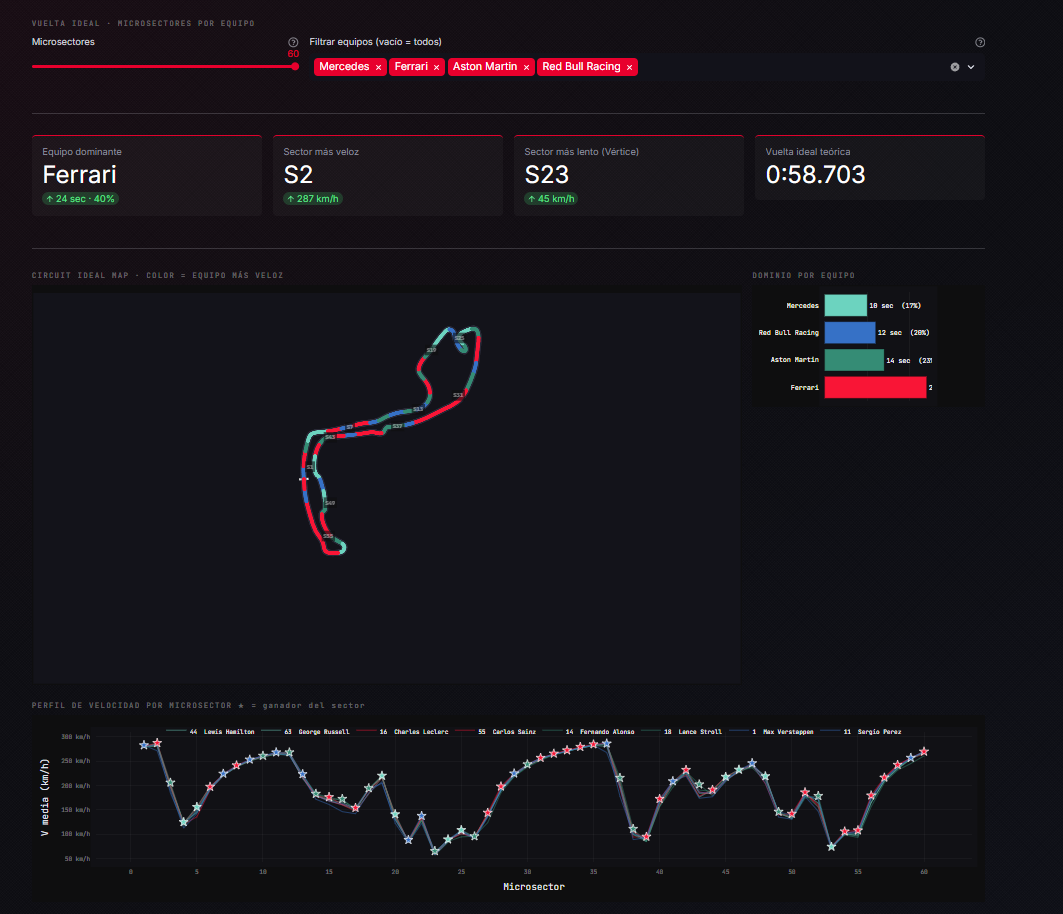
\includegraphics[width=0.72\textwidth]{vueltaideal.png}
  \caption{La Vuelta Ideal: el circuito dividido en microsectores, cada uno coloreado con el equipo más rápido en él y filtrado por equipos. El tiempo resultante es la suma de los mejores parciales de toda la parrilla.}
  \label{fig:vueltaideal}
\end{figure}

\subsection{Coche fantasma}
El módulo \texttt{Ghostcar.py} lleva la comparación al plano visual. Tras interpolar dos vueltas sobre la rejilla común, las reproduce como una \textbf{animación de persecución} donde dos coches recorren el trazado simultáneamente y, al ir cada uno a su ritmo real, el más rápido se distancia progresivamente del otro. El nombre alude a la mecánica del \textit{coche fantasma} de los videojuegos de conducción. La animación se acompaña del gráfico de \textit{delta}, de modo que la diferencia de tiempo no solo se ve crecer entre los coches sino que se cuantifica en cada punto de la vuelta. La Figura~\ref{fig:fantasma} recoge un ejemplo de esta comparación.

\begin{figure}[H]
  \centering
  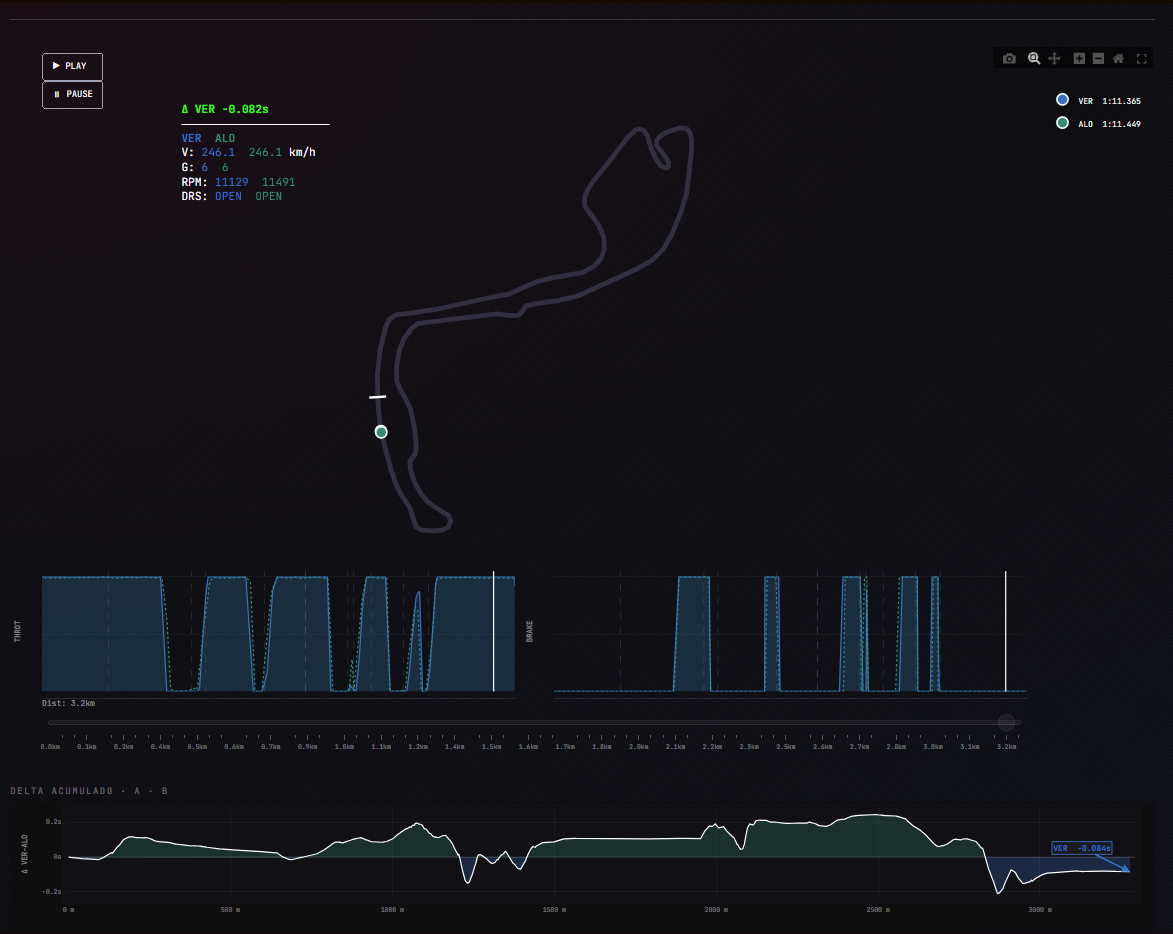
\includegraphics[width=0.72\textwidth]{monaco23.png}
  \caption{Coche Fantasma (Qualy GP de Mónaco 2023): dos vueltas interpoladas sobre la rejilla común se reproducen como persecución; abajo, la curva del delta acumulado entre ambas.}
  \label{fig:fantasma}
\end{figure}

\section{Dinámica vehicular}
La última de las cuatro categorías es la más física de todas. Mientras las anteriores presentan o comparan canales de telemetría, esta los transforma en magnitudes físicas que no vienen medidas en los datos. Las fuerzas que actúan sobre el monoplaza son el núcleo del que parten los tres módulos de esta categoría.

\subsection{Fundamento físico}
Una fuerza G es una forma intuitiva de expresar una aceleración. Es el número de veces que esta fuerza supera a la aceleración de la gravedad ($g = 9{,}81$~m/s$^2$). Cuando se dice que un piloto soporta 5G en una frenada, significa que su cuerpo experimenta una fuerza equivalente a cinco veces su peso. Es la magnitud que mejor comunica lo extremo del entorno físico de la Fórmula 1.

\noindent Sobre el coche actúan dos componentes independientes. La \textbf{aceleración longitudinal} actúa en la dirección del movimiento, es positiva al acelerar y negativa al frenar. La \textbf{aceleración lateral} actúa perpendicular a la marcha y aparece en las curvas, empujando el coche hacia el exterior del giro.

\noindent Las limitaciones técnicas son claras puesto que FastF1 no entrega aceleraciones. Entrega la posición del coche y su velocidad escalar. Las fuerzas G hay que \textbf{derivarlas} de esos datos.

\paragraph{Aceleración longitudinal.} Es la más directa. La aceleración es, por definición, la variación de la velocidad con el tiempo:
\begin{equation}
a_{\text{lon}} = \frac{dv}{dt}, \qquad G_{\text{lon}} = \frac{a_{\text{lon}}}{g}.
\end{equation}
\noindent Como la velocidad $v$ está disponible, basta con derivarla respecto al tiempo.

\paragraph{Aceleración lateral.} Es más sutil, porque no puede obtenerse de la velocidad escalar. Un coche puede ir a velocidad constante y aun así sufrir una gran aceleración lateral si gira. Aquí entra la física del movimiento circular. 
Un coche que toma una curva de radio $R$ describe un arco, y para no salirse en línea recta necesita una \textbf{aceleración centrípeta} dirigida hacia el centro de la curva:
\begin{equation}
a_{\text{lat}} = \frac{v^2}{R} = v \cdot \omega,
\end{equation}
donde $\omega = v/R$ es la \textbf{velocidad angular} o ritmo de giro: cuántos radianes por segundo cambia la dirección de marcha del coche. Esta dirección, el \textit{heading} $\theta$, se obtiene de cómo varía la posición:
\begin{equation}
\theta = \arctan\!2\!\left(\frac{dY}{dt}, \frac{dX}{dt}\right), \qquad \omega = \frac{d\theta}{dt}.
\end{equation}
Es decir, se mira hacia dónde apunta la trayectoria en cada instante y se calcula la rapidez con la que ese ángulo cambia. Multiplicando por la velocidad se obtiene la aceleración lateral.

\paragraph{Uso de la teoría}
Las fórmulas son exactas, pero aplicarlas sobre datos GPS muestreados tiene un problema. Al derivar dos veces la posición se \textbf{amplifica el ruido}. Por ello el cálculo añade tres protecciones mínimas, sin alterar la física. Se añade un filtro de tipo Savitzky-Golay (toda derivada numérica de datos discretos lo requiere), la anulación de la G lateral por debajo de 30 km/h donde la dirección de marcha no es fiable, como en el \textit{pit lane} o las vueltas de entrada y salida y un recorte final al límite físico de $\pm 6$G como red de seguridad. El listado siguiente recoge el cálculo completo.

\paragraph{Savitzky-Golay} Derivar numéricamente una señal muestreada amplifica el ruido de alta frecuencia, por lo que antes de derivar se suaviza con un filtro Savitzky-Golay~\cite{savgol1964,savitzky_schafer2011}. A diferencia de una media móvil que aplana los picos, este filtro ajusta por mínimos cuadrados un polinomio de grado bajo a una ventana deslizante $2m+1$ muestras y evalúa ese polinomio en el punto central.
\begin{equation}
y_i^{\text{suav}} = \sum_{j=-m}^{m} c_j \, y_{i+j},
\end{equation}
donde los coeficientes $c_j$ se obtienen del ajuste polinómico y solo dependen del tamaño de la ventana y el grado del polinomio. De este modo se reduce el ruido preservando la forma de los picos de aceleración, que es justo lo que interesa conservar. La implementación emplea la función \texttt{savgol\_filter} de SciPy con una ventana equivalente a medio segundo y un polinomio de grado tres.
Podemos observar en el listado \ref{lst:gforces} como se calculan las fuerzas y cómo se usa el filtro mencionado.
\begin{lstlisting}[language=Python,caption={Cálculo de las fuerzas G en \texttt{GGDiagram.py}.},label=lst:gforces]
# G longitudinal: derivada de la velocidad
g_lon = savgol_filter(np.gradient(speed_ms, time_s) / 9.81, win, poly)

# G lateral: v * omega, con omega = ritmo de giro de la dirección
x = savgol_filter(tel["X"].values, win, poly)
y = savgol_filter(tel["Y"].values, win, poly)
heading = np.unwrap(np.arctan2(np.gradient(y, time_s),
                               np.gradient(x, time_s)))
omega = np.gradient(heading, time_s)
g_lat = savgol_filter(speed_ms * omega / 9.81, win, poly)
g_lat[speed_ms < 30/3.6] = 0.0   # dirección no fiable a baja velocidad

g_total = np.sqrt(g_lat**2 + g_lon**2)
\end{lstlisting}

\paragraph{Validación del método}
El cálculo longitudinal es sólido, aplicado a vueltas de clasificación produce frenadas pico del orden de 5G que está en línea con las cifras públicas de la categoría. El cálculo lateral, en cambio, es una \textbf{estimación cinemática a partir del GPS}, no una medida de una unidad inercial real. La estimación de la dinámica de un vehículo de competición a partir de sensores de posición y velocidad es un problema estudiado en la literatura~\cite{wischnewski2019}. Captura fielmente la forma de las cargas en curva, pero el ruido de la señal de posición tiende a sobreestimar los picos, que se acotan al límite físico. Se documenta así siendo un estimador, no una medición instrumentada.

\subsection{El Diagrama G-G}
El módulo \texttt{GGDiagram.py} representa cada instante de la vuelta como un punto en un plano cuyos ejes son la G lateral y la G longitudinal. El resultado es el llamado \textbf{círculo de tracción} o círculo de fricción, un concepto clásico de la dinámica del neumático~\cite{pacejka2012}. La idea física es que un neumático dispone de un cierto límite de agarre al que el piloto puede aproximarse frenando, girando o una combinación de ambos, pero cuya suma no puede superar cierto máximo o el coche se descontrolará. La envolvente convexa de todos los puntos dibuja ese límite, y su forma revela el estilo de pilotaje: un buen piloto mantiene los puntos pegados al borde, exprimiendo el agarre disponible en todo momento.


\subsection{Carga Aerodinámica}
La aerodinámica es uno de los pilares del rendimiento en Fórmula 1~\cite{katz2006}. Al avanzar, el coche genera \textbf{carga aerodinámica} (\textit{downforce}). Una fuerza vertical que lo presiona contra el asfalto y aumenta el agarre, a costa de una resistencia al avance (\textit{drag}). Ambas fuerzas comparten la misma forma física y crecen con el \textbf{cuadrado de la velocidad}, diferenciándose únicamente en el coeficiente aerodinámico:
\begin{equation}
L = \tfrac{1}{2}\,\rho\,v^2\,C_l\,A, \qquad D = \tfrac{1}{2}\,\rho\,v^2\,C_d\,A,
\end{equation}
donde $L$ es la carga aerodinámica (\textit{downforce}) y $D$ la resistencia (\textit{drag}); $\rho$ es la densidad del aire, $v$ la velocidad, $A$ el área frontal y $C_l$, $C_d$ los coeficientes de sustentación y resistencia respectivamente. Esta dependencia con $v^2$ es la clave que permite detectar la carga aerodinámica a partir de la telemetría.

\medskip
\noindent El razonamiento del módulo \texttt{Aero.py} es el siguiente. Sin aerodinámica, el agarre lateral máximo de un coche sería constante, fijado solo por el agarre mecánico (basado en neumáticos y peso). Pero con \textit{downforce}, ese agarre crece con la velocidad, porque la carga vertical aumenta con la velocidad al cuadrado. El máximo agarre lateral se modela entonces como:
\begin{equation}
G_{\text{lat,max}}(v) = \alpha + \beta \, v^2,
\end{equation}
donde $\alpha$ representa el agarre mecánico base y $\beta$ la ganancia por carga aerodinámica. Si al ajustar este modelo resulta que $\beta > 0$
con significación estadística, se tiene evidencia de la firma del \textit{downforce}. El módulo agrupa los datos por velocidad, calcula la envolvente de agarre lateral en cada tramo y realiza una regresión por mínimos cuadrados de la envolvente frente a $v^2$, reportando la pendiente $\beta$, el coeficiente de determinación $R^2$ y el $p$-valor.

\noindent En cuanto al alcance del módulo, este \textbf{detecta la firma} de la carga aerodinámica de forma relativa, no la mide en Newtons. Los parámetros $\alpha$ y $\beta$ son compuestos puesto que no separan masa, área ni coeficientes y solo son interpretables comparativamente entre pilotos y sesiones. Es una estimación indirecta a partir de la telemetría, sin instrumentación física. La simulación de la Figura~\ref{fig:cfd} se incluye para ilustrar el concepto.

\begin{figure}[H]
  \centering
  \begin{subfigure}{0.48\textwidth}
    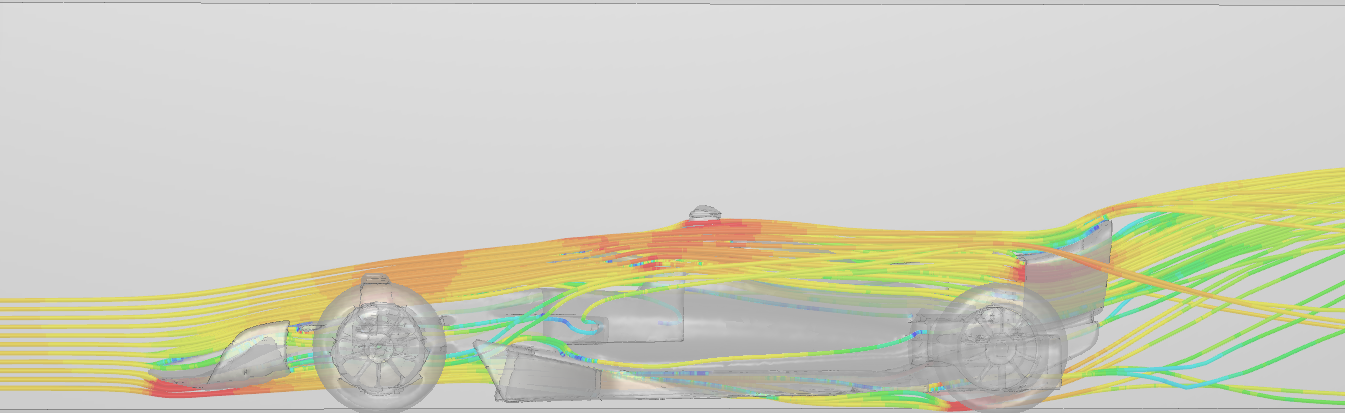
\includegraphics[width=\textwidth]{sideview.png}
    \caption{Vista lateral}
  \end{subfigure}\hfill
  \begin{subfigure}{0.48\textwidth}
    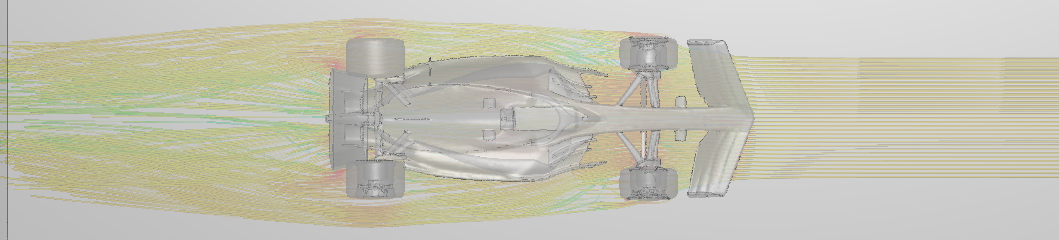
\includegraphics[width=\textwidth]{topview.png}
    \caption{Vista superior}
  \end{subfigure}

  \vspace{0.6em}
  \begin{subfigure}{0.48\textwidth}
    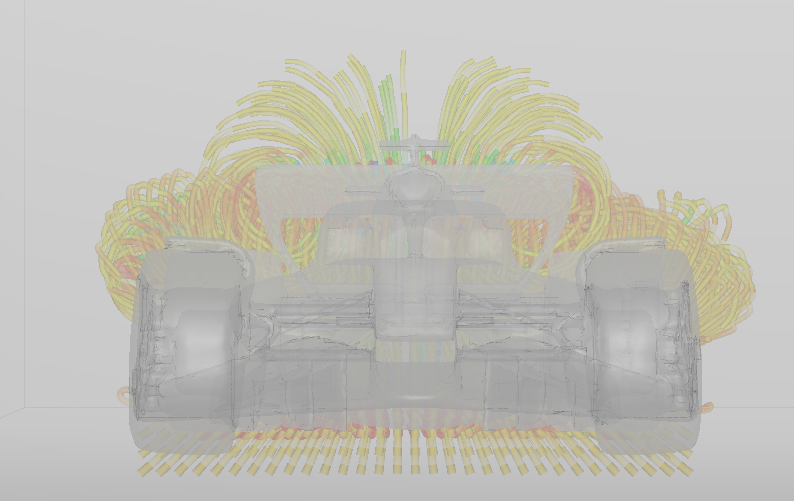
\includegraphics[width=\textwidth]{front.png}
    \caption{Vista frontal}
  \end{subfigure}\hfill
  \begin{subfigure}{0.48\textwidth}
    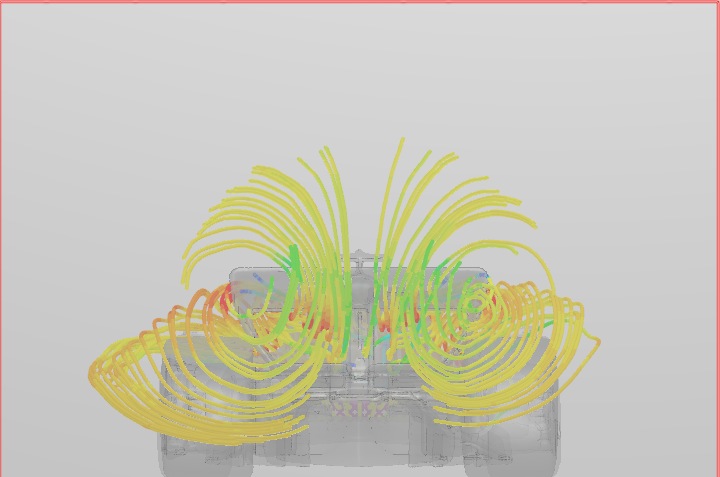
\includegraphics[width=\textwidth]{rearview.png}
    \caption{Vista trasera}
  \end{subfigure}
  \caption[Visualización CFD ilustrativa del flujo aerodinámico]{Simulación CFD ilustrativa del flujo de aire alrededor de un monoplaza, coloreada por magnitud de velocidad. Se aprecian la estela tras el coche y los vórtices de borde, fenómenos centrales en la aerodinámica de un Fórmula 1~\cite{guerrero2020}. Imágenes propias realizadas sobre un modelo público en SimScale (autor del modelo: alex\_gugan). Se incluye únicamente para ilustrar el concepto de carga aerodinámica; no forma parte del desarrollo ni se emplean sus resultados cuantitativos.}
  \label{fig:cfd}
\end{figure}

\subsection{Carga por rueda}
El último módulo, \texttt{TyreLoad.py}, estima cómo se reparte la carga entre las cuatro ruedas a lo largo de la vuelta. La base física es la \textbf{transferencia de masas}. Cuando el coche frena, el peso se desplaza hacia el eje delantero, cuando toma una curva se desplaza hacia las ruedas exteriores. Estas transferencias son proporcionales a las fuerzas G calculadas anteriormente y a la geometría del coche, donde $h$ es la altura del centro de gravedad, $L$ la distancia entre ejes y $t$ el ancho de vía:
\begin{equation}
\Delta F_{z,\text{lon}} \propto G_{\text{lon}} \cdot \frac{h}{L}, \qquad
\Delta F_{z,\text{lat}} \propto G_{\text{lat}} \cdot \frac{h}{t}.
\end{equation}
A la carga estática se le suman estas transferencias y la carga aerodinámica. Dicha carga crece con la velocidad y se reduce al activar el DRS. Comparando la fuerza que cada neumático debe transmitir con la que es capaz de soportar se obtiene su \textit{exigencia}, una medida de cuánto se está estresando cada goma. La Figura~\ref{fig:tyreload} muestra esta representación de la carga por rueda.

El modelo es físicamente correcto en la formulación puesto que las leyes de transferencia de masas son las estándar de la dinámica vehicular~\cite{gillespie1992,milliken1995}, si bien los parámetros del vehículo son valores realistas asumidos y no medidos del coche concreto. Es, por tanto, una estimación coherente y físicamente fundamentada y no una medición exacta por falta de datos.
\begin{figure}[htbp]
  \centering
  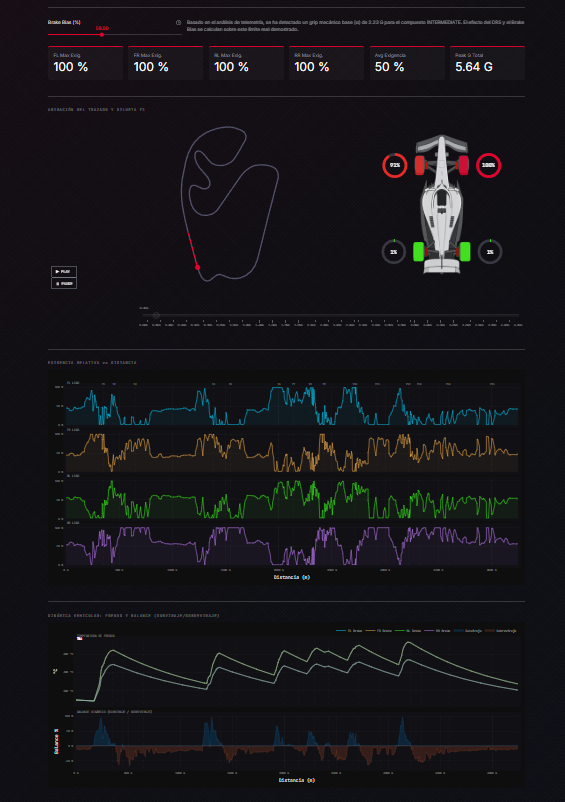
\includegraphics[width=0.78\textwidth]{TyreLoad.png}
  \caption{Mapa de Carga por Rueda: estimación de la carga vertical y la exigencia sobre cada neumático a lo largo de la vuelta, derivada de las transferencias de masa. Curva número 1 de brasil, frenada fuerte.}
  \label{fig:tyreload}
\end{figure}

\section{Modelos de aprendizaje no supervisado}\label{sec:clasificadores}
Tres de los módulos de la herramienta no se limitan a mostrar datos, sino que clasifican asignando una etiqueta interpretable a partir de la telemetría. Estos tres clasificadores comparten la misma arquitectura de aprendizaje automático, descrita de forma unificada en esta sección.

\subsection{El problema y el enfoque no supervisado}
El objetivo es agrupar miles de observaciones (vueltas, circuitos o pilotos) en familias de comportamiento similar, sin disponer de etiquetas previas. Nadie ha marcado de antemano qué vuelta es de \textit{ataque}, \textit{gestión} o qué circuito es \textit{urbano}. Este es un problema de \textbf{aprendizaje no supervisado}, en el que el algoritmo descubre la estructura de datos por sí mismo. La técnica empleada es \textbf{K-Means}, uno de los algoritmos más establecidos.

\subsection{Representación de las características}
Un algoritmo de agrupamiento no entiende de etiquetas como vueltas o circuitos, solo de números. Por ello, cada observación se resume en un \textit{vector de características}, una lista de valores numéricos que la describen.
Una vuelta, por ejemplo, se representa con ocho características de pilotaje (porcentaje de tiempo a pleno gas, frenada, inercia o \textit{coasting}, cambios de marcha por kilómetro, entre otras), mientras que un circuito se describe mediante sus fuerzas G. Cada observación se convierte así en un punto dentro de un espacio de tantas dimensiones como \textit{features} tenga.

\subsection{Cómo agrupa K-Means}
K-Means divide los puntos en $k$ grupos buscando minimizar la distancia de cada punto al centro del grupo. El proceso es iterativo. Se colocan $k$ centros iniciales, a cada punto se le asigna el más cercano. Cada centro se recoloca en la media de los puntos que se le han asignado y se repite hasta que los centros se estabilizan. El resultado por tanto serán $k$ \textbf{centroides}, cada uno representando el punto medio de una familia. Una observación nueva se clasifica calculando a qué centroide está más cerca.

\subsection{Refinamiento sobre el modelo base}
El enfoque básico se mejora con dos técnicas que resultaron decisivas para la calidad de la clasificación.

\paragraph{Residualización por circuito} En el clasificador de tipo de vuelta, comparar valores crudos sería engañoso. Una vuelta en Mónaco siempre tendrá poco tiempo a pleno gas por la naturaleza del circuito, no por el estilo del piloto o por el tipo de vuelta. Para aislar el comportamiento del piloto del efecto del trazado, a cada vuelta se le resta la media de su Gran Premio. De este modo las características no miden cuánto acelera el piloto, sino cuánto se desvía de lo normal en ese circuito, haciendo comparables vueltas de circuitos distintos.

\paragraph{Reducción de dimensionalidad con PCA} En el clasificador de estilo de pilotaje, las ocho características están muy correlacionadas entre sí. El porcentaje a pleno gas y la media del acelerador, por ejemplo, miden cosas parecidas. Esta redundancia dispersa los grupos y dificulta la separación. Para resolverlo se aplica \textbf{Análisis de Componentes Principales} (PCA), una técnica que reescribe los datos en un número menor de dimensiones, las que capturan la mayor variación, descartando la redundancia. Proyectando las ocho características sobre sus dos componentes principales, que conservan en torno al 65\% de la información, la separación entre grupos prácticamente se duplicó.

\paragraph{Entrenamiento offline e inferencia en vivo}
El cálculo de los centroides es costoso, pero solo necesita realizarse una vez. Por ello el entrenamiento se ejecuta de forma aislada en los \textit{scripts} en la carpeta reservada a investigación, apoyados en la implementación de K-Means y PCA de scikit-learn. Los centroides resultantes se almacenan como constantes en los módulos de producción. En tiempo de ejecución la aplicación no reentrena nada. Simplemente extrae las características de la observación, las compara con los centroides ya calculados y devuelve la etiqueta más próxima de forma instantánea.
El preprocesado previo al entrenamiento difiere según el clasificador. El de tipo de vuelta, que opera sobre vueltas individuales, depura el conjunto con un \textit{Isolation Forest} que aísla y descarta en torno al 5\% de observaciones anómalas (vueltas tras coche de seguridad, de entrada y salida de boxes o con telemetría corrupta) antes de calcular los centroides. Los clasificadores de pilotaje y circuito no lo requieren, ya que trabajan sobre datos agregados (la media de las vueltas de cada piloto o de cada circuito), y esa agregación diluye por sí misma el efecto de las observaciones atípicas.
\paragraph{Observaciones atípicas}
Si una observación queda demasiado lejos de todos los centroides, más allá de un umbral, no se le fuerza una etiqueta, sino que se marca como \textit{atípica} o \textit{híbrido} en el caso de pilotos. Esto es deliberado, ya que es preferible admitir que un perfil no encaja limpiamente a inventar una clasificación falsa. La validación cuantitativa de los clasificadores se presentará en el capítulo \ref{cap:validacion}.

\chapter{Validación y Pruebas}\label{cap:validacion}
La validación de este trabajo se aborda en tres niveles complementarios, que cubren desde la corrección de cálculos internos hasta el comportamiento de cara al usuario. En primer lugar, una validación funcional comprueba que la herramienta reproduce hechos conocidos y verificables.
En segundo lugar, una batería de pruebas unitarias verifica de forma automática la corrección de las funciones de cálculo. Por último, los modelos de aprendizaje no supervisado se evalúan con métricas específicas. Esta estructura sigue la pirámide habitual de validación desde la unidad más pequeña a la aceptación del sistema como conjunto.

\section{Validación funcional}
El objetivo de esta primera validación es comprobar que la información que presenta la herramienta se corresponde con la realidad de cada sesión. Para ello no basta con inspeccionar las pantallas sino que cada salida se contrasta con una fuente externa y verificable, el resultado oficial de la prueba.
Se ha seleccionado un caso representativo de cada categoría funcional de la herramienta, recogiendo los resultados en la tabla \ref{tab:validacion_funcional}.

\begin{table}[H]
\centering
\small
\begin{tabular}{@{}p{2.6cm}p{4.1cm}p{3.2cm}p{2.3cm}c@{}}
\toprule
\textbf{Módulo} & \textbf{Caso comprobado} & \textbf{Esperado (fuente)} & \textbf{Obtenido} & \\
\midrule
Resumen de sesión & Ganador del GP de Baréin 2024 & Verstappen (oficial F1) & Verstappen & \checkmark \\
Cronología & Bandera roja en Mónaco 2024 & Vuelta 1 (accidente) & Vuelta 1 & \checkmark \\
Análisis de piloto & Velocidad máxima de Verstappen, Mónaco 2023 & $\approx$290 km/h (circuito lento) & 290 km/h & \checkmark \\
Análisis de piloto & Marcha máxima en Mónaco & 7ª (no se usa la 8ª) & 7ª & \checkmark \\
Comparativas & Diferencia Verstappen--Alonso en la pole de Mónaco 2023 & +0,084 s (oficial F1) & +0,084 s & \checkmark \\
Dinámica vehicular & Velocidad punta en Monza 2024 & $\approx$340 km/h (circuito más rápido) & 339 km/h & \checkmark \\
\bottomrule
\end{tabular}
\caption{Casos de validación funcional, uno por categoría de la herramienta, contrastados contra fuentes oficiales y conocimiento del dominio.}
\label{tab:validacion_funcional}
\end{table}

\noindent En todos los casos la salida de la herramienta coincide con la referencia, lo que confirma que tanto la lectura y presentación de datos como el cálculo de magnitudes derivadas se comportan de forma correcta sobre sesiones reales.

\section{Pruebas Unitarias}
Mientras que la validación funcional comprueba el sistema completo, las pruebas unitarias verifican de forma automática y aislada la corrección de las funciones de cálculo críticas, aquellas cuyo resultado es numérico y verificable.
Se ha empleado \textit{pytest}, el \textit{framework} de pruebas estándar de Python.

\subsection{Estrategia: telemetría sintética frente a \textit{mocking}}
El principal obstáculo para testear este código es que opera sobre datos descargados de FastF1, lo que introduce dependencia de la red y resultados no deterministas.
La alternativa habitual sería \textit{mockear} FastF1, es decir, sustituirlo por un objeto falso que imite su interfaz, sin embargo, la API de FastF1 es extensa y su imitación fiel resulta frágil y costosa de mantener.
Se optó por una estrategia más robusta, construir directamente la telemetría sintética que las funciones de cálculo consumen (Un \textit{DataFrame} con las columnas necesarias) generada a partir de física conocida. De este modo
cada prueba dispone de un resultado esperado calculado de forma analítica con el que contrastar la salida del código, sin red y de forma determinista.

\subsection{Niveles de verificación}
Las pruebas no son homogéneas, sino que se organizan en tres niveles de rigor. El primero es la verificación analítica, en la que la salida se compara contra una fórmula cerrada. Por ejemplo, generando la telemetría en trayectoria circular de un radio conocido a velocidad constante,
la aceleración lateral teórica es exactamente $v^2/r$, de modo que la fuerza G calculada debe coincidir con ese valor. El segundo a nivel de comportamiento, que somete la función a una entrada con resultado evidente y por último a nivel de casos límite que comprueba que la función devuelve la estructura esperada y que ante datos incompletos o mal formados responde de forma controlada.
La batería consta de 59 pruebas cubriendo las funciones de cálculo puro recogidas en la tabla \ref{tab:cobertura_tests}.

\begin{table}[htbp]
\centering
\small
\begin{tabular}{@{}p{6.2cm}cp{5.5cm}@{}}
\toprule
\textbf{Componente} & \textbf{Pruebas} & \textbf{Tipo de verificación} \\
\midrule
Cálculo de fuerzas G            & 10 & Analítica (círculo, recta) \\
Clasificador de tipo de vuelta  & 10 & Determinista + casos límite \\
Clasificador de circuito        &  9 & Determinista (lookup) \\
Extracción de características    &  9 & Comportamiento extremo \\
Interpolación y sincronización  &  8 & Interpolación exacta \\
Clasificador de pilotaje        &  7 & Coherencia sobre datos reales \\
Corrección por combustible      &  6 & Analítica \\
\midrule
\textbf{Total}                  & \textbf{59} & \\
\bottomrule
\end{tabular}
\caption{Cobertura de las pruebas unitarias por componente.}
\label{tab:cobertura_tests}
\end{table}

\noindent La totalidad de las pruebas se superan. Conviene precisar su alcance, acotado a la lógica del cálculo, que es la parte con resultado verificable. No se incluyen pruebas de integración con FastF1 ni de interfaz, esta dimensión queda cubierta por la validación funcional de la sección anterior.

\noindent Las 59 pruebas cubren las funciones de cálculo críticas, que presentan una cobertura del 100\%. La cobertura de líneas sobre el conjunto de los módulos es del 31\%, ya que estos incluyen también el código de la interfaz, que no es susceptible de prueba unitaria y queda fuera del alcance por diseño.
\section{Validación de los clasificadores}
Los tres modelos de aprendizaje no supervisado descritos en la sección \ref{sec:clasificadores} requieren una validación distinta a la de dentro del sistema. Al no existir etiquetas verdaderas o una \textit{ground truth} a la que acogerse, no es posible medir una exactitud en el sentido clásico.
En su lugar, la calidad de un agrupamiento se evalúa con dos familias de métricas: las que miden calidad interna de los clústeres y las que miden su estabilidad.

\subsection{Métricas empleadas}
Se utilizan tres métricas internas y una de estabilidad.
\begin{itemize}
  \item \textbf{Coeficiente de Silhouette} (rango $[-1, 1]$): para cada observación compara su cercanía a su propio clúster frente al más próximo. Valores altos indican grupos bien separados; valores cercanos a 0, observaciones en la frontera entre grupos.
  \item \textbf{Índice de Davies-Bouldin} ($\geq 0$, menor es mejor): razón entre la dispersión interna de los clústeres y la distancia entre ellos.
  \item \textbf{Índice de Calinski-Harabász} (mayor es mejor): cociente entre la dispersión entre grupos y la dispersión dentro de los grupos.
  \item \textbf{Índice de Rand Ajustado} (ARI, rango $[-1, 1]$): mide la concordancia entre dos particiones. Se emplea para la estabilidad: si al reentrenar el modelo con un subconjunto de los datos las observaciones reciben la misma etiqueta, el ARI es alto, lo que indica un modelo reproducible y no fruto del azar.
\end{itemize}

\subsection{Selección del número de clústeres}
El número de clústeres $k$ no se fija arbitrariamente, sino que se selecciona combinando el método del codo (evolución de la inercia) con el coeficiente de Silhouette.
La figura \ref{fig:elbow} muestra este análisis para el clasificador de tipo de vuelta. La inercia decae suavemente, sin un codo pronunciado, lo cual es coherente con la naturaleza continua de los datos de pilotaje. El coeficiente de Silhouette alcanza un máximo local en $k=4$ que es el valor adoptado. 
Para los clasificadores de circuito y pilotaje, en cambio, el número de clústeres se fijó priorizando la interpretabilidad de los grupos: cinco tipologías de circuito y cuatro estilos de pilotaje con significado de dominio claro, manteniendo un silhouette competitivo, ya que valores de $k$ superiores fragmentaban los datos en grupos sin interpretación útil o con muy pocas observaciones.

\begin{figure}[htbp]
  \centering
  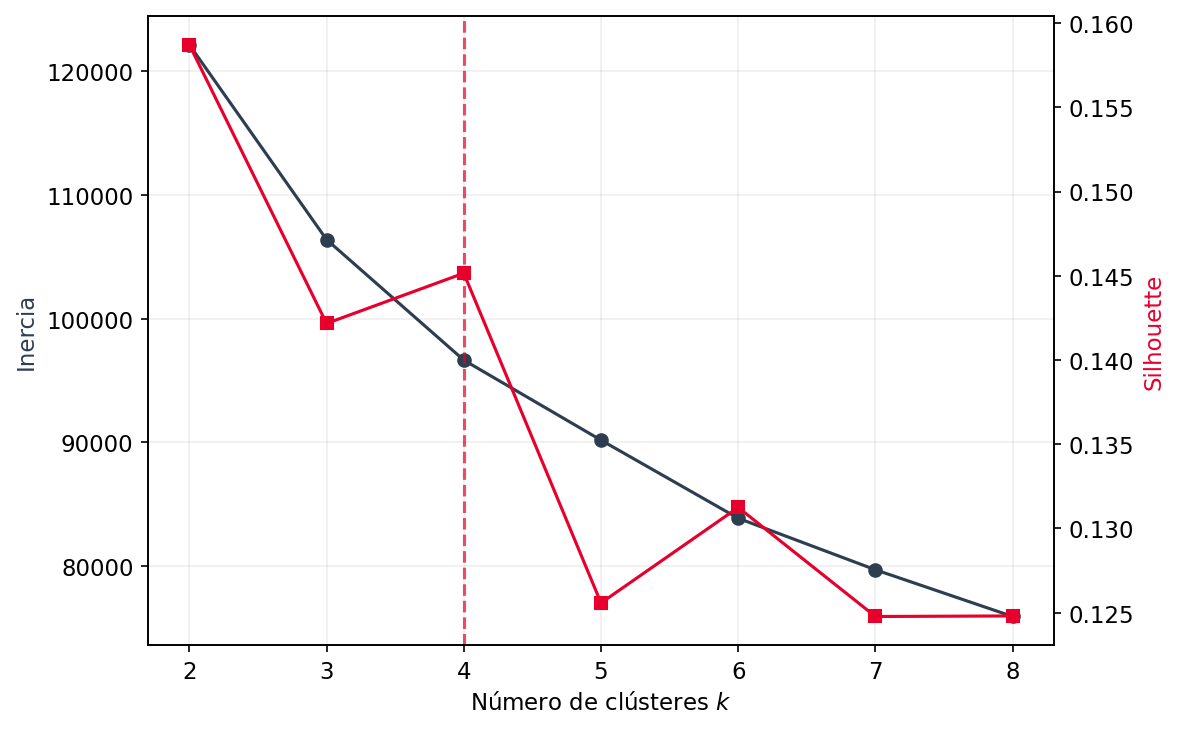
\includegraphics[width=0.85\textwidth]{elbow_laps.png}
  \caption{Selección de $k$ para el clasificador de tipo de vuelta: inercia (codo) y coeficiente de Silhouette frente al número de clústeres. El máximo del Silhouette se alcanza en $k=4$.}
  \label{fig:elbow}
\end{figure}
 
\noindent Este análisis se recoge en las figuras \ref{fig:elbow_pilotaje} y \ref{fig:elbow_circuitos} para los clasificadores de pilotaje y de circuito, respectivamente.

\begin{figure}[H]
  \centering
  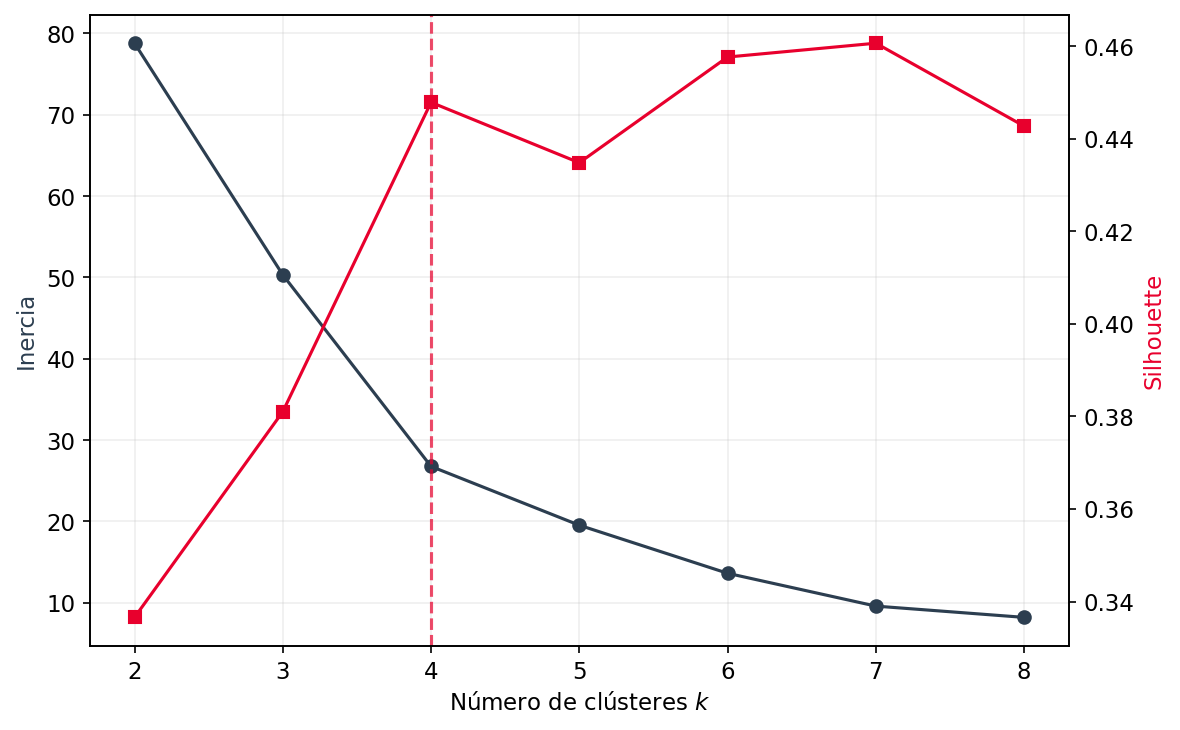
\includegraphics[width=0.85\textwidth]{elbow_pilotaje.png}
  \caption{Selección de $k$ para el clasificador de estilo de pilotaje. En $k=4$ el silhouette es de 0,45, a solo 0,01 del máximo, pero con grupos interpretables y sin fragmentar en exceso a los pilotos.}
  \label{fig:elbow_pilotaje}
\end{figure}

\begin{figure}[H]
  \centering
  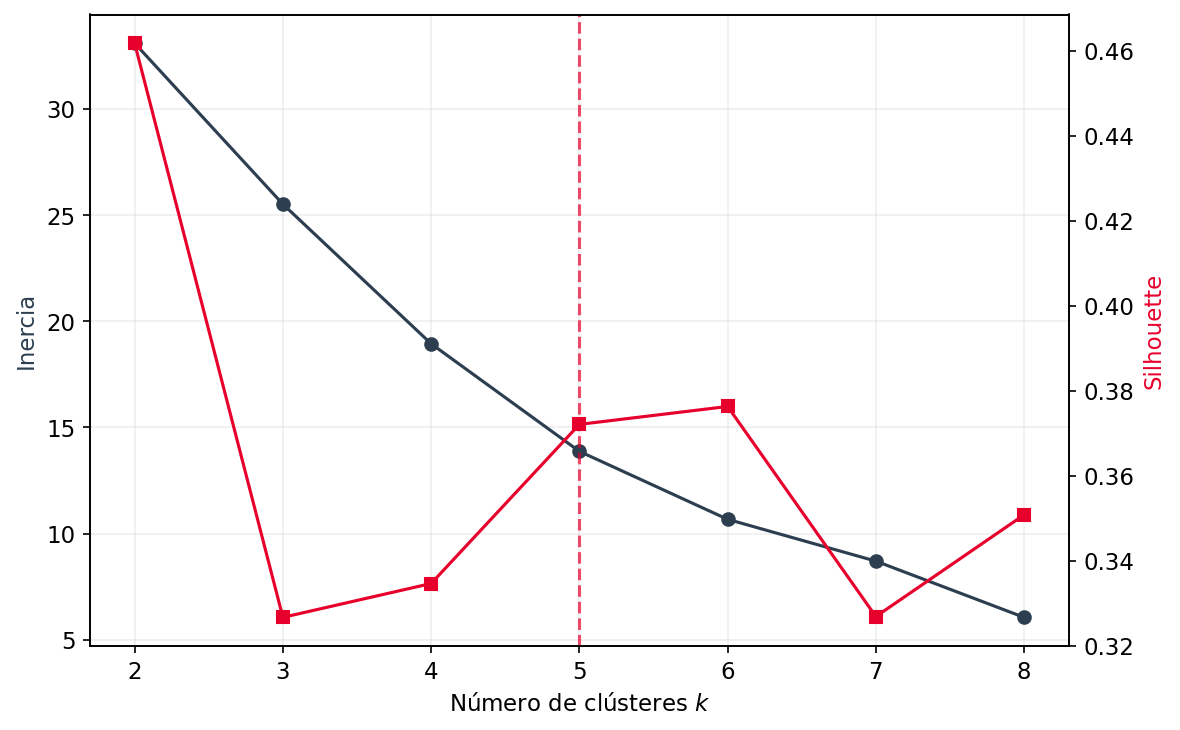
\includegraphics[width=0.85\textwidth]{elbow_circuitos.png}
  \caption{Selección de $k$ para el clasificador de circuitos. Se adopta $k=5$ por la interpretabilidad de las cinco tipologías resultantes, pese a que un $k$ menor ofrezca un silhouette superior.}
  \label{fig:elbow_circuitos}
\end{figure}

\subsection{Resultados}
La tabla \ref{tab:metricas_clasificadores} recoge las métricas de los tres clasificadores sobre el modelo desplegado, y las figuras \ref{fig:cluster_circuitos} y \ref{fig:cluster_pilotaje} muestran la separación de los clústeres proyectada sobre las dos primeras componentes principales.

\begin{table}[htbp]
\centering
\small
\begin{tabular}{@{}lccccc@{}}
\toprule
\textbf{Clasificador} & \textbf{$k$} & \textbf{Silhouette} & \textbf{Davies-Bouldin} & \textbf{Calinski-H.} & \textbf{ARI} \\
\midrule
Pilotaje        & 4 & 0,45 & 0,65 & 26,8   & 1,00 (LOO) \\
Circuito        & 5 & 0,37 & 0,67 & 22,0   & 0,93 (LOO) \\
Tipo de vuelta  & 4 & 0,15 & 1,73 & 3007,8 & 0,98 (5-fold) \\
\bottomrule
\end{tabular}
\caption{Métricas de validación de los tres clasificadores. ARI obtenido por validación cruzada (\textit{leave-one-out} para circuito y pilotaje, dado su menor tamaño, y 5-\textit{fold} para tipo de vuelta).}
\label{tab:metricas_clasificadores}
\end{table}

\noindent Los resultados han de leerse con honestidad. Los clasificadores de pilotaje y de circuito presentan coeficientes de silhouette razonables e índices de Davies-Bouldin bajos, lo que indica que los grupos están bien definidos.
El clasificador de tipo de vuelta presenta un Silhouette bajo, lo cual refleja la naturaleza continua de los datos.

\noindent Cabe aclarar que el índice de Calinski-Harabász depende del tamaño de la muestra, por lo que solo es comparable entre valores de $k$ de un mismo clasificador, no entre distintos.

\noindent La proyección de los clústeres sobre sus dos primeras componentes principales confirma visualmente esta lectura. En los circuitos de la figura \ref{fig:cluster_circuitos} los grupos aparecen claramente separados y Mónaco queda completamente aislado, coherente con su carácter de trazado Urbano Extremo.

\begin{figure}[H]
  \centering
  \begin{minipage}{0.49\textwidth}
    \centering
    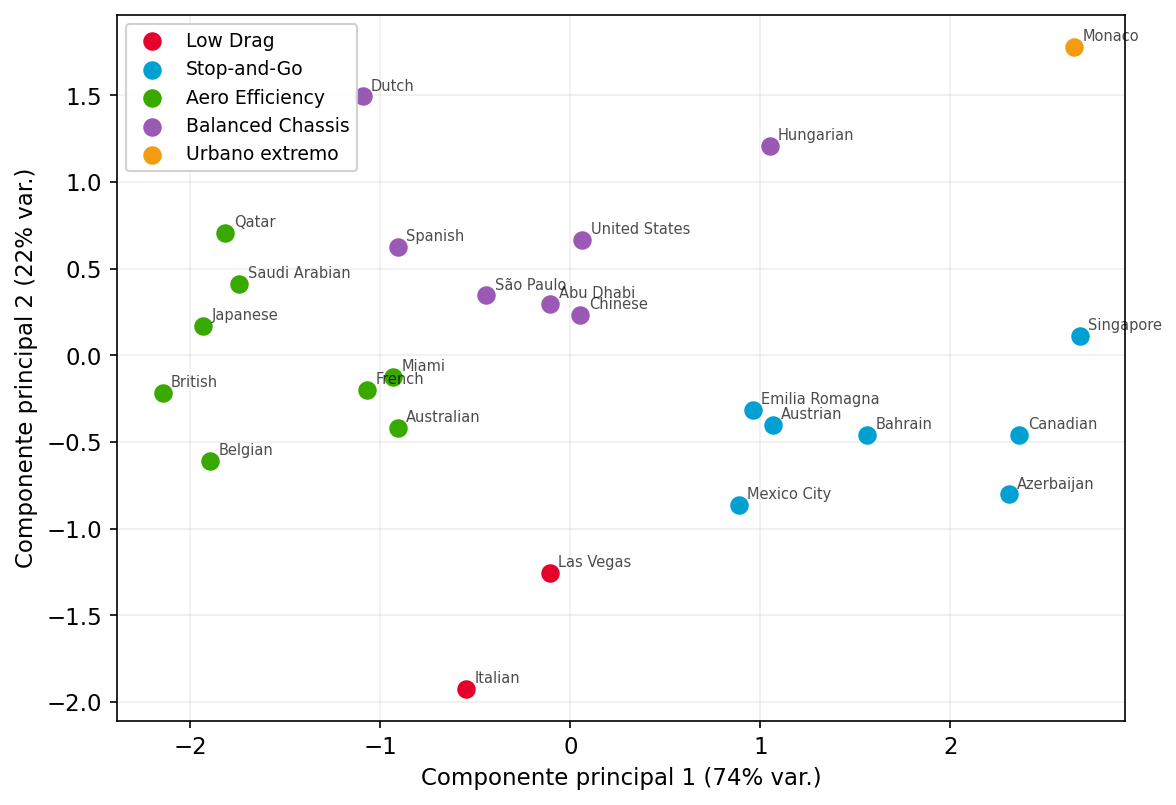
\includegraphics[width=\linewidth]{cluster_circuitos.png}
    \caption{Clústeres de circuitos proyectados sobre sus dos componentes principales (95,8\% de la varianza). Mónaco queda completamente aislado del resto, confirmando su carácter de trazado único.}
    \label{fig:cluster_circuitos}
  \end{minipage}\hfill
  \begin{minipage}{0.49\textwidth}
    \centering
    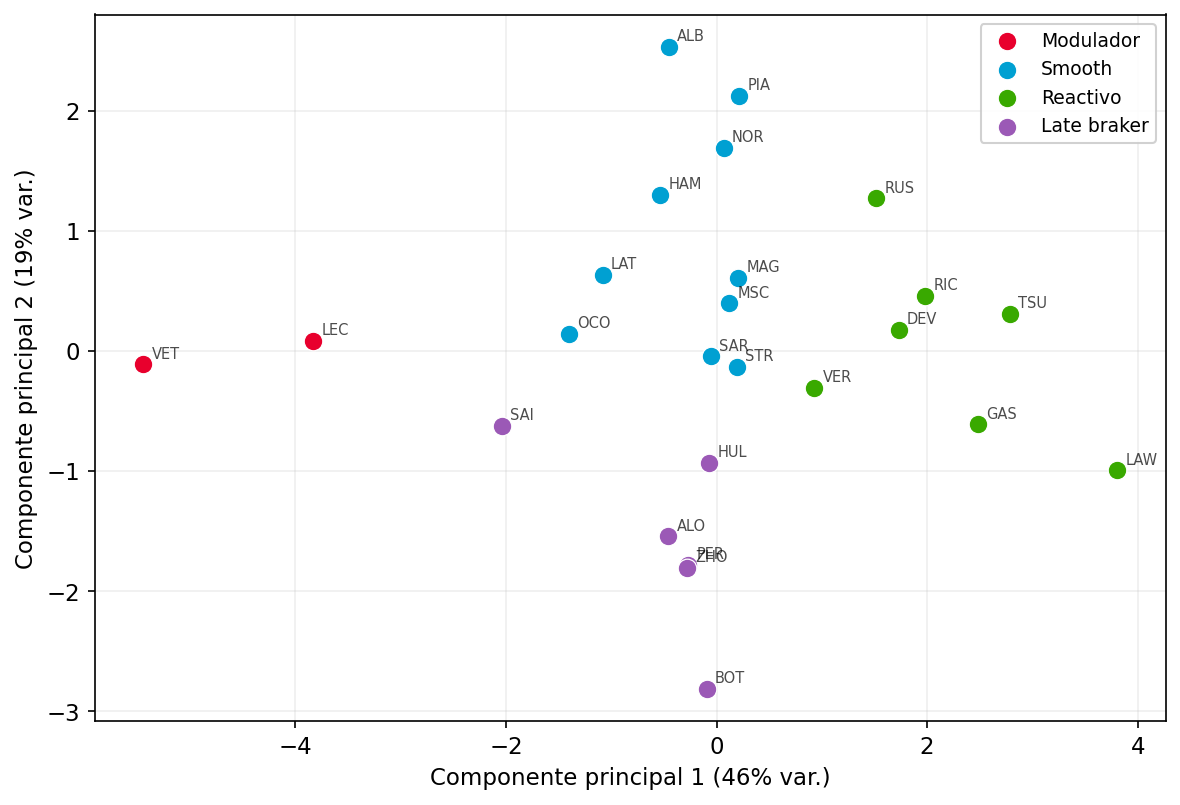
\includegraphics[width=\linewidth]{cluster_pilotaje.png}
    \caption{Clústeres de estilo de pilotaje proyectados sobre sus dos componentes principales (64,5\% de la varianza), que sustentan la separación de los cuatro perfiles.}
    \label{fig:cluster_pilotaje}
  \end{minipage}
\end{figure}

\noindent Los estilos de pilotaje de la figura \ref{fig:cluster_pilotaje} también se distinguen sobre sus componentes principales, sustentando la separación de los cuatro perfiles.
En esto se puede ver cómo pilotos de la escudería Ferrari tienen un mismo estilo (posible sesgo de coche).

\noindent Como limitación principal, la estabilidad temporal del clasificador de pilotaje es baja entre temporadas distintas. Esto es esperable, ya que la firma de un piloto evoluciona con los cambios de coche y reglamento de cada año.
\noindent No obstante, lo determinante es que, pese al solapamiento, las particiones son muy estables: el ARI alcanza valores de 0,93, lo que confirma que las asignaciones son reproducibles.

\chapter{Conclusiones y Trabajos futuros}
Este trabajo partió de una convicción simple: los datos de Fórmula 1 ya son públicos y accesibles, y lo que faltaba era una forma gratuita de explorarlos a fondo. Este proyecto materializa esa visión en una herramienta de análisis que cubre, en un único sistema integrado, gran parte del dominio.

\noindent A lo largo del desarrollo se han construido catorce módulos de análisis agrupados en cuatro categorías funcionales, tres clasificadores de aprendizaje no supervisado y un módulo de dinámica vehicular que deriva magnitudes de la telemetría. La arquitectura resultante es modular, reproducible e instalable en cualquier sistema Windows y Linux con Python sin dependencias de pago.

\noindent Desde el punto de vista técnico los principales retos abordados han sido el procesamiento de telemetría y muestreo irregular, las magnitudes físicas y el diseño de clasificadores no supervisados que ofrecen etiquetas interpretables, así como montar la aplicación funcional desde cero.
La validación cuantitativa de los clasificadores afirma que, aunque hay una separación moderada por la naturaleza del dominio, la estabilidad es alta.

\noindent El desarrollo dejó también varias lecciones. La principal fue trabajar con datos reales que obligan a diseñar en torno a su imperfección, la telemetría llega con un muestreo irregular, dañada o con datos de ruido que obligó a procesarlas para poder compararlas. Las fuerzas G y las posiciones GPS exigieron un filtrado de ruido y en general, cada decisión técnica vino impuesta por una limitación concreta de los datos, no por una preferencia previa.

\noindent Otra lección surgió de los clasificadores. Fue el primer contacto con el aprendizaje no supervisado a un dominio real, y el principal reto no fue técnico sino conceptual al agrupar un fenómeno continuo que carece de fronteras nítidas. Elegir el número de grupos  equilibrando las métricas con el significado del dominio, y dar a cada clúster una etiqueta con sentido, enseñó que en este tipo de problemas la interpretabilidad pesa tanto como cualquier indicador numérico.

\noindent En cuanto al público objetivo, TALOS ha sido diseñado para ser útil en un espectro amplio de usuarios, desde el aficionado ocasional que quiere entender por qué su piloto favorito perdió la carrera hasta el entusiasta técnico que compara fuerzas G en trazados distintos. La ausencia de barreras de entrada (gratuito, sin registro, sin conocimientos de programación)
es en sí misma parte del objetivo del proyecto.

\section{Trabajo Futuro}
El alcance de este trabajo deja abiertas varias líneas de mejora que se identificaron durante el desarrollo y la validación, y que representan extensiones naturales del sistema.

\noindent \textbf{Clasificador de tipo de vuelta con pertenencia suave}: El bajo Silhouette del clasificador refleja la naturaleza continua del estilo de conducción, una mejora conceptual sería sustituir k-means por un modelo distinto para modelar de una mejor manera el clasificador sin depender de fronteras discretas. 

\noindent \textbf{Integración de telemetría de simuladores}: La arquitectura modular permite añadir nuevas fuentes de datos sin alterar el núcleo de la aplicación. Una extensión natural sería capturar los paquetes UDP que emiten videojuegos como \textit{EA Sports F1} o simuladores como \textit{Assetto Corsa Competizione}, permitiendo a los jugadores comparar su propia telemetría con la de pilotos reales.

\noindent \textbf{Integración de competiciones}: Aunque el deporte objetivo es la Fórmula 1, la herramienta funciona mediante datos que pueden provenir de cualquier fuente. Esto da pie a que, siempre que haya datos disponibles, pueda analizarse cualquier deporte de motor incluyendo competiciones de resistencia como el \textit{World Endurance Championship} o categorías inferiores de Fórmula.

\noindent \textbf{Independencia del proveedor de datos}: Actualmente la aplicación depende directamente de FastF1 como fuente de telemetría. Una mejora estructural sería introducir una capa de abstracción entre la fuente de datos y la lógica de negocio, de modo que un cambio en la API de FastF1, o su eventual discontinuación, no afectara al resto del sistema y permitiera incorporar nuevas fuentes con un impacto mínimo.

%────────────────────── Apéndices ─────────────────────────────────────
\begin{umaappendices}

\umaappendix{Manual de Instalación}\label{app:instalacion}
El código fuente de TALOS está disponible públicamente en el repositorio:
\begin{center}
\url{https://github.com/hgdario/f1-telemetry-dss}
\end{center}

\section{Requisitos previos}
\begin{itemize}
  \item \textbf{Python 3.10 o superior.} Disponible en \url{https://www.python.org/downloads/}.
  \item \textbf{Conexión a Internet.} Necesaria durante la instalación para descargar las dependencias y, en la primera consulta de cada sesión, para que FastF1 descargue los datos desde los servidores de Fórmula 1. Las sesiones consultadas quedan almacenadas en caché local y no requieren conexión en accesos posteriores.
  \item \textbf{Git} (opcional). Necesario para clonar el repositorio; alternativamente puede descargarse el archivo ZIP desde la página del repositorio.
\end{itemize}

\section{Obtención del código fuente}
\begin{lstlisting}[style=bash, caption={Clonado del repositorio}, label={lst:clone}]
git clone https://github.com/hgdario/f1-telemetry-dss.git
cd f1-telemetry-dss
\end{lstlisting}

\section{Instalación en Windows}
En Windows la instalación y el arranque están automatizados mediante scripts \texttt{.bat}

\begin{enumerate}
  \item Instalar Python 3.10 o superior desde \url{https://www.python.org/downloads/}, marcando la opción \textit{Add Python to PATH} durante la instalación.
  \item Ejecutar \texttt{install.bat} con doble clic. El script detecta Python, crea un entorno virtual aislado en \texttt{.venv} e instala todas las dependencias listadas en \texttt{requirements.txt}.
  \item Una vez completada la instalación, ejecutar \texttt{start.bat} para arrancar la aplicación.
\end{enumerate}

\section{Instalación en Linux}
En sistemas Unix el proceso equivalente se realiza desde el terminal. En distribuciones basadas en Debian puede ser necesario instalar previamente el módulo \texttt{venv}.
\begin{lstlisting}[style=bash, caption={Instalación en Linux}, label={lst:install_linux}]
# Solo en Debian/Ubuntu/Mint, si el modulo venv no esta disponible
sudo apt install python3-venv

# Crear y activar el entorno virtual
python3 -m venv .venv
source .venv/bin/activate

# Instalar dependencias
pip install -r requirements.txt
\end{lstlisting}

Para arrancar la aplicación:

\begin{lstlisting}[style=bash, caption={Arranque en Linux}, label={lst:start_linux}]
source .venv/bin/activate
cd src
streamlit run app.py
\end{lstlisting}

\section{Primera ejecución}

Al arrancar, Streamlit abre automáticamente el navegador en \texttt{http://localhost:8501}. La primera vez que se consulta una sesión, FastF1 descarga los datos correspondientes y los almacena en caché local; este proceso puede tardar desde unos segundos hasta varios minutos según la sesión y la conexión. Las consultas posteriores a la misma sesión son prácticamente instantáneas.

\umaappendix{Manual de Usuario}\label{app:usuario}
TALOS se organiza en torno a un flujo de navegación de tres niveles: el usuario parte de un \textbf{buscador de Gran Premio}, selecciona una \textbf{sesión} concreta y accede a un \textbf{hub de módulos} de análisis. Toda la interacción se realiza desde el navegador, sin necesidad de conocimientos de programación.

\section{Buscador de Gran Premio}
La pantalla inicial presenta un mapamundi interactivo con todos los circuitos del calendario del año seleccionado. El usuario puede cambiar de temporada mediante el selector de año situado en la cabecera. Al hacer clic sobre el marcador la aplicación accede a la pantalla de selección de sesión correspondiente. La figura \ref{fig:manual_grid} muestra esta pantalla inicial.
\begin{figure}[ht]
  \centering
  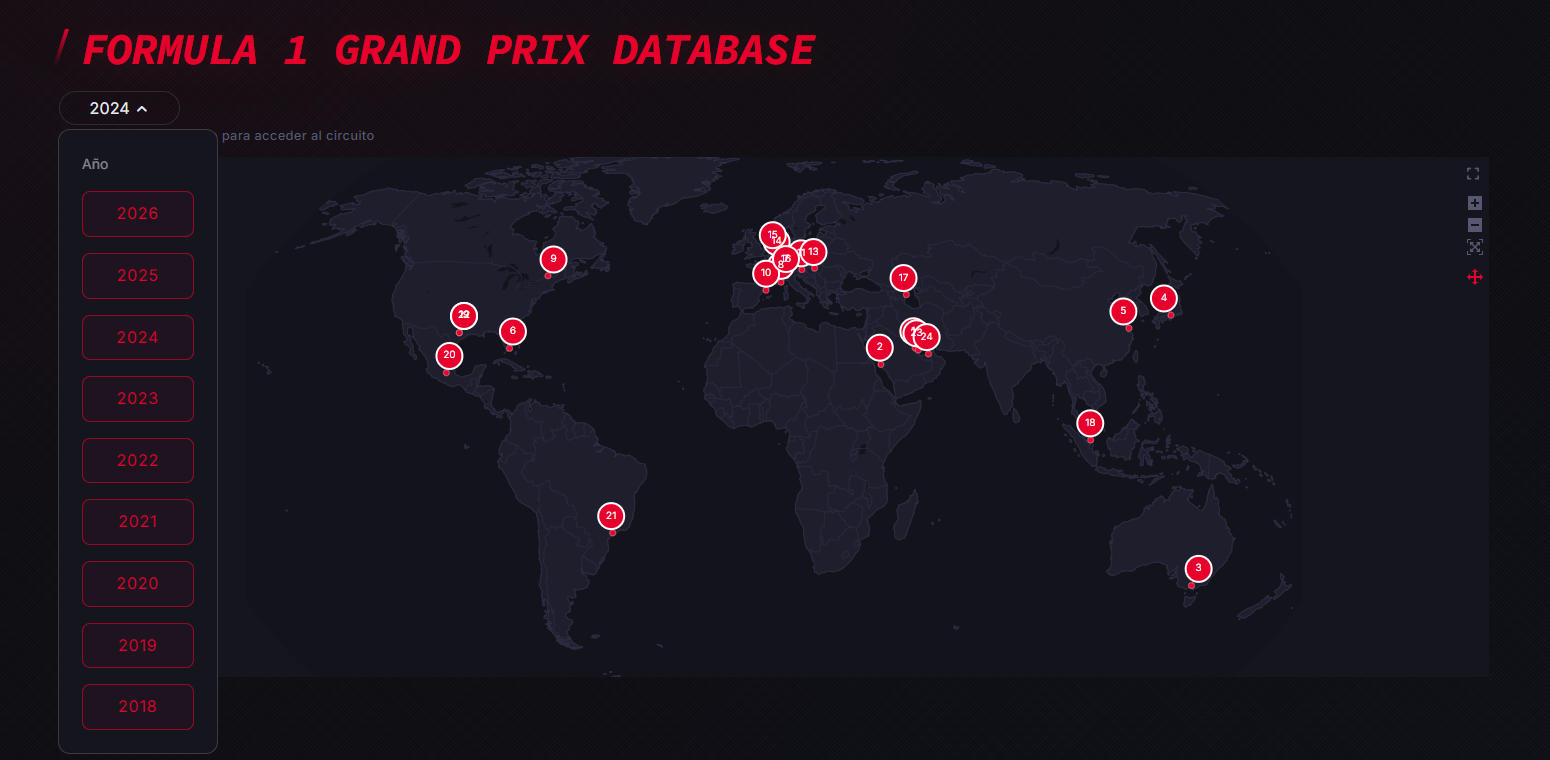
\includegraphics[width=\linewidth]{grid.png}
  \caption{Buscador de Gran Premio: mapamundi interactivo del calendario.}
  \label{fig:manual_grid}
\end{figure}

\section{Selección de sesión}
Una vez seleccionado el Gran Premio, se muestran las sesiones disponibles y las sesiones de formato \textit{Sprint} cuando proceda. Cada sesión se representa mediante una tarjeta, fecha y hora. Al pulsar \textit{Cargar}, FastF1 descarga y sincroniza los datos de dicha sesión, como se muestra en la figura \ref{fig:manual_session}.

\begin{figure}[ht]
  \centering
  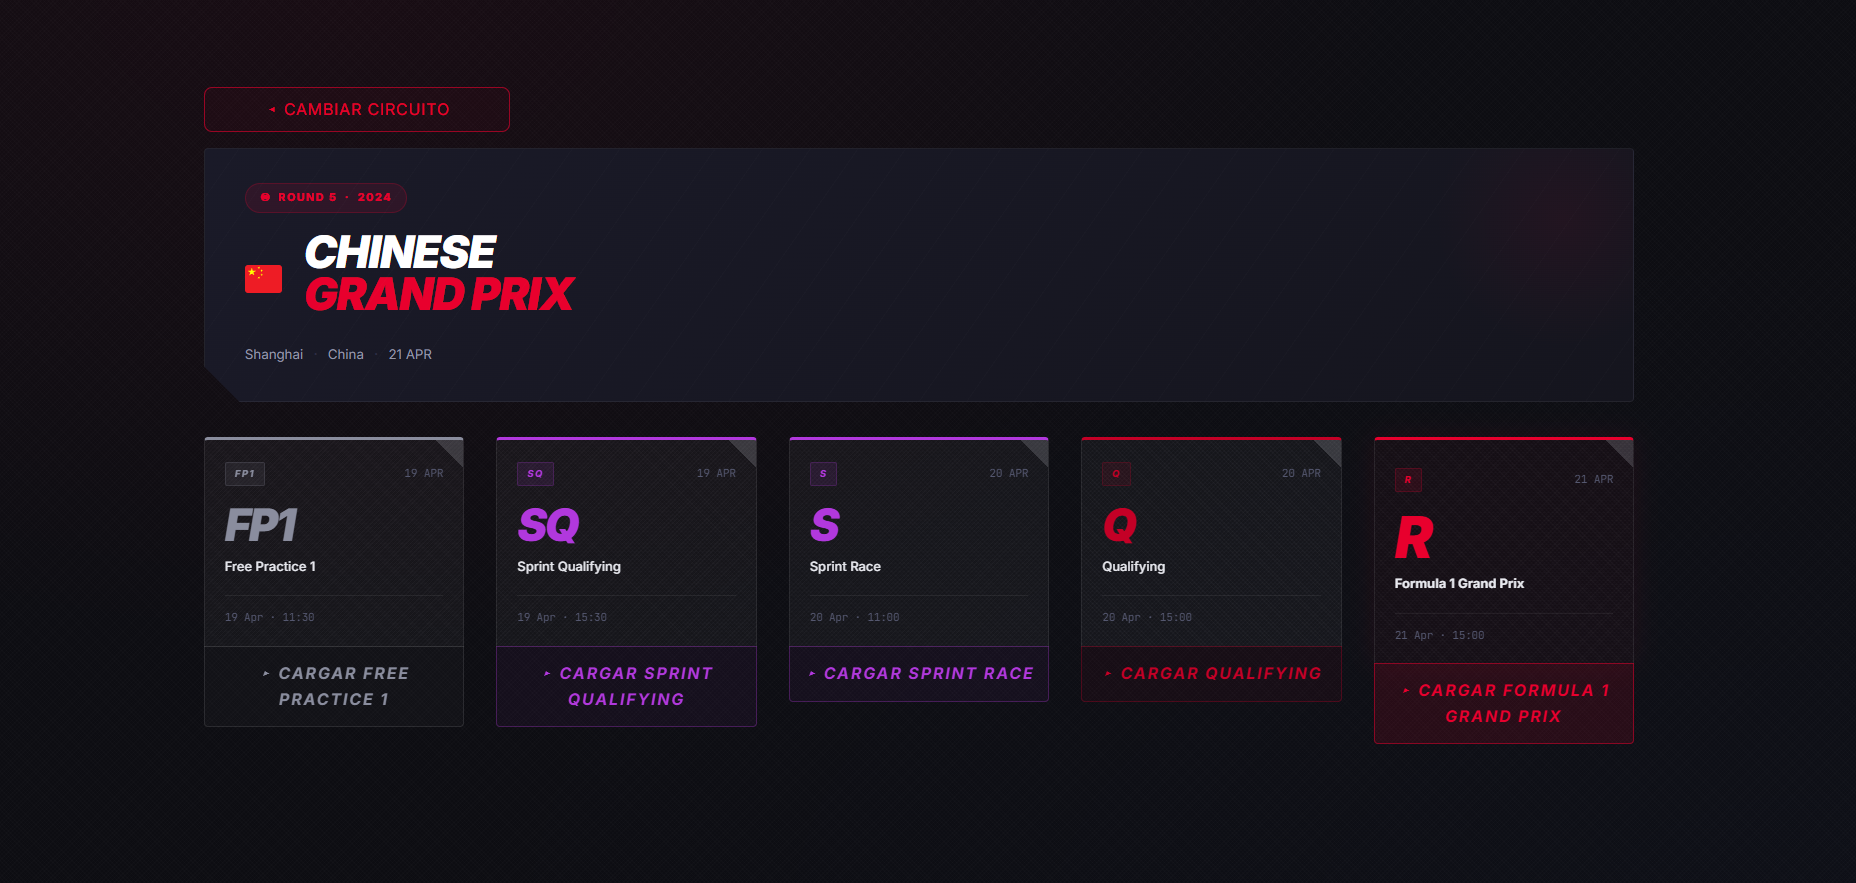
\includegraphics[width=\linewidth]{session.png}
  \caption{Pantalla de selección de sesión del fin de semana.}
  \label{fig:manual_session}
\end{figure}

\section{Hub de módulos}
El hub es el punto central de la aplicación, muestra la sesión activa, un podio con los primeros clasificados y un panel lateral con métricas rápidas y la clasificación final.
Los módulos de análisis se agrupan en cuatro categorías accesibles mediante pestañas. Desde cualquier módulo, el usuario puede volver al Hub. La figura \ref{fig:manual_hub} muestra este panel central.

\begin{figure}[ht]
  \centering
  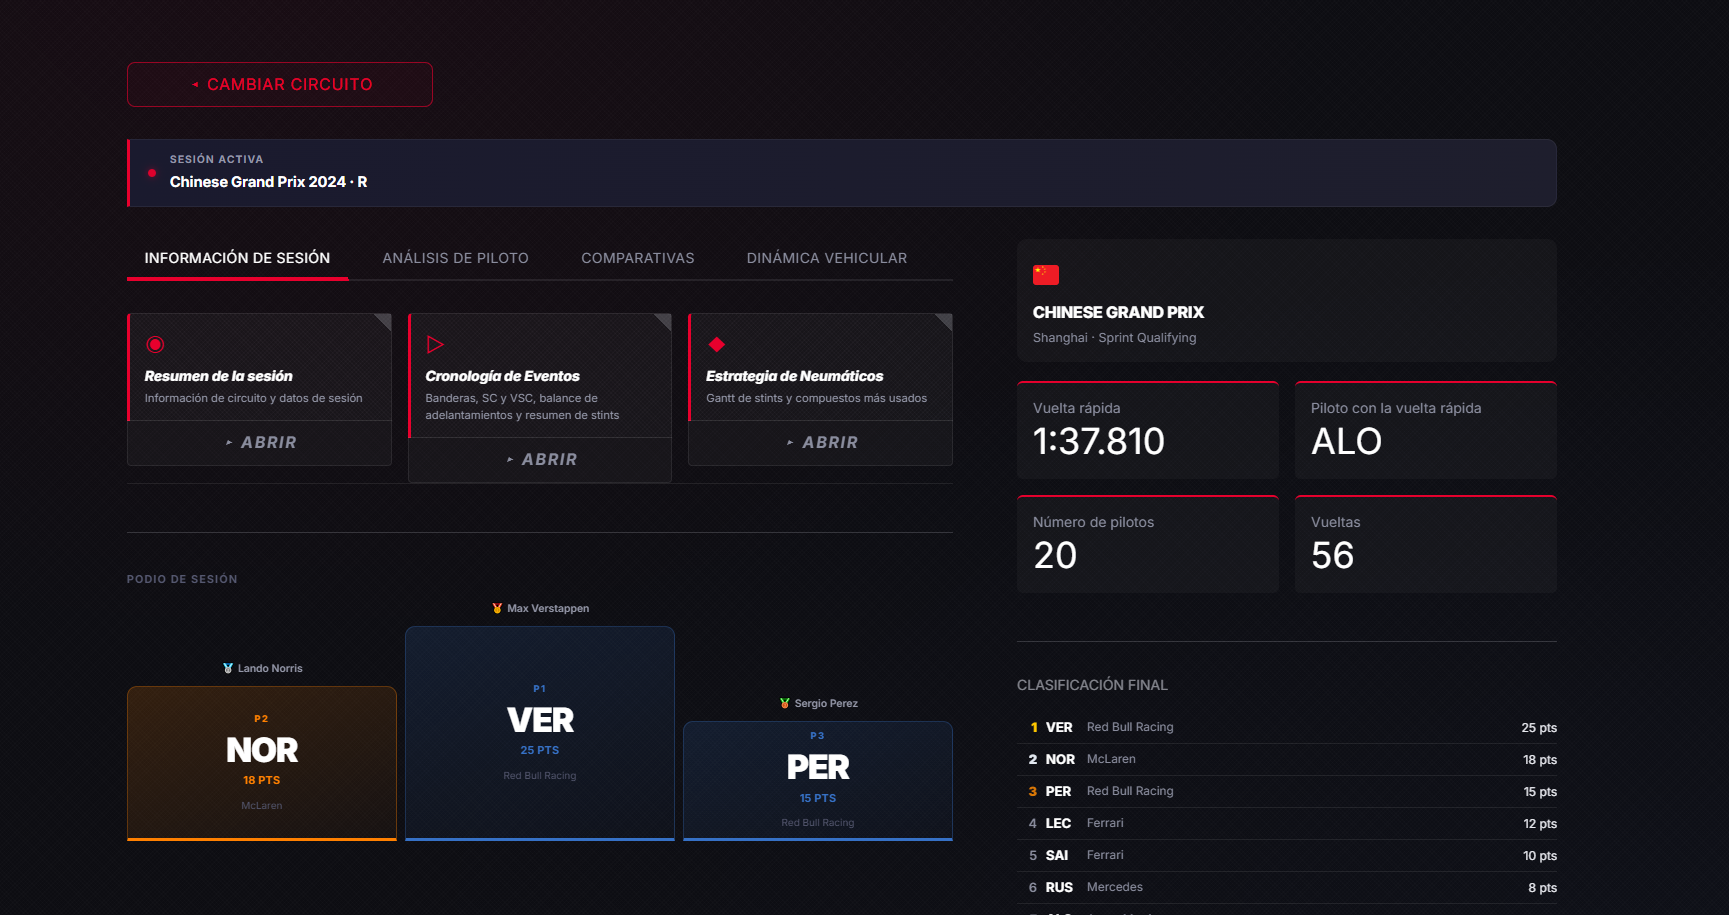
\includegraphics[width=\linewidth]{hub.png}
  \caption{Hub de módulos con la sesión activa, el podio y el panel de métricas.}
  \label{fig:manual_hub}
\end{figure}

\section{Módulos de análisis}
A continuación se describen los catorce módulos disponibles agrupados por categoría.

\subsection{Información de Sesión}
\begin{enumerate}
  \item \textbf{Resumen de la sesión.} Información del circuito y datos generales de la sesión. Se muestran temperaturas relativas al resto de circuitos y datos generales del trazado. Se dibuja el trazado con los sectores coloreados, zonas de velocidad y DRS. Este módulo incluye el clasificador de circuito indicándonos en cuál de las 5 categorías se encuentra.
  \item \textbf{Cronología de Eventos.} Reconstruye el transcurso de la sesión incluyendo las banderas, periodos de \textit{Safety Car} y \textit{Virtual Safety Car}, balance de adelantamientos que compara la posición inicial con la final y un resumen de los \textit{stints} de cada piloto.
  \item \textbf{Estrategia de Neumáticos.}  Muestra, mediante un diagrama de Gantt, los \textit{compuestos} usados por cada piloto y las gomas más utilizadas en toda la carrera, permitiendo comparar las estrategias seguidas a lo largo de la carrera.
\end{enumerate}

\subsection{Análisis de Piloto}
\begin{enumerate}
  \item \textbf{Resumen del Piloto.} Sintetiza la sesión de un piloto concreto indicando claves de rendimiento, tiempos por sector, y KPIs. Sirve como una primera introducción a lo que ha hecho el corredor elegido en la sesión.
  \item \textbf{Mapa de Velocidad.} Trazado del circuito coloreado según la velocidad (km/h) a lo largo de la vuelta seleccionada. Evidencia las zonas de máxima y mínima velocidad.
  \item \textbf{Mapa de Marchas.} Trazado del circuito coloreado según la marcha engranada en cada punto. Esto permite identificar los puntos de cambio y la gestión de caja, así como visualizar en qué marcha toma el piloto cada curva.
  \item \textbf{Telemetry Trace.} Muestra los canales de telemetría del piloto junto con una animación del circuito y una caracterización de su estilo de conducción y tipo de vuelta. Muestra velocidad en todos los tramos del circuito, acelerador y freno, si ha activado o no el DRS, las RPM y marchas.
\end{enumerate}

\subsection{Comparativas}
\begin{enumerate}
  \item \textbf{Panel de Equipo.} Enfrenta a los dos pilotos de un mismo equipo, comparando su telemetría y ritmo para evaluar el rendimiento relativo entre compañeros. Incluye un trazado del circuito donde se puede apreciar el punto exacto del GPS de cada piloto para la vuelta dada. Como se muestra en la figura \ref{fig:manual_panel_equipo}
  \begin{figure}[H]
  \centering
  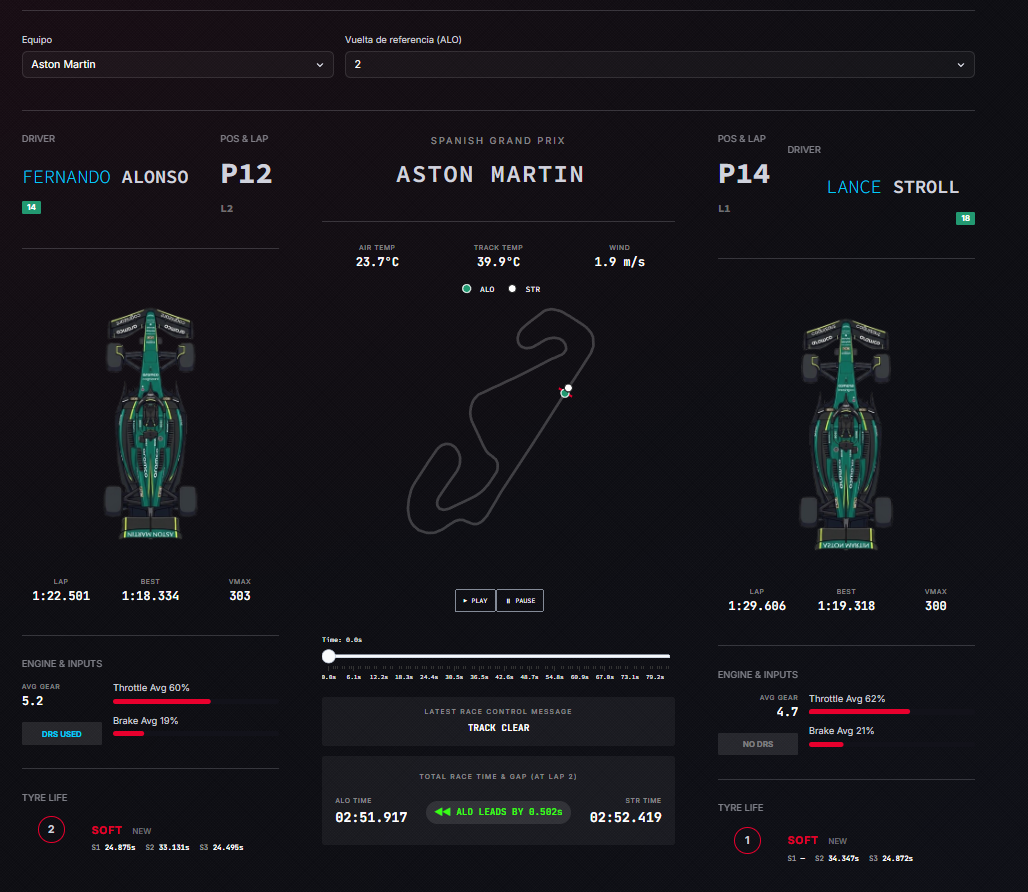
\includegraphics[width=\linewidth]{panelequipo.png}
  \caption{Módulo \textit{Panel de Equipo}: comparación lado a lado de los dos pilotos de una escudería (telemetría, ritmo, neumáticos y circuito animado).}
  \label{fig:manual_panel_equipo}
\end{figure}
  \item \textbf{Comparativa de Sesión.} Superpone (\textit{overlay}) los canales de telemetría de varios pilotos sobre la misma vuelta, facilitando la comparación directa de sus métricas. Incluye una sección de dominancia por circuito en la que se pinta del color del piloto dominante el microsector correspondiente.
  \item \textbf{La Vuelta Ideal.} Reconstruye la vuelta óptima a partir de los mejores microsectores de toda la parrilla, con posibilidad de filtrar por equipos, mostrando el límite teórico de rendimiento.
  \item \textbf{Coche Fantasma.}  Genera una animación 2D de persecución que enfrenta las vueltas de dos pilotos sobre el trazado, visualizando dónde y cuánto gana tiempo cada uno.
\end{enumerate}

\subsection{Dinámica Vehicular}
\begin{enumerate}
 \item \textbf{Diagrama G-G.} Representa el círculo de tracción y la envolvente de fuerzas G (longitudinales y laterales) del monoplaza, mostrando el aprovechamiento del agarre disponible.
  \item \textbf{Carga Aerodinámica.} Ofrece una estimación teórica de la carga aerodinámica a partir de la relación entre la aceleración lateral y la velocidad del coche.
  \item \textbf{Mapa de Carga por Rueda.} Estima la distribución de carga por eje y la temperatura de frenos a lo largo de la vuelta, ilustrando las transferencias de peso en frenadas y curvas.
\end{enumerate}

\section{Selección de piloto y vuelta}
Los módulos centrados en un piloto concreto incorporan dos selectores comunes: uno para elegir el piloto y otro para la vuelta a analizar. Por defecto se selecciona la vuelta más rápida del piloto. Adicionalmente
se incluye la opción de mostrar curvas que superpone la numeración de las curvas sobre las visualizaciones que lo permiten.
\end{umaappendices}
%────────────────────── Back cover and bibliography ────────────────────
\backmatter
\printbibliography[title={Bibliografía}]
\cleardoublepage
\MakeUMABackCover

\end{document}
% ======================================================================
